\documentclass[12pt]{report}

\usepackage[utf8]{inputenc}
\usepackage{graphicx}
\graphicspath{ {images/} }
\usepackage{caption}
\usepackage{subcaption}
\usepackage{float}
\usepackage[a4paper,width=150mm,top=35mm,bottom=25mm,bindingoffset=0mm]{geometry}
\usepackage{fancyhdr}
\usepackage{setspace}
\usepackage{amsmath}
\usepackage{tabularx}
\usepackage{makecell}
\usepackage{lscape}
\usepackage{hyperref}
\usepackage{CJKutf8}
\usepackage{booktabs}
\usepackage{longtable}
\usepackage{upgreek}
\usepackage{array}
\pagestyle{fancyplain}% <- use fancyplain instead fancy
\fancyhf{}
\fancyhead[R]{\thepage}
\renewcommand{\headrulewidth}{0pt}
\setlength{\headheight}{12pt}

\usepackage{titlesec}
\captionsetup[table]{position=top} % Set table captions on top
\captionsetup{font=small} % Bold labels and set font size to small

% --- ADD THESE LINES ---
\usepackage{helvet} 
\captionsetup[subfigure]{labelfont={sf}} 
% -----------------------

\titleformat{\section}
  {\normalfont\fontsize{18}{15}\bfseries}{\thesection}{1em}{}

  
\usepackage[backend = biber, style=ieee,sorting=none]{biblatex}
\addbibresource{references.bib}	

\title{Thesis Title}
\author{Author Name}
\date{Day Month Year}

\begin{document}
\pagenumbering{roman} 

\begin{titlepage}
	\vfill
    \begin{center}
        \Large
        Nagoya University\\
        Global 30 International Programs

        \begin{center}
                        
\includegraphics[width=\textwidth]{images/figures_titlepage/Logo.png}
                    \end{center}
        \vspace*{1.0cm}

        
        
        \huge
        \textbf{Implementation of Flatwise Windings for Improved Thermal Management in Transformers for Solid State Transformer (SST) Applications}

        \vspace{0.5cm}
        \Large\textbf{
        Solid State Transformer (SST) \begin{CJK}{UTF8}{min}用変圧器 (トランス) の高放熱フラットワイズ巻線構造の提案\end{CJK}}

        
        \vspace{1.0cm}
        \large
        \textbf{August 2026}
        \vspace{1.0cm}
        \normalsize
        
        \textbf{Karl Raymond Dela Cruz Roque}\\
        282448024\\
        G30 Automotive Engineering Program\\
        Electrical Engineering, Electronics, and Information Engineering\\
        \textbf{Yamamoto Laboratory for Power Electronics}\\
        \normalsize
        \vspace{1.5cm}
        A Master's Thesis\\ Submitted to the Department of Electrical Engineering, Electronics, and Information Engineering\\ Nagoya University\\In partial fulfillment of the requirements \\For a Degree in \\
        
        Master of Engineering in Automotive Engineering - Electrical Engineering, Electronics, and Information Engineering 
        
        
        
        
    
        
        \vspace{1.8cm}

        
        
        
        
        
    \end{center}
    \vfill
\end{titlepage}

\setstretch{1.5} 
\fancyhf{} % clear all header and footer fields
\fancyhead[RO,R]{\thepage} %RO=right odd, RE=right even
\renewcommand{\headrulewidth}{0pt}

\begin{center}
    \LARGE
    \textbf{Abstract}
\end{center}
\singlespacing
\par Increased energy generation and consumption are imminent as economies develop and the drive towards electrification intensifies. To keep up with the increasing energy demands of society, the Solid State Transformer (SST) is a critical and rising technology to facilitate energy conversion and distribution, replacing the traditional line frequency transformer to achieve higher power density and advanced functions, made possible by the advent of fast-switching wide band-gap (WBG) semiconductor devices. However, effective thermal management for the transformer in the isolation stage of the SST is one of the primary design bottlenecks for high-power transformers as current methods can compromise the power density of the converter. 
\par This study investigates a contrasting design approach that prioritizes intrinsic thermal performance of the transformer utilizing rectangular windings, which has the potential to reduce reliance on conventional cooling systems. While rectangular windings offer high fill factors and current capabilities, research comparing the thermal characteristics of different winding orientations remains limited. This paper proposes a low-profile transformer utilizing flatwise windings, characterized by rectangular conductors stacked radially from their broad face. This configuration creates a fundamentally lower thermal resistance path by enabling direct, simultaneous, and parallel heat extraction from every turn as compared to its conventional, edgewise counterpart. A thermomagnetic FEM analysis under the same magnetizing inductance, window area, wire geometry, and current density comparing the proposed design against an edgewise structure at 1 kW demonstrates a peak temperature reduction of 10.9°C (56.0°C vs. 66.9°C) under natural cooling and 13.4°C (30.2°C vs. 43.6°C) under forced air cooling. The results also confirm that the proposed flatwise-wound transformer ensures a uniform heat distribution. Moreover, the consistency of the performance was evaluated spatially through the variation of conductor thickness.
\par A representative edgewise-wound and flatwise-wound transformer with a square window area was implemented in a 100 V:100 V, 1-kW CLLC bidirectional resonant converter at 28.5 kHz switching frequency for experimental comparison under natural and forced-air cooling conditions. The experimental results in both cooling conditions validated the thermal superiority of the flatwise structure, demonstrating lower peak winding temperatures and reduced thermal gradients between the winding and the outer surfaces of the transformer. These results validate the superior thermal performance of the flatwise structure, paving the way for more compact, power-dense transformers. Furthermore, a comprehensive design methodology and trade-off analysis for the proposed transformer are presented.
\par \textbf{Keywords}: Solid State Transformer (SST), Flatwise Windings, Edgewise Windings, Transformer Thermal Management, Transformer Design, FEA
 
\doublespacing

\tableofcontents


\listoffigures


\listoftables

\doublespacing

\chapter*{Acknowledgements}
\footnotesize
\singlespacing
\par I am thrilled to write yet another acknowledgements page for my second thesis during my three-and-a-half-year stay at the Yamamoto Laboratory for Power Electronics. I truly wouldn't have made it without all of you. Thank you to everyone in the laboratory for your support and help, and for being there through both the most challenging times and the happiest of times. \begin{CJK}{UTF8}{min}3年間半、大変お世話になりました。\end{CJK} And after all of this, I could say that I am more confident and even excited for the next step of my journey. Thank you for helping me grow both profesionally and personally throughout my stay here.

\par \begin{CJK}{UTF8}{min}樹へ、プロジェクトの最初から最後まで、心から誠にありがとうございます！まだ言ってなかったけど、最初は樹のこと本当に怖い人かなって思ってました（笑）。でも、全然そんなことなかったです。私の質問はたまに（というかいつも？笑）本当にバカだったと思うけど、\end{CJK}thank you for being very patient with a guy like me. Thank you for helping me see the light in what I do, especially when things seemed to be hopeless. \begin{CJK}{UTF8}{min}樹と共同研究できたことは、私の人生においてかけがえのない経験になりました。またDrinking Partyしようね！\end{CJK} Wishing you all the best, and hopefully we can collaborate again next time. 

\par To Thiyu, thank you so much for always teaching me the fundamentals and helping me get started in the lab, guiding me to where I am today in my research. You were the inspiration behind why I wanted to be part of the group, in case you didn't know. To summarize it all, I wouldn't have formed my own research identity and made it here up to where I am now without you. Thank you for always checking on me, cheering me up, and helping me in every way possible, even if we work with completely different things. And I really like how we try out new and different ideas in the laboratory! A conference is never fun without you, and thank you for always supporting me in my ideas and the things I want to do. I wish you all the best in the last year of the grind and make sure to rest and have fun.
\par To Jiyoon, thank you for being a really good senpai to me. Thank you for also helping me figure out a lot of things as well when I was getting started at the lab, and also for helping me figure out a lot of stuff related to my research as well in my Master's degree. I really appreciate every time you check on me and giving me advice in my future career options! You remain an inspiration to me on how to balance research and life, and I aspire to be like you next time. I wish you all the best in your future endeavors!

\par To Kouta-chan and Shunki Hashimoto, who are now doing their best in the field, thank you as well for all the help and good times in the laboratory. I miss you guys so much. I think I might have been a bit too serious this past year, yet I appreciate you always taking the time to talk with me and helping me with even the simplest and stupidest of things. Thank you as well for keeping me sane and assisting me with various parts of my Master's research. I hope our paths cross again sometime in the future.  

\par To Sihoon (\textit{who is now a Sensei!}), thank you for welcoming me back into the lab when I was still an intern four years ago. You've been a really good \textit{senpai} to me, and now look, you've grown to be a \textit{sensei}. I know I may not have always met your expectations, but thank you for your patience, for constantly pushing me, and for supporting me every step of the way—from helping me prepare papers for my dream conferences, to pushing me to go the extra mile, all the way to our recent journal submission and revision. You've taken me into the Control Team back then, but you helped me find my true passion in this very wide field. And most importantly, thank you for inspiring me to pursue an exciting next chapter that I never expected at all. You helped me understand what it means to do research and the standard it takes to be a good researcher. And indeed, \textit{Pain = Gain}. Thank you for all the advice that got me to where I am today. (And, I'm sorry for not playing futsal always haha!)

\par To my \textit{kouhais}, Kang Mingsung, Gaku Kondo, Yoshida, Miyata, Yuga, and Nozaki-kun, and everyone else, thank you for all the fun moments, your hard work in the lab, and for always keeping the atmosphere so lively. And most especially, thank you for your support and always cheering me on especially when I was at my busiest and perhaps lowest part of my research. I wish you all the best in your own research journeys! 
\par To Raymond, thank you for being a really good junior to me and supoporting me during my time in the laboratory. I was really surprised but very happy that you went into our laboratory. I really had a good privilege working with you and supervising you as well at some point during our stay here, and I was really grateful for that, and we even got to write a paper! Just so you know it was one of my other inspirations as well to continue further studies, as it was a good experience and I want to keep mentoring my juniors as well. I learned so much from you, and I apologize for being too hard on you sometimes. But I hope you learned from me as well! All the best as well for your future endeavors, and keep up the good work that you have now.

\par To the Passive Components Team, thank you for welcoming me into your team. I started with zero knowledge. But everyone of you kept inspiring me to keep learning and trying. Up to when I became a Team Leader during my last six months. Thank you for giving me the opportunity to do so, and I really enjoyed my time with everyone. Hopefully, we can work again together in the future. Oh, and especially, the nomikais. Really gonna miss them especially with you guys.

\par And of course, I want to take the chance to thank Imaoka Sensei for agreeing to be my adviser. I developed an interest in passive components after finishing my bachelor's thesis, yet I knew I was a humble beginner. Thank you for taking me in and being very patient with me, as when I started two years ago, I really did not know a lot about passive components, but when I heard that we will be working with ambitious partners abroad, I just said yes and I wanted to really take the challenge. And I knew it was going to be okay, because you were there. We went through all the challenges together with Itsuki—brainstorming for a topic and finally getting to work in a unique but challenging collaborative research setup with our partners from Finland. Most especially, thank you for the never-ending support of all my dreams, especially concerning my future. You went the extra mile and opened up a lot of opportunities for me, which I am forever grateful for. I promise you that I will contribute to my country in the future, just as you'd always tell me.  

\par To our secretaries, thank you so much for always assisting me with the endless paperwork (which I always do have), answering my many questions, and making the administrative side of lab life so much easier. Thank you as well for always checking on me and ensuring my well-being.

\par Lastly, I would also like to take the chance to thank Yamamoto Sensei for accepting me into this laboratory back in my third year of undergraduate studies. All of this would not have been possible if it were not for that. Ever since, his never-ending support has always kept me on the ground. Thank you for always checking on me and giving me advice, especially regarding the next steps in my career. I will always take care of my health, as you always remind me to do so, and hopefully will do better in my love life as well \begin{CJK}{UTF8}{min}笑\end{CJK}

\par I would also like to thank my friends here in Japan, to those who left, and to those at home, my \textit{kouhais} and \textit{senpais}, who have cheered me on from the very beginning. Oh, and I must not forget, my NUFSA Family!

\par I dedicate this work to my family—Mama, Papa, Kuya, Boy, Ate Ruby, and Achie—who have always been there to listen to all my struggles even if they do not understand a single thing about my work, which became even more complex during my Master's degree. \textit{I did it again!} You have helped keep me going until today, and this is for you.

\par This is also for the Filipino People. I'm almost there. I promise that this is all for the betterment of our home. I can't wait to go back in the future! \textit{Para sa Bayan! Para sa inyo ang lahat ng ito.}
\par And of course, this is also for God, for helping and guiding me all throughout my studies and helping me reach where I am today.

\normalsize
\doublespacing

\chapter{Introduction}
\pagenumbering{arabic} 

According to the U.S. Energy Information Administration (EIA), global energy consumption is projected to increase by 50\% by 2050, relative to 2019, as shown in Figure \ref{fig:energyconsumption}\cite{eia_ieo2019}. This massive surge is largely driven by strong economic and population growth in non-OECD\footnote{Organisation for Economic Co-operation and Development} countries, particularly in Asia, alongside rapid urbanization and rising regional incomes. Accompanied with the ongoing shift toward electrification in end-use sectors, electricity generation is projected to increase by 79\% between 2018 and 2050, as explained in Figure \ref{fig:electricitygeneration}. Meeting this surging energy demand while simultaneously mitigating climate impact has made the transition to carbon neutrality an essential global imperative. This paradigm shift requires unprecedented cooperation across all sectors and has significantly accelerated the deployment of distributed renewable energy resources, which are projected to be the fastest-growing global energy source, alongside electrified transportation, as seen in Figure \ref{fig:renewablenergy}.
\begin{figure}
    \centering
    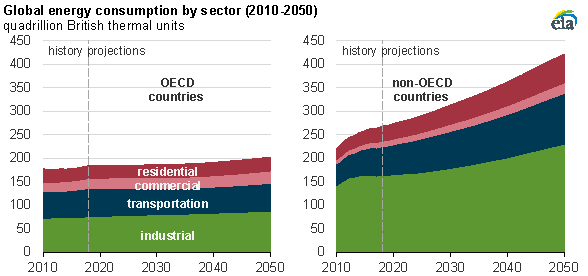
\includegraphics[width=0.9\columnwidth]{figures_intro/projection_energyuse.pdf}
    \caption{Projected increase in global energy consumption by 2050: (left) in OECD Countries, (right) in developing countries.}
    \label{fig:energyconsumption}
\end{figure}

\begin{figure}
    \centering
    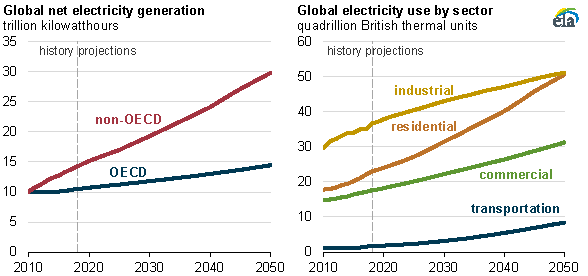
\includegraphics[width=0.9\columnwidth]{figures_intro/intro_energyuse.pdf}
    \caption{Projected increase by 2050 in electricity generation (left) and in electricity use (right) according to different sectors.}
    \label{fig:electricitygeneration}
    
\end{figure}

\begin{figure}
    \centering
    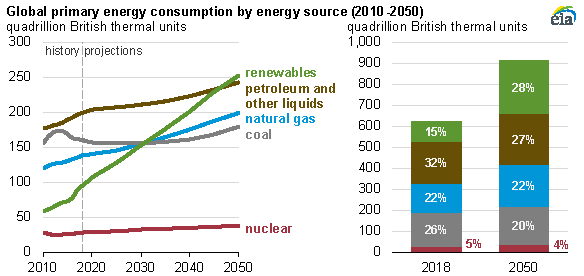
\includegraphics[width=0.9\columnwidth]{figures_intro/renewable_energy.pdf}
    \caption{Projected energy consumption by energy source by 2050.}
    \label{fig:renewablenergy}
\end{figure}
To support this massive, sustainable transition, the underlying electrical distribution infrastructure requires next-generation power conversion systems that are not only highly efficient but also exceptionally compact and reliable. Today, one of the key technologies facilitating these stringent requirements is the Solid State Transformer (SST). SSTs represent an advanced class of power electronic converters equipped with medium-frequency (MF) or high-frequency (HF) galvanic isolation, typically operating between medium-voltage (MV) distribution grids and low-voltage (LV) consumer systems. In this regard, the following sections present the characteristics, applications, and challenges associated with the development of high-power SSTs.

\section{The Solid State Transformer}
The SST is an ongoing trend today in Power Electronics. In higher power applications, to distribute power from the medium-voltage grid to an isolated low-voltage load, the traditional line frequency (50/60 Hz) transformer is commonly used, as represented in Figure \ref{fig:linefrequency}.

\begin{figure}
    \centering
    \subfloat[]{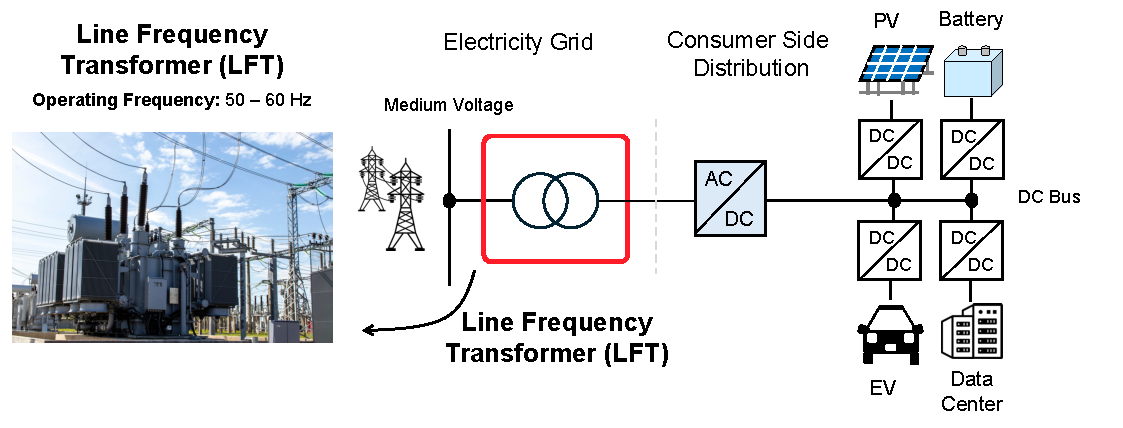
\includegraphics[width=\columnwidth]{figures_intro/linefrequency.pdf}\label{fig:linefrequency}}
\\
    \subfloat[]{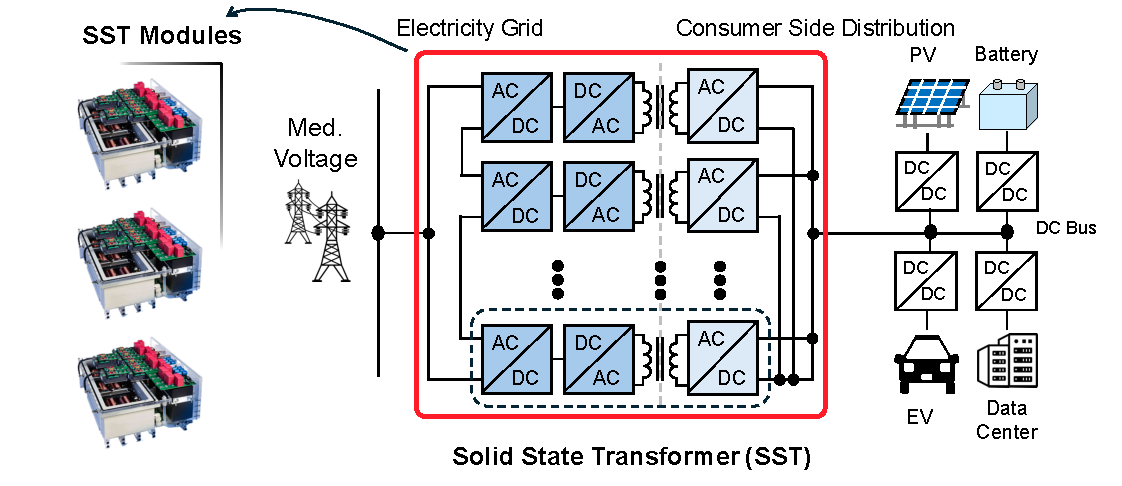
\includegraphics[width=\columnwidth]{figures_intro/SST.pdf}\label{fig:SST}}
\\
     \subfloat[]{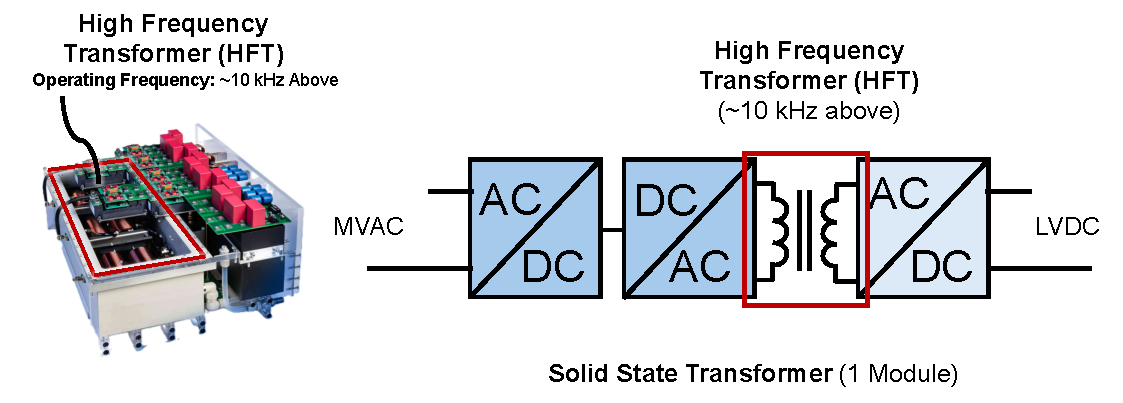
\includegraphics[width=\columnwidth]{figures_intro/module.pdf}\label{fig:module}}
    \caption{Architectures in power distribution: (a) utilizes the Line Frequency Transformer between the MV and LV stage; (b) utilizes the Solid State Transformer (SST) instead with an HFT for galvanic isolation; (c) shows one module of the SST described in (b). The HFT facilitates power transfer from the MV stage to the LV stage. SST Module is from \cite{sstexample} and is included here just for demonstration purposes. LFT is from \cite{lftexample}.}
\end{figure}

The SST is generally characterized by a multi-stage topology \cite{technologies13020074}. To overcome the spatial and weight limitations of line transformers, the SST replaces the massive 50/60 Hz core with a multi-stage architecture comprising wide-bandgap (WBG) semiconductor converters coupled with a high-frequency (HFT) (or medium-frequency (MFT)) isolation transformer. This is most commonly implemented in the isolation stage between the medium-voltage and low-voltage line. A representation of its integration in the power grid is shown in Figure \ref{fig:SST}, and a representation of one module along with the HFT in Figure \ref{fig:module}. The shown representation is just one of the many topologies and applications of the SST and is intended as a general explanatory figure. 

Instead of directly coupling the primary and secondary AC grids using a single magnetic core, the following happens through three main parts connected in series. First, the input AC power (MV) is rectified. Next, a lighter HFT/MFT provides galvanic isolation and voltage stepping. Finally, the output is converted back to DC or AC depending on the application. The mode of conversion for the isolation stage depends on the system configuration or application. To allow for the increase in power generation, as seen in Figure \ref{fig:SST}, the input side of the modules are connected in series to accommodate the MV grid, whereas the output converters are connected in parallel to accommodate higher load currents.

The benefits of SSTs mainly encompass the enabling the broad possibilities of controllability and advanced functions, including but not limited to: reactive power compensation, active filtering, fault handling, its potential for modularity, and the potential for low-voltage DC link for easy integration of various systems. As one of the main goals is to improve power density by replacing the line frequency transformer, then a lot of applications are gaining interest. These include but are not limited to high-power EV charging, future traction applications, data centers, renewable energy applications, and even smart grid systems \cite{10667423}, \cite{6342269}, \cite{8962031}, \cite{czyz2021}. 

As highlighted in recent state-of-the-art reviews of SST technologies, the viability of these systems has been greatly accelerated by the maturity of Silicon Carbide (SiC) and Gallium Nitride (GaN) devices. With semiconductor technology advancing rapidly, research has now shifted towards optimizing the power converter topologies and, most critically, improving the HFT/MFT that form the isolation stage of the SST. 

With the advent of high frequency operation, according to Faraday's Law, operating at elevated frequencies allows the magnetic core area and the number of winding turns to be drastically reduced. This results in a system that offers a fraction of the size and weight of a traditional line transformer while providing enhanced control over bidirectional power flow and fault isolation  \cite{10667423}, \cite{6342269}, \cite{8962031}, \cite{czyz2021}. 

An example is shown in Figure \ref{app:downsizing}. By the Area Product Method, scaling from 60 Hz to 10 kHz can might be able to provide about 98\% reduction in transformer volume, as shown in Figure \ref{fig:downsizing}a.  Details are shown in the Appendix: \nameref{app:downsizing}. But, as a trade-off, with more core and winding losses at higher frequency, thermal management becomes a problem for the HFT, as shown in the example provided in Figure \ref{fig:downsizing}b \cite{downsizing}. 

\begin{figure}
    \centering
    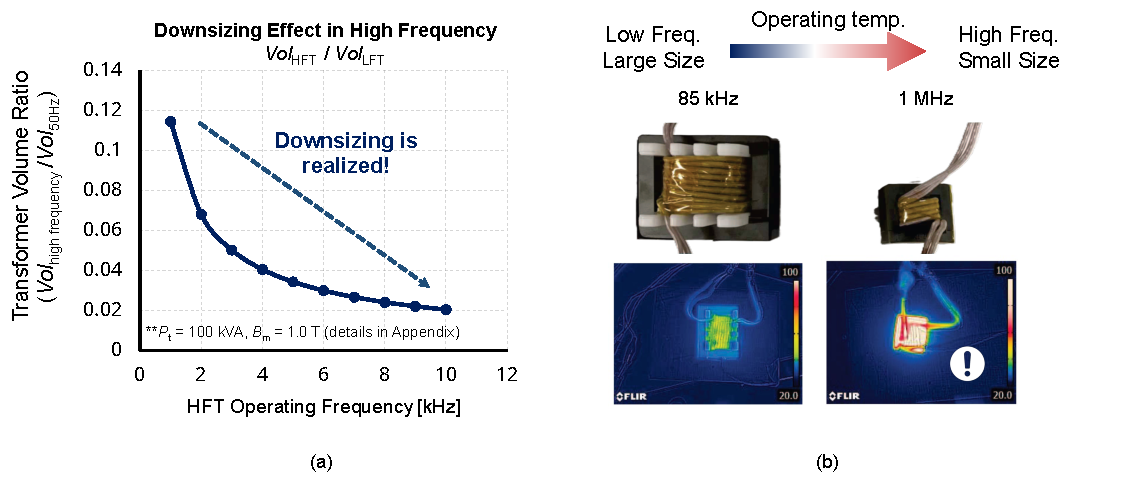
\includegraphics[width=\columnwidth]{figures_intro/downsizing.pdf}
    \caption{Operation at higher frequency brings benefits with a trade-off: (a) downsizing effect from the LFT as an effect of HF operation, details shown in Appendix \nameref{app:downsizing}; (b) thermal management trade-off shown in \cite{downsizing}.}\label{fig:downsizing}
    
\end{figure}

This profound downsizing effect renders solid-state transformers (SSTs) more essential than ever for modern power networks. Traditional line-frequency transformers (LFTs) rely on massive quantities of copper, magnetic materials, and other physical resources, consuming substantial natural resources to construct, transport, and maintain. By transitioning to a high-frequency SST architecture, this physical bulk is drastically mitigated. The resulting reduction in raw volume and weight not only alleviates the strain on global material supply chains but also significantly reduces manufacturing lead times and heavy-lift installation logistics. Furthermore, overcoming strict spatial constraints is increasingly critical for emerging applications where the highly compact footprint of a high-frequency transformer provides a decisive physical and economic advantage. However, the transition has some challenges as will be explained.
\section{Challenges in the Isolation Transformer Design} \label{sec:challenge}
The HFT/MFT in the isolation stage performs the same function as the traditional
50/60 Hz transformer which is to enable voltage transformation and provide electrical isolation between MV/HV and LV sides. However, a key feature is the operation at higher voltages and frequencies. This creates new challenges in the pillars of transformer design:
\begin{itemize}
    \item \textbf{Efficiency}: as explained in the previous section, with higher frequency and voltage operation means the increase of both core and winding losses. Primarily, for core losses, this means the selection of material that will provide high saturation flux density, compatible operating temperature, and low-loss in the desired operation condition \cite{ref1}. For winding losses, this entails careful winding methods to eliminate the effects of skin and proximity losses.
    \item \textbf{Reliability}: The transformer must simultaneously guarantee robust dielectric isolation under high-voltage stress and effectively manage skyrocketing volumetric heat to prevent thermal failure \cite{6d7bedeb4d374ffaa54effc19030ffd3, https://doi.org/10.1049/hve2.12424}.  
\end{itemize}

While dielectric isolation can be addressed by using improved dielectric material or using a thicker isolation material as well, it is important to note that this affects the thermal management performance of the transformer. Therefore, any attempt to further miniaturize the high-power isolation transformer is limited not primarily by electromagnetics, but by the physical inability to extract heat. 

\section{Thermal Management and Assembly Methods for the HFT}\label{sec:cooling}
The thermal management method for the HFT, as it is a critical part of the overall system packaging, heavily influences the final volumetric power density of the SST. To effectively manage skyrocketing volumetric heat and prevent thermal failure under high-voltage stress, various thermal management methods are currently employed in both academic research and industry.

\subsection{Active Cooling}
Active cooling encompasses the use of forced-air or liquid cooling to accelerate convective heat transfer from the transformer to the ambient environment. While highly effective at managing surface temperatures, active cooling introduces a severe penalty to the power density of the system due to the additional required custom fixtures, mounts, or other components to realize the setup. Liquid cooling systems provide superior heat transfer coefficients but require complex plumbing, pumps, and external radiators. Some examples of transformers built for these systems are shown in Figure \ref{fig:activecooling}a, \ref{fig:activecooling}b, and \ref{fig:activecooling}c \cite{leibl2017design}, \cite{chen2018high}, \cite{mogorovic2019100kw}. 

\begin{figure}[h!]
    \centering
    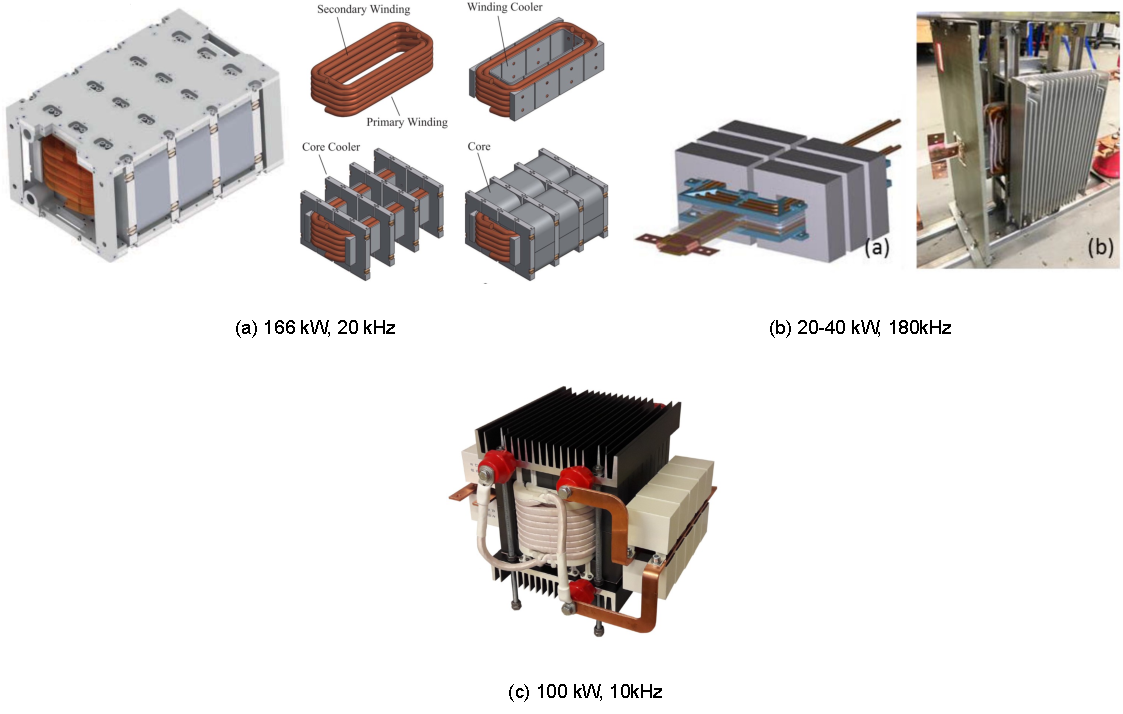
\includegraphics[width=\columnwidth]{figures_intro/forcedair_trans.pdf}
    \caption{Examples of transformers designed for active cooling. (a) is a 166 kW, 20 kHz transformer cooled using liquid cooling \cite{leibl2017design}, (b) is a 20-40 kW, 180 kHz transformer cooled using forced air cooling \cite{chen2018high}, and (c) is a 100 kW, 10 kHz transformer cooled using forced air cooling \cite{mogorovic2019100kw}.}\label{fig:activecooling}
\end{figure}

\subsection{Oil Immersion}
One of the most common methods of thermal management in the high-power domain is the use of oil immersion. While highly effective in both electrical insulation and convective heat transfer, especially when utilizing oil-directed (OD) cooling channels pumped directly through the windings, this method require heavy, bulky sealed tanks, pumps, and external heat exchangers. Furthermore, they introduce significant environmental concerns, maintenance burdens, and flammability hazards, making them undesirable for modern, compact applications \cite{6342269}. Some examples of transformers built for these systems are shown in Figure \ref{fig:oilcooling}a, and Figure \ref{fig:oilcooling}b \cite{anurag2022gen3}, \cite{cremasco2024166kw}. 

\begin{figure}[h!]
    \centering
    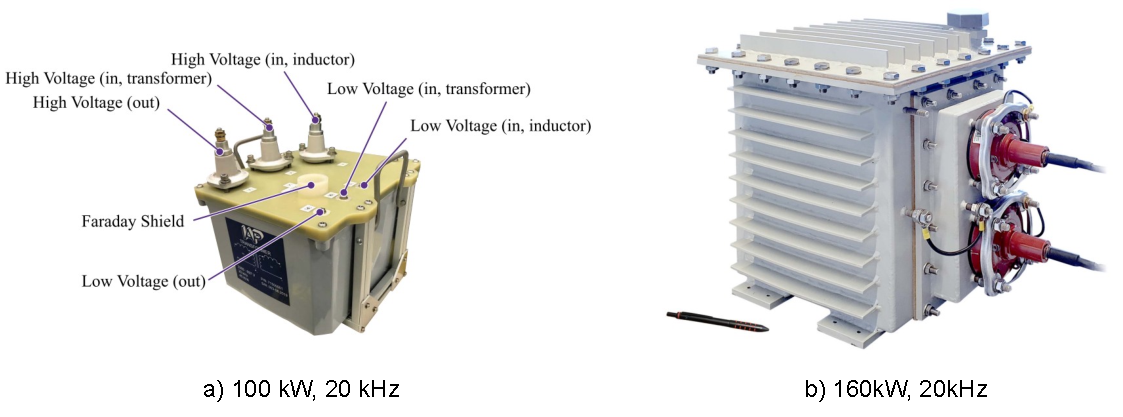
\includegraphics[width=\columnwidth]{figures_intro/oilcooled_trans.pdf}
    \caption{Examples of transformers designed for oil immersion cooling. (a) is a 100 kW, 20 kHz transformer cooled using oil immersion \cite{anurag2022gen3}, and (b) is a 160 kW, 20 kHz transformer cooled using ester oil immersion \cite{cremasco2024166kw}.}\label{fig:oilcooling}
\end{figure}

\subsection{Dry Casting}
To avoid the drawbacks of oil, dry-type medium-frequency transformers heavily rely on epoxy resin dry casting. Vacuum-cast epoxy provides exceptional, partial-discharge-free medium-voltage insulation and structural rigidity, completely encapsulating the core and windings. However, a major fundamental drawback of dry casting is thermal resistance. Standard epoxy resins possess a relatively low thermal conductivity compared to the copper windings they encase. Consequently, the potting material inherently creates a severe thermal barrier, requiring carefully designed cooling systems. Some examples of transformers utilizing this technique is shown in Figure \ref{fig:drycast}a, and \ref{fig:drycast}b \cite{yi2022design}, \cite{gradinger2017novel}. 

\begin{figure}[h!]
    \centering
    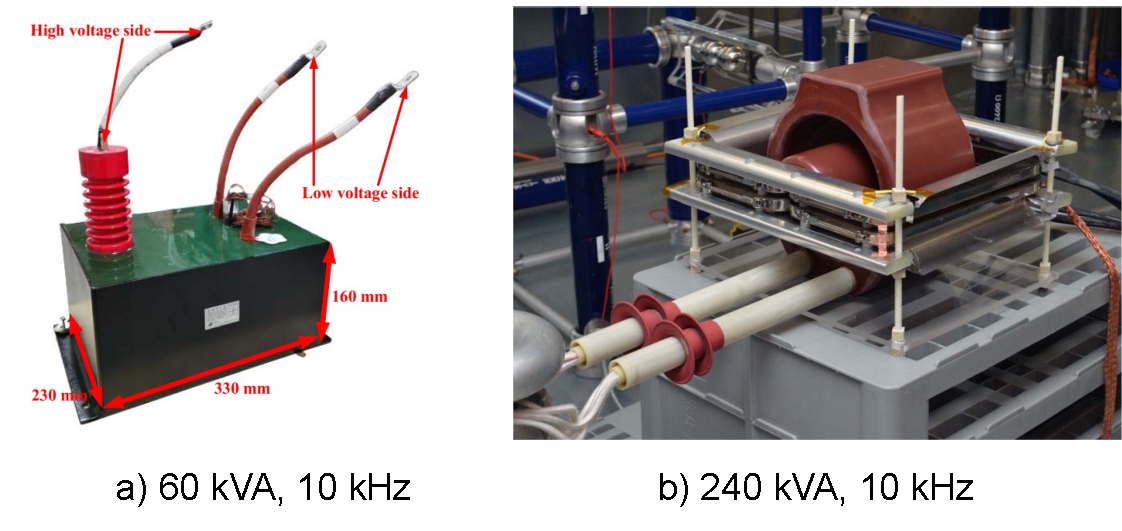
\includegraphics[width=0.7\columnwidth]{figures_intro/drycast_trans.pdf}
    \caption{Examples of transformers assembled using dry casting. (a) is a 60 kVA,10 kHz transformer \cite{yi2022design}, and (b) is a 240 kVA, 10 kHz \cite{gradinger2017novel}.}\label{fig:drycast}
\end{figure}

\subsection{Custom-designed Components}
To circumvent the limitations of standard cooling methods, some researchers utilize the design or insertion of custom components to improve the performance of active cooling or improve internal heat conduction. For instance, optimized 3D-printed bobbins to facilitate specific cooling channels, improving the overall power density by guiding air directly through the core window \cite{ref8, ref9}. Another example involves adding a metal plate in between the ferrite cores to improve heat conduction from the internal core structure into the external heat sink, bypassing the poor thermal conductivity of the ferrite material itself \cite{ref10}. Aside from being highly customized and complex to manufacture, these component-level additions primarily address core heat or surface airflow. They do not fundamentally resolve the geometric winding bottlenecks trapping heat deep within the copper layers.

\begin{figure}[h!]
    \centering
    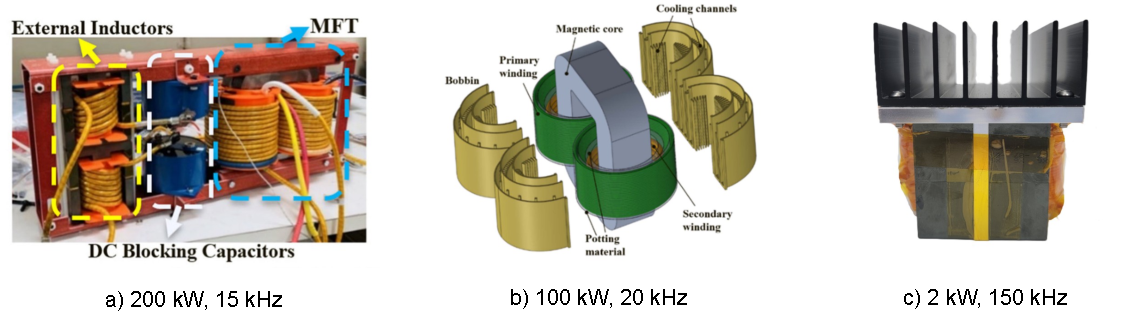
\includegraphics[width=\columnwidth]{figures_intro/custom_trans.pdf}
    \caption{Examples of transformers designed with custom components integrated, and used with other cooling systems: (a) is a 200 kW, 15 kHz transformer \cite{ref8} and (b) is a 100 kW, 20 kHz transformer that both utilize custom designed bobbins for optimized forced air cooling \cite{ref9}, and (c) is a 2 kW, 150 kHz transformer utilizing metal plates sandwiched in between cores for enhanced heat extraction \cite{ref10}.}\label{fig:customtrans}
\end{figure}

It is important to note that the design of cooling and assembly systems for transformers depend on the specific requirements and applications, thus there is no best design for the transformer. While these external and material-based thermal management methods are necessary, addressing the conflict at the foundational geometric level is a promising research direction and has not been currently examined in detail. It presents a highly promising and necessary solution for next-generation SSTs as a potential to reduce dependence on additional thermal management systems. 

\section{The Concept of a Transformer for Improved Intrinsic Thermal Management}
These transformers often use Litz wire to accommodate high current while reducing AC losses at higher frequencies. However, the poor thermal conductivity and low fill factor of Litz wire create a fundamental thermal bottleneck, hindering effective heat extraction \cite{ref11}, \cite{ref12}, which in turn forces a reliance on the aforementioned bulky and complex external cooling systems.

This work therefore investigates a contrasting design approach that prioritizes intrinsic thermal performance of the transformer. Rectangular windings are known to offer advantages like high current capacity and excellent fill factor, and they are applied as well to inductors \cite{ref22}, \cite{ref23}. However, a characterization of their thermal properties in the specific context of transformers is limited. Additionally, most of the transformers presented in the previous discussion do not use a planar structure. 

To address this, a low-profile planar structure is proposed that utilizes solid rectangular conductors arranged in a flatwise orientation, as shown in Figure \ref{fig:concept_trans}, with its cross-sectional area view in \ref{fig:concept_cross}. This geometric arrangement creates highly effective, parallel thermal paths for direct heat extraction from every turn. The details are further explained in Chapter 3 of this paper.

\begin{figure}[h!]
    \centering
    \subfloat[]{
    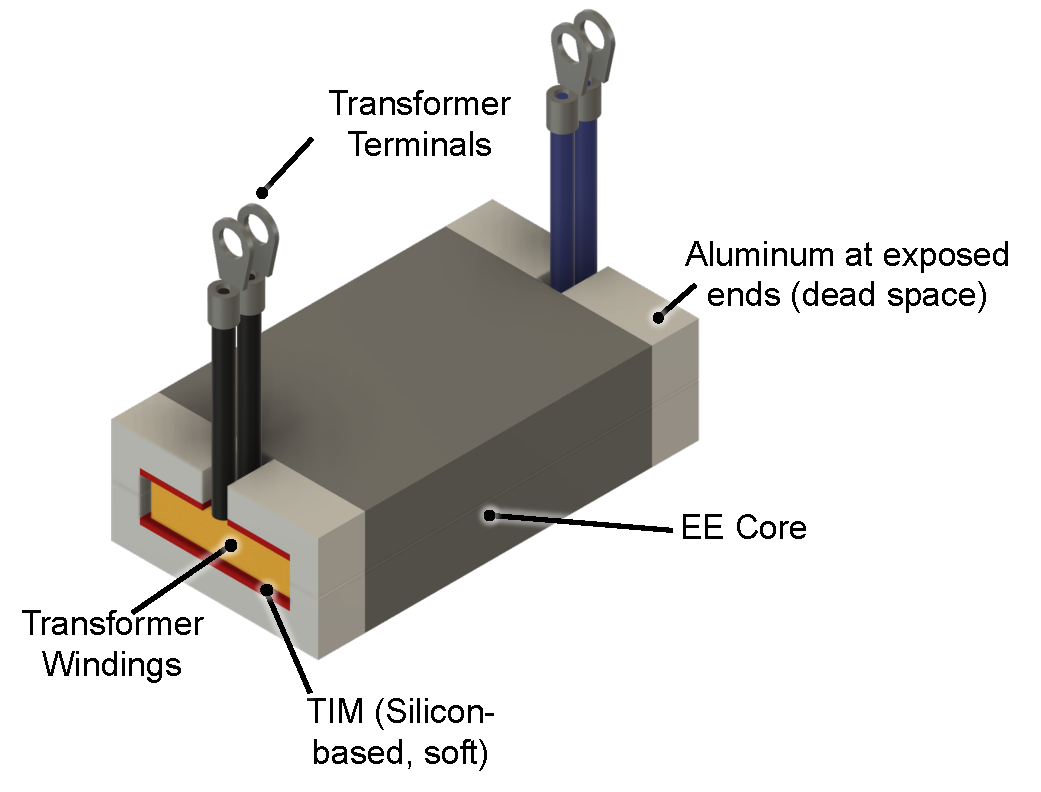
\includegraphics[width=0.6\columnwidth]{figures_intro/concept.pdf}\label{fig:concept_trans}
    }
    \subfloat[]{
    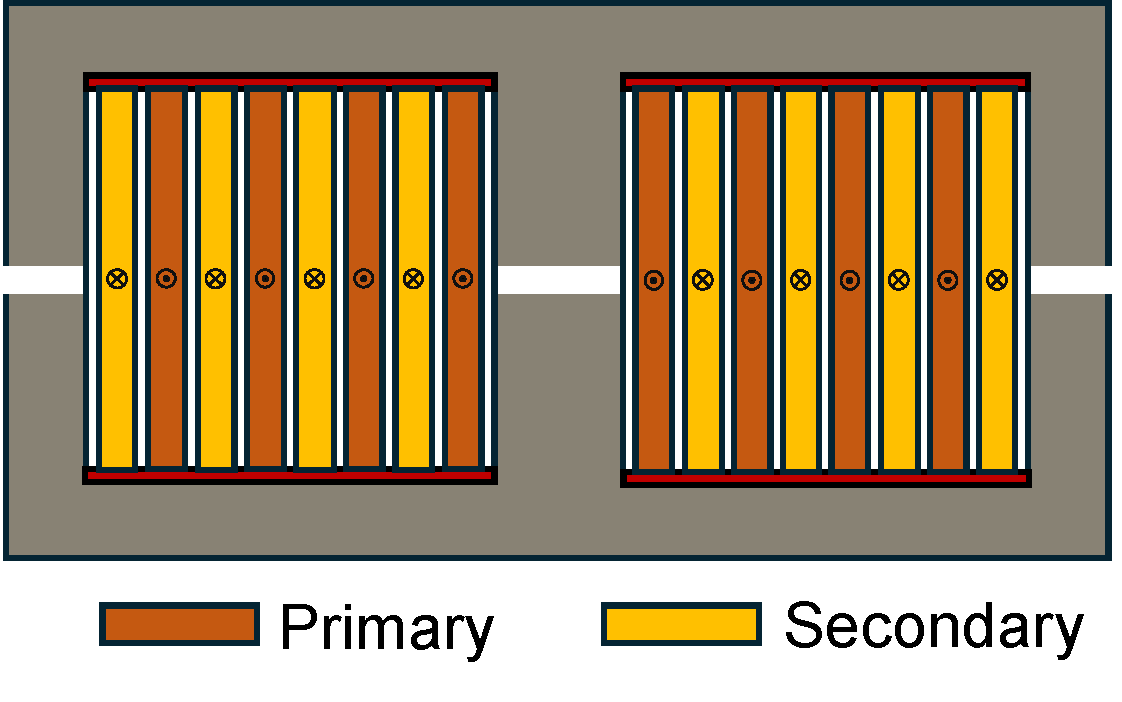
\includegraphics[width=0.4\columnwidth]{figures_intro/concept_cross.pdf}\label{fig:concept_cross}
    }
    \caption{Representative model of an flatwise-wound transformer: (a) mockup of the transformer, and (b) cross-sectional view of the transformer.}
\end{figure}

\section{Objectives of the Study}
\par This study has three main goals. Firstly, this study aims to propose a novel flatwise-wound planar transformer geometry that establishes the internal heat extraction from a restrictive series path to a highly conductive parallel path. Important parameters, such as the AC winding losses, core losses, and magnetizing inductance, are examined to properly optimize the physical dimensions of the transformer. A 1D Thermal Network is also proposed to qualitatively examine the heat extraction mechanism of the proposed flatwise structure. Secondly, this study aims to confirm the feasibility and thermal superiority of the proposed transformer in comprehensive 3D Multi-Physics Finite Element Analysis (FEA). The uniform heat distribution and the elimination of the series thermal bottleneck are confirmed in simulation. Lastly, this study aims to experimentally verify the thermal stability offered by the proposed flatwise design. A continuous full-load operational comparison against its conventional,edgewise-wound counterpart is also performed in this study. The advantage of the proposed configuration is also compared both in simulation and experiment to its conventional counterpart. The concept is proven with a 1-kW, 100V:100 V, 28.5-kHz bidirectional CLLC resonant converter, which is the small-scale counterpart of its high-power 100 kW, 1000V:1000V CLLC for the isolation stage of the SST. 

\section{Significance of the Study}
\par This study is expected to contribute significantly to the existing field of high-power isolation transformers for SST applications. The geometric method presented in this study improves the intrinsic thermal management of the transformer, thereby reducing the dependence on active cooling systems and unlocking higher limits for volumetric power density. Furthermore, while extensive research exists on optimizing the electrical parameters of planar magnetics, studies specifically focusing on the internal thermal path packaging and physical layout optimization are less common. This research directly contributes to bridging the gap between electromagnetic performance and mechanical thermal reliability. Lastly, as a scalability analysis was performed, it provides a lot of insights as to what could be done in future iterations of this work.
\section{Flow of the Paper}
The flow of the paper is structured as follows:
\begin{itemize}
\item \textbf{Chapter 2} presents the motivations behind the selection of the application circuit, which is the bidirectional CLLC resonant converter. It defines the industrial system specifications, the operational modes and adaption to a small-scale study.
\item \textbf{Chapter 3} details the design methodology of the proposed flatwise-wound transformer. It establishes the intrinsic thermal management concept through 1D thermal models, and the analytical equations used to design the transformer.
\item \textbf{Chapter 4} examines the proposed transformer through 3D FEA multi-physics simulations, providing a direct thermal and electrical comparison between the flatwise and conventional edgewise geometries.
\item \textbf{Chapter 5} presents an experimental comparison. A 1 kW proof-of-concept comparison between the proposed flatwise-wound and conventional edgewise-wound structure is evaluated using a representative model with a square window area under continuous operation.
\item \textbf{Chapter 6} presents a conservative, thermal scalability analysis in terms of spatial geometry and operational power. The analysis in Chapter 4 is extended to examine how the thermal benefit of the proposed configuration performs in different spatial profiles and its potential to operate at higher power levels has been examined. 
\item \textbf{Chapter 7} provides the conclusions drawn from the present status of the work and outlines recommendations for future research prospects.
\end{itemize}

\section{About This Work}
This research project is performed in collaboration with ABB Oy and HighQ Power Oy to meet next-generation industrial power conversion demands.

Portions of this study were presented at the \textit{IEEE Applied Power Electronics Conference and Exposition (APEC)}, held in San Antonio, Texas, USA in March 2026. The content included in that presentation focuses primarily on the analytical design and thermo-electromagnetic simulation discussed in Chapter 3 and Chapter 4.

Furthermore, more findings from this work were presented at the \textit{International Conference on Materials and Systems for Sustainability (ICMaSS)} held in Nagoya, Japan in December 2025 and the \textit{IEEE International Power Electronics Conference (IPEC)}, held in Nagasaki, Japan in June 2026. The content of those presentations focuses on the geometric thermal analysis detailed in Chapter 4 and the experimental comparison presented in Chapter 5.




\chapter{Application Topology Selection and Design}
The design of high-frequency magnetic components is strictly dictated by the electrical specifications of the target power conversion system. This research is driven by demands for high-power, high-frequency SSTs and other applications that require the said architecture, which includes fast-charging infrastructure and energy distribution systems. This chapter details insights regarding the selection of the application topology for the proposed isolation transformer.

\section{System Specifications}
Based on the established research demands, the target electrical parameters for the isolation stage DC--DC converter are as shown in Table \ref{tab:converter_specs}. Operating within these regimes requires a converter topology that can minimize switching losses while accommodating the isolation stage transformer.

\begin{table}[h!]
\centering
\caption{Established Converter Specifications}
\label{tab:converter_specs}
\begin{tabular}{cccc}
\hline
\textbf{Parameter} & \textbf{Symbol} & \textbf{Value} \\
\hline \hline
Input Voltage & $V_{\mathrm{in}}$ & nom. 1000 V \\ 
Output Voltage & $V_{\mathrm{out}}$ & 1000 V   \\
Switching Frequency & $f_{\mathrm{sw}}$ & 15 -- 30 kHz \\ 
Output Power & $P_\mathrm{O}$ & 100 kW \\
Output Current & $I_\mathrm{O}$ & 100 A \\
\hline
\end{tabular}
\end{table}

In this study, due to the capabilities of the researchers and laboratory, and especially that the research first requires a proof of concept, a scaled down version of the system is first examined, equally scaling down current and voltage by 10 each to reach a baseline nominal operating condition of 100 V: 100 V, 1 kW, under the same operating frequency condition. The transformer turn ratio $n$ is set to 1.

\section{Considered High Power Topologies}
In SST applications, most topologies should have bidirectional capability to allow interoperation between the grid and its consumers. Selecting the optimal isolated bidirectional DC--DC converter topology is a critical first step, and most topologies in this application use the Dual Active Bridge (DAB) Converter and the Capacitor-Inductor-Inductor-Capacitor (CLLC) resonant converter. Their circuit diagrams are shown in Figure \ref{fig:DAB} and Figure \ref{fig:CLLC}. 

\begin{figure}[h!]
    \centering
    \subfloat[]{
        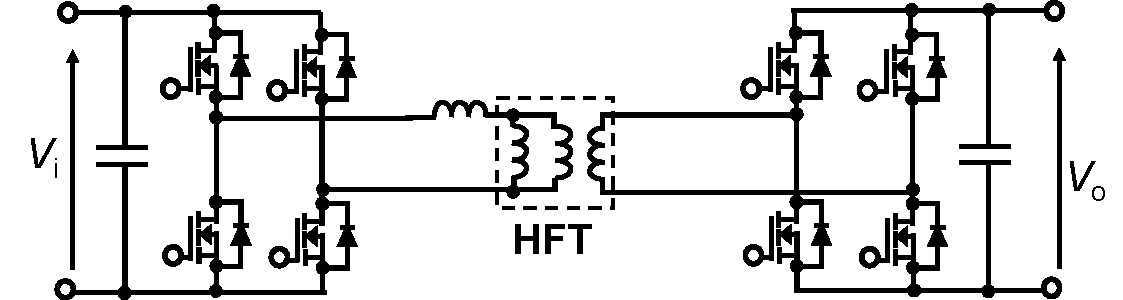
\includegraphics[width=0.8\columnwidth]{figures_chapter2/DAB.pdf} \label{fig:DAB}
    }
\\
     \subfloat[]{
        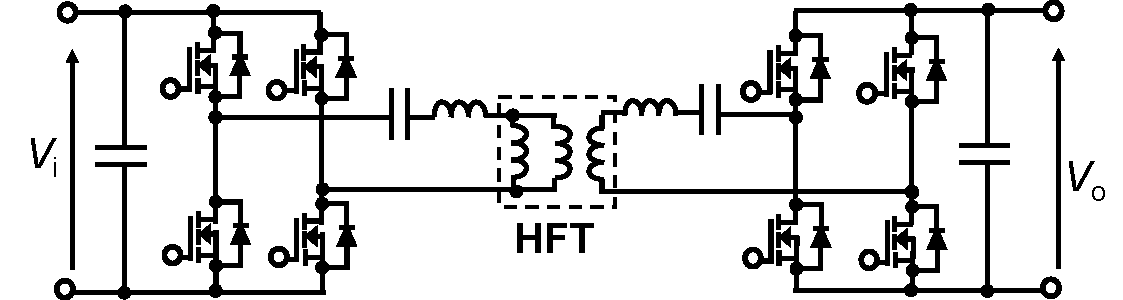
\includegraphics[width=0.8\columnwidth]{figures_chapter2/CLLC.pdf} \label{fig:CLLC}
    }
\caption{Bidirectional converters for SST applications: (a) the Dual Active Bridge (DAB) converter, and (b) the Capacitor-Inductor-Inductor-Capacitor (CLLC) resonant converter.}
\end{figure}


\begin{figure}[H]
    \centering
    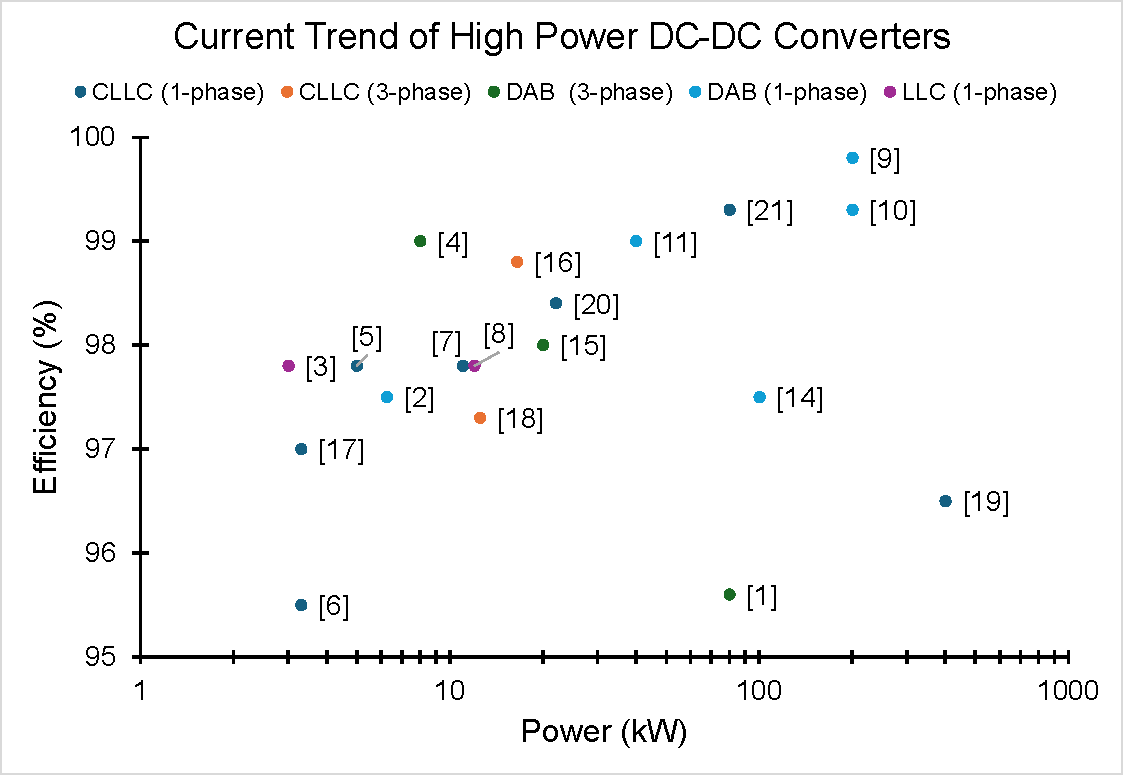
\includegraphics[width=0.8\columnwidth]{figures_chapter2/HighPower.pdf}
    \caption{A compilation of high power converters at different power levels. The data utilized can be seen in the Appendix: \nameref{app:converter_trends}.}\label{fig:HighPower}
\end{figure} 
A compilation of the current trend of high-power converters is shown in Figure \ref{fig:HighPower}. Most high power converters in SST Applications utilize the DAB. This is due to their versatility and ease of operation and control. However, the DAB is prone to DC Bias due to the control scheme used \cite{zhang2019analog}. Eliminating DC Bias is important as it can resolve to core saturation, which can then cause excessive heating, loss, and disruption to circuit operation. Moreover, it is also known to have a narrow ZVS range and higher peak current when the phase shift increases, leading to more losses \cite{krismer2012efficiency}. 

To overcome these limitations, the bidirectional CLLC resonant converter is selected for this study. The CLLC topology integrates a symmetric resonant tank on both the primary and secondary sides of the high-frequency transformer. It is also known to have a wider range of ZVS operation even at lighter loads, which can improve efficiency in the overall operating range. It utilizes resonance and the magnetizing inductance to store and transfer energy through the fine tuning of operation frequency. However, it is difficult to implement frequency control, and careful tuning of the two resonant tanks. Moreover, higher peak operational current is expected, which can cause more component stress \cite{ref19, mukherjee2021comparison}. 

A short summary comparing each topology is shown in Table \ref{tab:tabcomparison}. 

\begin{table}[h!]
\centering
\caption{Comparison of DAB and CLLC Resonant Converters \cite{mukherjee2021comparison, oh2024comparison}} \label{tab:tabcomparison}
\label{tab:dab_vs_cllc}
\begin{tabular}{
    >{\raggedright\arraybackslash}p{0.22\textwidth} 
    >{\raggedright\arraybackslash}p{0.35\textwidth} 
    >{\raggedright\arraybackslash}p{0.35\textwidth}
}
\hline
\textbf{Parameter} & \textbf{Dual Active Bridge Converter \cite{krismer2012efficiency, costa2015modular, anwar2018modeling}} & \textbf{CLLC Resonant Converter \cite{ref19, xie2019analysis}} \\
\hline \hline

\textbf{Efficiency} & 
Peak efficiency is achieved near nominal load; efficiency degrades significantly under light loads due to circulating currents. & 
Maintains high efficiency across a substantially wider load range due to minimized switching and circulating losses. \\

\textbf{Control Strategy} & 
Phase-Shift Modulation (PSM); conceptually straightforward but requires highly precise timing synchronization between bridges. & 
Pulse Frequency Modulation (PFM); regulates voltage gain effectively without relying on complex cross-isolation communication. \\

\textbf{Soft-Switching (ZVS)} & 
ZVS region is constrained; often lost under light-load conditions or non-unity voltage gains. & 
Inherent ZVS capability is maintained seamlessly across a wide operating region for both forward and reverse power flow. \\

\textbf{Current Characteristics} & 
Trapezoidal current profile; minimizes RMS currents only when operating under optimal, low phase-shift conditions. & 
Sinusoidal current profile; inherently results in higher RMS currents compared to an optimized DAB. \\

\textbf{Component Stress} & 
High circulating reactive currents and elevated core losses when operating away from the optimal design point. & 
Higher peak operational currents impose stricter thermal and electrical stress ratings on semiconductor devices. \\

\textbf{Component Count \& Complexity} & 
8 switches and 1 series transfer inductor (typically integrated utilizing the transformer's leakage inductance). & 
8 switches, plus primary and secondary resonant capacitors. Sourcing AC capacitors for high-voltage/high-current ratings can increase volume and cost. \\

\textbf{Target Applications} & 
Ideal for fixed-voltage-ratio (DCX) applications prioritizing maximum full-load density and efficiency. & 
Ideal for bidirectional applications requiring wide input/output voltage regulation (e.g., EV chargers, SSTs). \\

\hline
\end{tabular}
\end{table}
\pagebreak
\section{The Bidirectional Resonant Converter}
\subsection{CLLC Operational Mode Analysis}
The bidirectional CLLC resonant converter operates through distinct topological states during each switching half-cycle \cite{infineon_cllc, ref19}. In this explanation, operation is assumed at or near the resonant frequency. Moreover, for brevity, the operational analysis is performed only for the first pair of switches, $S_1$ and $S_4$, operating in forward power delivery. This then means that the secondary side switches are off and are in rectification operation. The process is symmetrical for the other pair of switches, and also for reverse power delivery. An illustration of the first three modes of operation is shown in Figure \ref{fig:operation} and the key waveforms are shown in Figure \ref{fig:keywaveform}.
\begin{figure}[h!]
    \centering
    \subfloat[]{
        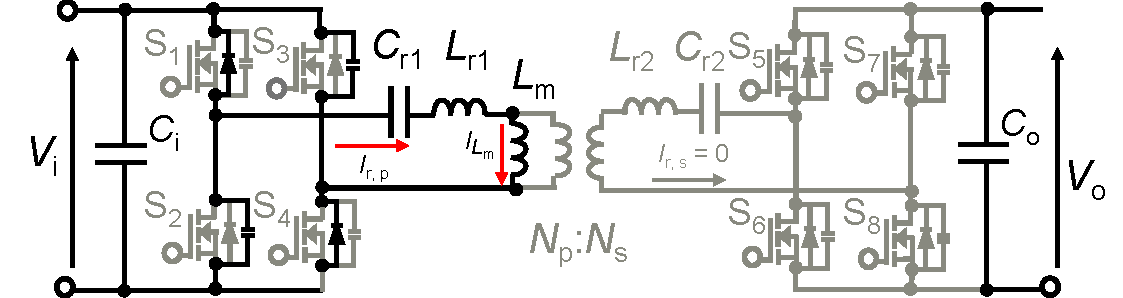
\includegraphics[width=0.8\columnwidth]{figures_chapter2/mode1.pdf} \label{fig:mode1}
    }
\\
     \subfloat[]{
        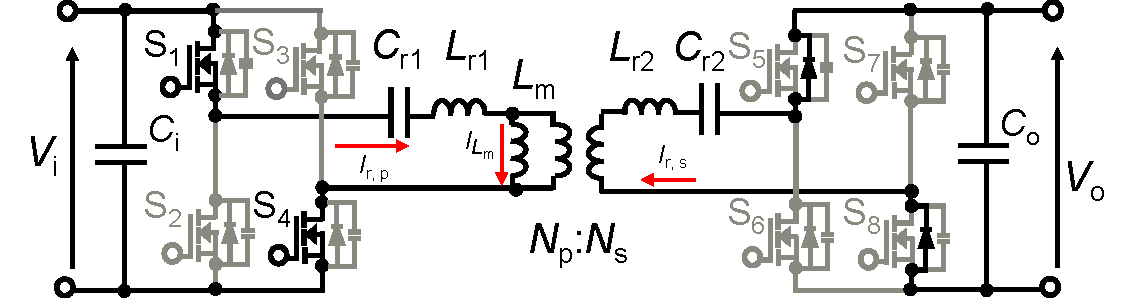
\includegraphics[width=0.8\columnwidth]{figures_chapter2/mode2.pdf} \label{fig:mode2}
    }
\\
     \subfloat[]{
        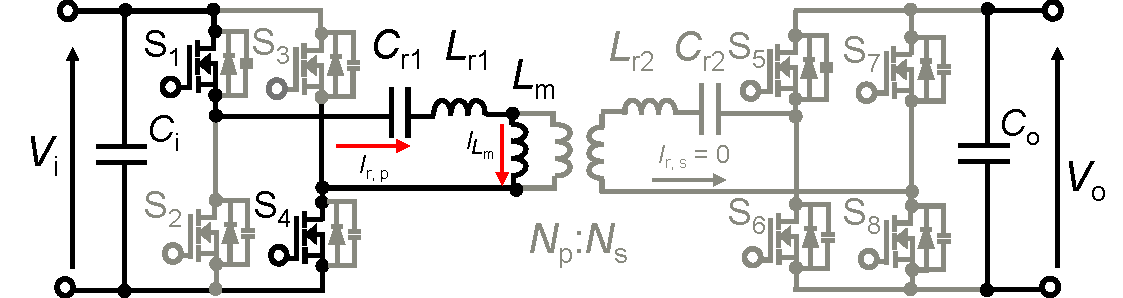
\includegraphics[width=0.8\columnwidth]{figures_chapter2/mode3.pdf} \label{fig:mode3}
    }
\caption{First three modes of operation of the CLLC: (a) State 1 $t_1<t<t_2$, (b) State 2 $t_2<t<t_3$, and (c) State 3 $t_3<t<t_4$.} \label{fig:operation}

\end{figure}

\begin{figure}[h!]
    \centering
    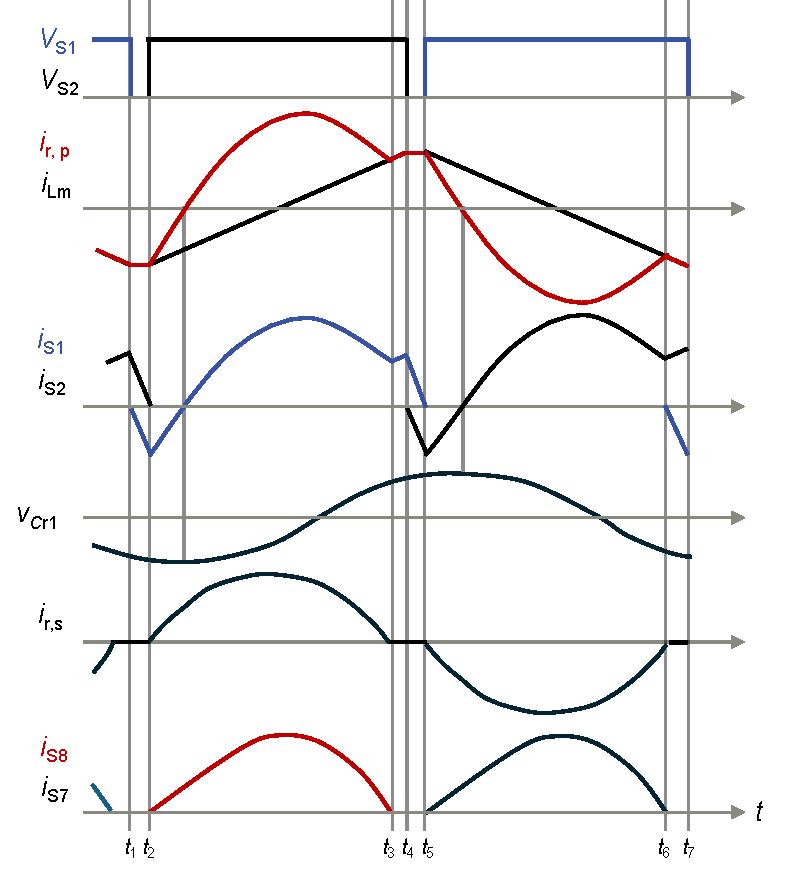
\includegraphics[width=0.8\columnwidth]{figures_chapter2/operational waveform.pdf}
\caption{Key waveforms of the CLLC.}\label{fig:keywaveform}
\end{figure}

\textbf{State 1 (Dead Time), $t_1<t<t_2$} (Figure \ref{fig:mode1}) :
All switches are off to avoid overshoot. During the dead-time duration, no power is transferred to the secondary side. The primary resonance current $i_\mathrm{r, p}$ charges the output capacitances of switches $S_2$ and $S_3$ and discharges those of $S_1$ and $S_4$. After this process, $i_\mathrm{r,p}$ will pass through the diode of $S_1$ and $S_4$, which signifies ZVS.

\textbf{State 2 (Power Transfer Stage),  $t_2<t<t_3$} (Figure \ref{fig:mode2}):
Switches $S_1$ and $S_4$ turn on, enabling power transfer through the transformer. The primary side resonance current $i_\mathrm{r,p}$ changes direction, and the magnetizing inductance stores energy, as $i_{\mathrm{Lm}}$ rises linearly. This stage ends when $i_\mathrm{p}$ meets $i_\mathrm{Lm}$, signifying the end of the resonance operation.

\textbf{State 3 (Freewheeling State), $t_3<t<t_4$} (Figure \ref{fig:mode3}):
Because resonance operation is stopped, $i_\mathrm{r, s}$ is zero. This therefore means that $i_\mathrm{r, p}$ is also the same as $i_\mathrm{Lm}$, storing energy into the magnetizing inductance until $S_1$ and $S_4$ are turned off. When $L_\mathrm{m}$ is large enough, $i_\mathrm{r, p}$ follows $i_{\mathrm{Lm}}$ perfectly.

\subsection{CLLC First Harmonic Approximation (FHA)} \label{ref:FHA}
The First Harmonic Approximation (FHA) is a widely adopted analytical method for deriving the voltage gain and tuning the resonant tank parameters of the CLLC converter \cite{ref19}, \cite{infineon_cllc}. Because the resonant tank acts as a highly effective bandpass filter, the FHA method assumes that power transfer is overwhelmingly dominated by the fundamental harmonic component of the square-wave voltage generated by the active bridge. This then allows the circuit to be converted to an equivalent circuit with a sinusoidal input voltage and output as well. The equivalent input voltage $V_\mathrm{in, app}$, $V_\mathrm{o, app}$, and equivalent AC current $I_{\mathrm{ac}}$ are mapped out in both the original and equivalent circuit as shown in Figure \ref{fig:AC_orig} and Figure \ref{fig:AC_eq} respectively. The  AC resistance $R_{\mathrm{ac}}$ is the equivalent of the DC load with current $I_{\mathrm{o}}$ passing through it.

\begin{figure}[h!]
    \centering
    \subfloat[]{
        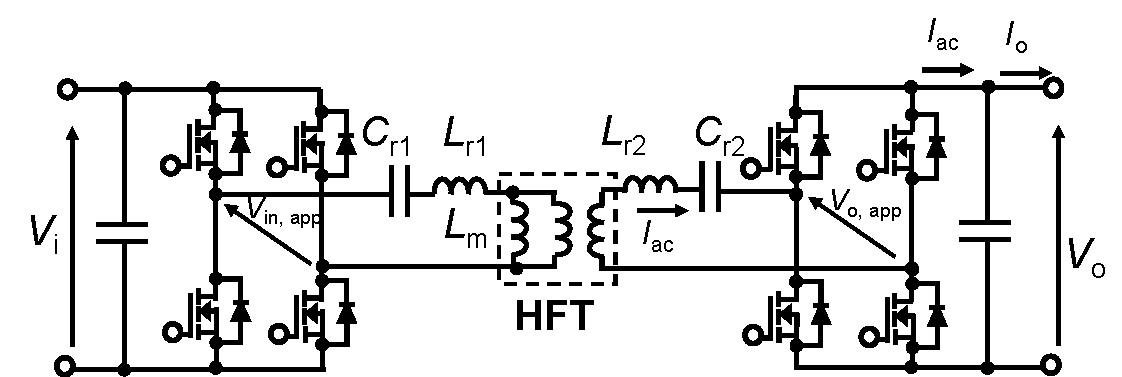
\includegraphics[width=0.9\columnwidth]{figures_chapter2/CLLC_FHA_full.pdf} \label{fig:AC_orig}
    }

     \subfloat[]{
        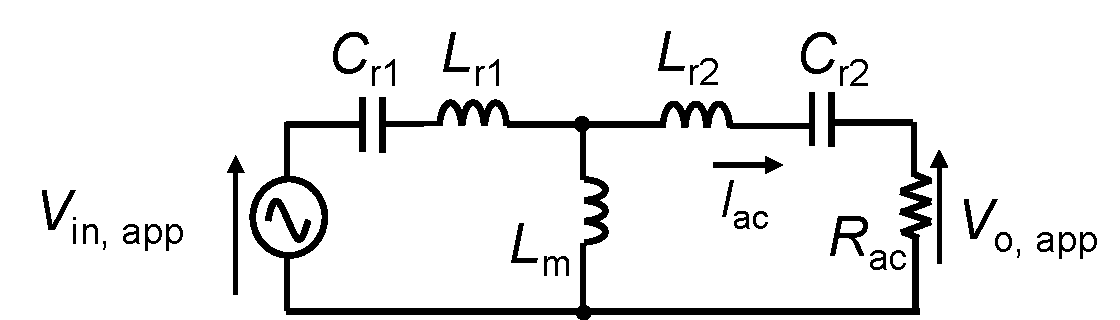
\includegraphics[width=0.7\columnwidth]{figures_chapter2/FHA_Equivalent.pdf} \label{fig:AC_eq}
    }
\caption{First Harmonic Analysis: (a) original circuit, (b) equivalent circuit after FHA.}
\end{figure}

By applying a Fourier series expansion, the fundamental component of the input square-wave voltage $V_{\mathrm{in, app}}(t)$ is extracted as shown in Eq. \ref{eq:fha_vs}:
\begin{equation}
V_{\mathrm{in, app}}(t) = \frac{4}{\pi}V_{\mathrm{in}}\sin(\omega t)
\label{eq:fha_vs}
\end{equation}

The other quantities $V_{\mathrm{out, app}}(t)$, $I_{\mathrm{ac}}(t)$, and $I_{\mathrm{ac}}(rms)$  follow as below, given that $n=1$:
\begin{align}
    V_{\mathrm{out,app}}(t) &= \frac{4V_{\mathrm{in}}}{\pi} \sin(\omega t - \phi) = \frac{4V_{\mathrm{o}}}{\pi}\sin(\omega t - \phi)\\
    I_{\mathrm{ac}}(t) &= \sqrt{2}I_{\mathrm{ac,rms}} \sin(\omega t - \phi) \\
    I_{\mathrm{ac,rms}} &= \frac{\pi}{2\sqrt{2}}I_o
\end{align}

The equivalent AC resistance $R_\mathrm{ac}$ can be expressed by the DC load as follows in Eq. \ref{eq:Rac}:
\begin{equation}
R_{\mathrm{ac}} = \frac{V_{\mathrm{out,app,rms}}}{I_{\mathrm{ac,rms}}} = \frac{8}{\pi^2} \frac{V_O}{I_O} = \frac{8}{\pi^2} R_O \label{eq:Rac}
\end{equation}

The voltage gain $\mathbf{M}_g$ can be obtained from the equivalent circuit in Figure \ref{fig:AC_eq}, denoting $C_{\mathrm{r1}}$ and $L_{\mathrm{r1}}$ as $\mathbf{Z}_1$, $C_{\mathrm{r2}}$ and $L_{\mathrm{r2}}$ as $\mathbf{Z}_2$, and $L_\mathrm{m}$ as $\mathbf{Z}_3$ as shown in Eq. \ref{eq:gain}. It is also important to note that since $n=1$, the resonant tank elements are symmetric for the primary and secondary sides.

\begin{equation}
\mathbf{M}_g(s) = \frac{\mathbf{V_\mathrm{o, app}}(s)}{\mathbf{V_\mathrm{i, app}}(s)} = \frac{\mathbf{V_\mathrm{o}}(s)}{\mathbf{V_\mathrm{in}}(s)} = \frac{(\mathbf{Z}_2 + R_{\mathrm{ac}}) \parallel \mathbf{Z}_3}{\mathbf{Z}_1 + [\mathbf{Z}_3 \parallel (\mathbf{Z}_2 + R_{\mathrm{ac}})]} \cdot \frac{R_{\mathrm{ac}}}{\mathbf{Z}_2 + R_{\mathrm{ac}}}\label{eq:gain}
\end{equation}

The following quantities are introduced as these relate the parameters of the resonant tank, transformer, and the circuit to the voltage gain:
\begin{itemize}
\item The inductance ratio $k$ is defined as the ratio of the magnetizing inductance to the primary resonant inductance, denoted as $k = L_\mathrm{m}/L_\mathrm{r1}$.
\item The quality factor $Q$ is defined as the  characteristic impedance of the resonant tank relative to the load, denoted as $Q = \frac{\sqrt{L_\mathrm{r1}/C_\mathrm{r1}}}{R_\mathrm{ac}}$.
\item The normalized frequency $f_n$ is the ratio between the switching frequency $f_\mathrm{sw}$ and the resonant frequency $f_\mathrm{r}$, denoted as $f_n = \frac{f_\mathrm{sw}}{f_\mathrm{r}}$.
\item The resonance frequency $f_\mathrm{r}$ is the frequency at whcih $M_g = 1$. It can be denoted in terms of the resonant tank as $f_\mathrm{r} = \frac{1}{2\pi \sqrt{L_\mathrm{r1} \cdot C_\mathrm{r1}}}$.
\end{itemize} 

The gain indicated in Eq. \ref{eq:gain} can be then rewritten in terms of the introduced quantities as  shown in Eq. \ref{eq:newgain}:
\begin{equation}
\|M_g(j\omega)\| = \frac{V_\mathrm{o}}{V_\mathrm{in}}=\frac{1}{\sqrt{\left( Q f_{\mathrm{n}} \left( \frac{1}{k} + 2 \right) - \frac{Q}{f_{\mathrm{n}}} \left( \frac{2}{k} + 2 \right) + \frac{Q}{k f_{\mathrm{n}}^3} \right)^2 + \left( \frac{1}{k} - \frac{1}{k f_{\mathrm{n}}^2} + 1 \right)^2}}\label{eq:newgain}
\end{equation}

The gain curve can be shaped by choosing a value for $k$ and $Q$ over $f_n$ which can in turn then give the resonant parameters for the circuit. Shown in Figure \ref{fig:constantQ} is a gain curve shaped by $k$ and in Figure \ref{fig:constantK} is a gain curve shaped by $Q$.

\begin{figure}[h!]
    \centering
    \subfloat[]{
        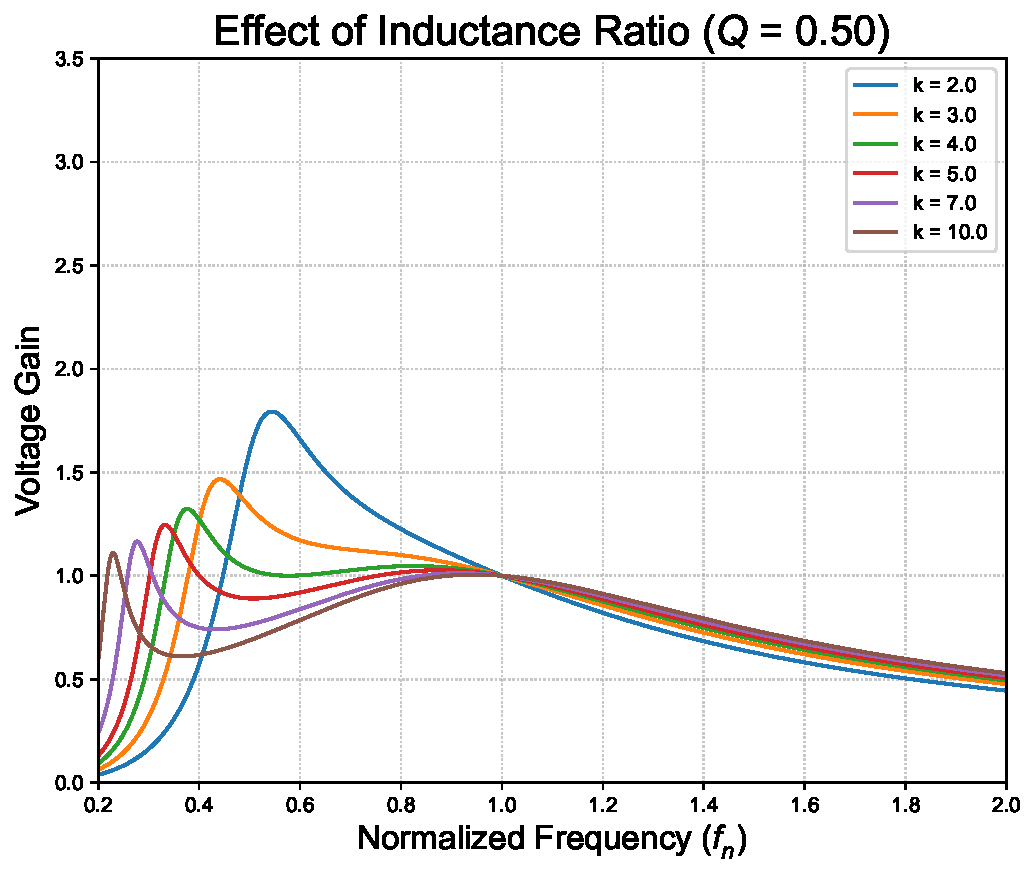
\includegraphics[width=0.5\columnwidth]{figures_chapter2/effect_of_k.pdf} \label{fig:constantQ}
    }
     \subfloat[]{
        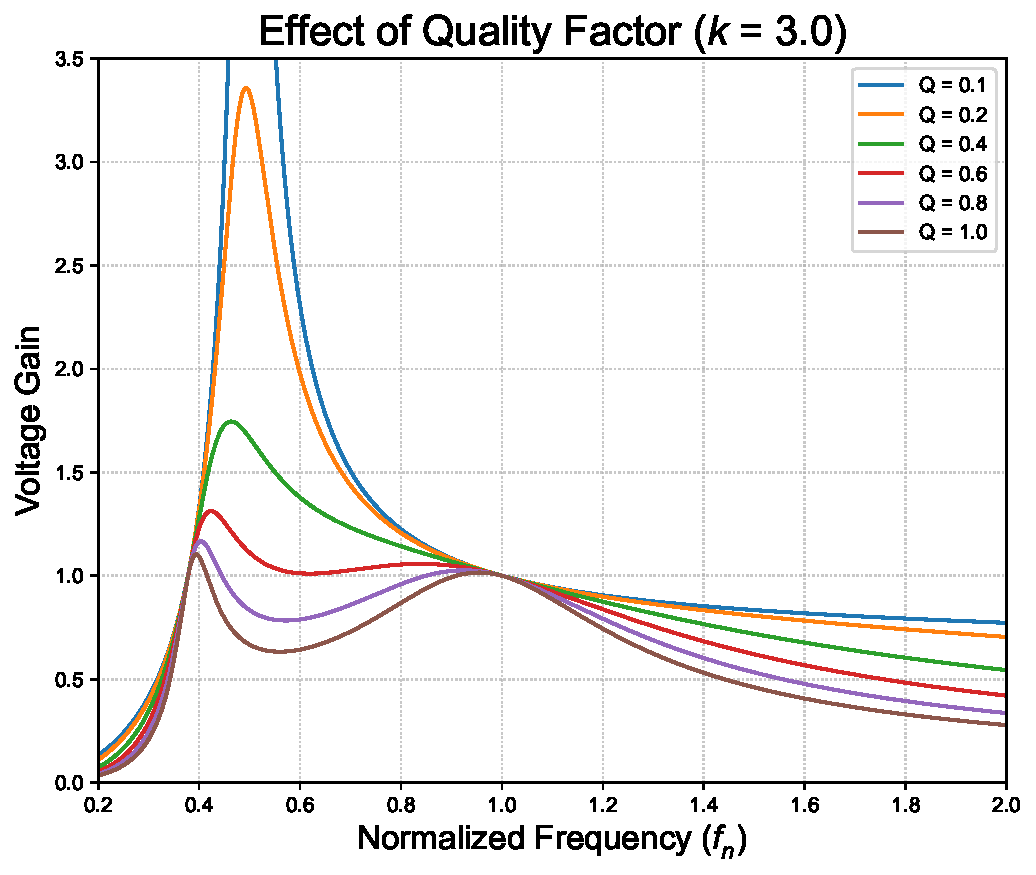
\includegraphics[width=0.5\columnwidth]{figures_chapter2/effect_of_Q.pdf} \label{fig:constantK}
    }
\caption{Gain curves of the CLLC with (a) $Q$ constant, and (b) $k$ constant.}
\end{figure}

A high $k$ value allows the converter to operate over a wider frequency range but inherently necessitates a larger magnetizing inductance, which can increase the peak-to-peak current ripple and bulkiness of the transformer. On the other hand, $Q$ represents the contribution by the load and it can heavily affect the gain curve. Thereore, a carefully selected $Q$ and $k$ is important to ensure a wide operating range for the converter. 

To achieve deadtime, the following constraint is set for the magnetizing inductance \cite{ref19} as shown in Eq. \ref{eq:Lmdt}:
\begin{equation}
L_\mathrm{m} \leq \frac{t_\mathrm{d}}{16C_\mathrm{oss}f_\mathrm{r}}\label{eq:Lmdt}    
\end{equation}

\noindent where $t_\mathrm{d}$ represents the dead time, $C_\mathrm{oss}$ is the output capacitance of one switch, and $f_\mathrm{r}$ is the resonance frequency.

\section{Established Converter Specifications}\label{sec:established}
The final target for this study is a 100 kW, 1000 V to 1000 V converter, operating at a switching frequency of 15 to 30 kHz. With these in mind, an $n$ of 1 is chosen. It is important to note that this study will cover a \textbf{scaled-down} version of this transformer. To ensure that the scalability of this transformer can be assessed in the future, the parameters are scaled down in equal proportions for the voltage and current. This is so that the $R_\mathrm{ac}$ can stay equivalent for both versions and the theoretical voltage gain characteristics derived from the First Harmonic Approximation (FHA) remain perfectly preserved. Because the equivalent DC load resistance ($R_O$) is constant, the quality factor ($Q$) and the inductance ratio ($k$) of the resonant network are unchanged. This guarantees that the scaled-down prototype will exhibit the exact same normalized gain curves and control dynamics as the full-scale system, allowing for an accurate experimental validation of the resonant tank design before addressing the distinct thermal and parasitic challenges of the 100 kW hardware.

Therefore, the $Q$ and $k$ for the application converter are chosen such that the gain curve is as flat as possible around the $f_\mathrm{n} = 1$ across different loads. 

The resonant frequency is set at $30$ kHz, which is the maximum operating frequency for the study. From here, available components at the 1 kW level were used as a baseline first to choose the resonant tank parameters. Given the availability of suitable resonant inductors and capacitors in the local market at this operation, to achieve this resonance frequency, a $C_\mathrm{r1}$ and $L_\mathrm{r1}$ of 1.4 $\upmu$F and 20.1 $\upmu$H is chosen.

The $k$ is chosen as follows. The converter in this study will only be operated at its nominal operating point, at open-loop control, meaning it is desired for the converter to obtain $M_\mathrm{g}=1$ most of the time given a gain curve. From the specifications in Table \ref{tab:converter_specs} the $Q$ at maximum load is $0.467$. 

A gain curve at $Q = 0.467$ is shown in Figure \ref{fig:gainMax}. A $k$ is chosen so that it is flat around the resonant frequency. As long as the desired gain is achievable before the first peak resonance point, then the converter can safely regulate the output voltage within the inductive region. However, in the interest of this study, since only open-loop control will be used to evaluate the prototype at its nominal operating point ($M_\mathrm{g} = 1$), a high inductance ratio of $k = 10$ is selected. Operating strictly near the resonant frequency ($f_\mathrm{n} = 1$) inherently guarantees unity gain regardless of $Q$ and gives maximum flexibility in operating frequency at the maximum power. The gain curve with $k=10$ for all operating $Q$ is shown in Figure \ref{fig:gainAll}. With the whole range, it gives a little margin for fine tuning the operating frequency without deviating the gain from 1.0.

\begin{figure}[h!]
    \centering
    \subfloat[]{
        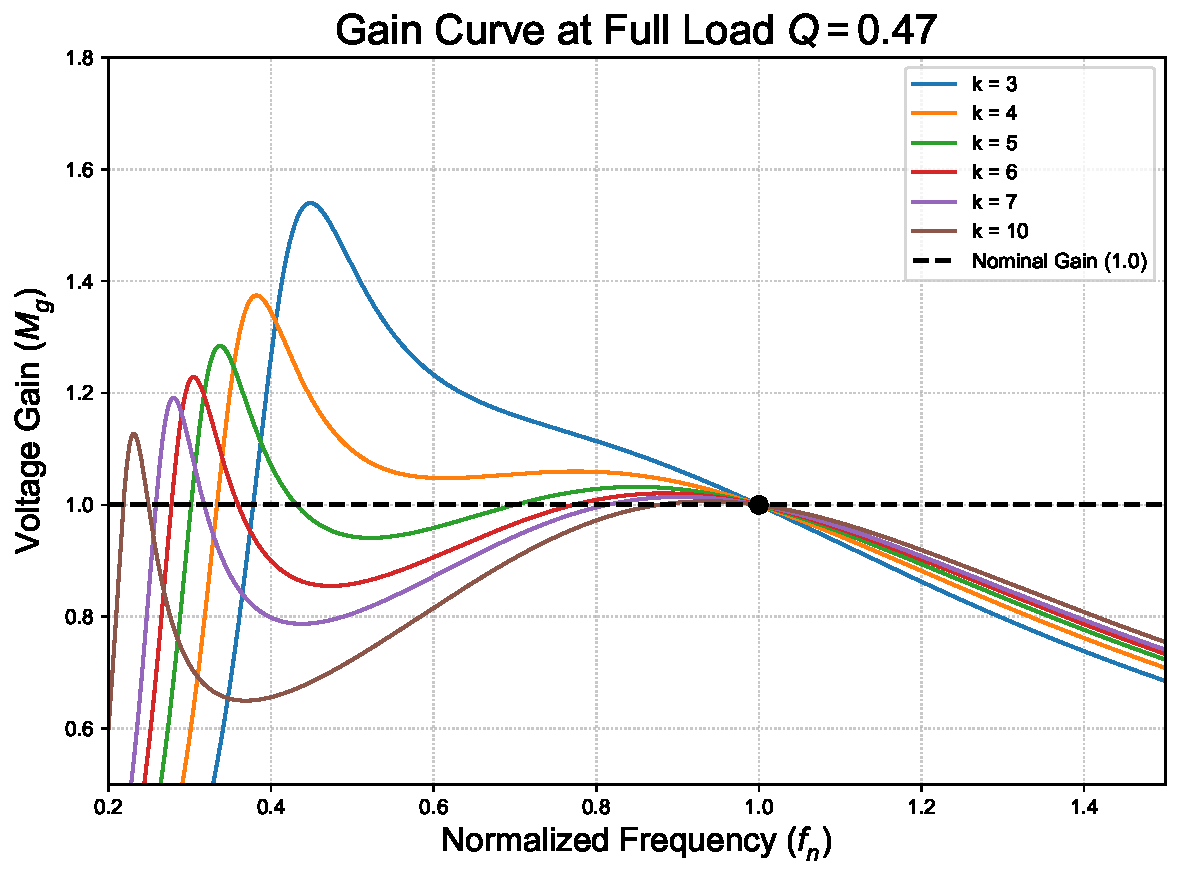
\includegraphics[width=0.5\columnwidth]{figures_chapter2/k_sweep_full_load.pdf} \label{fig:gainMax}
    }
     \subfloat[]{
        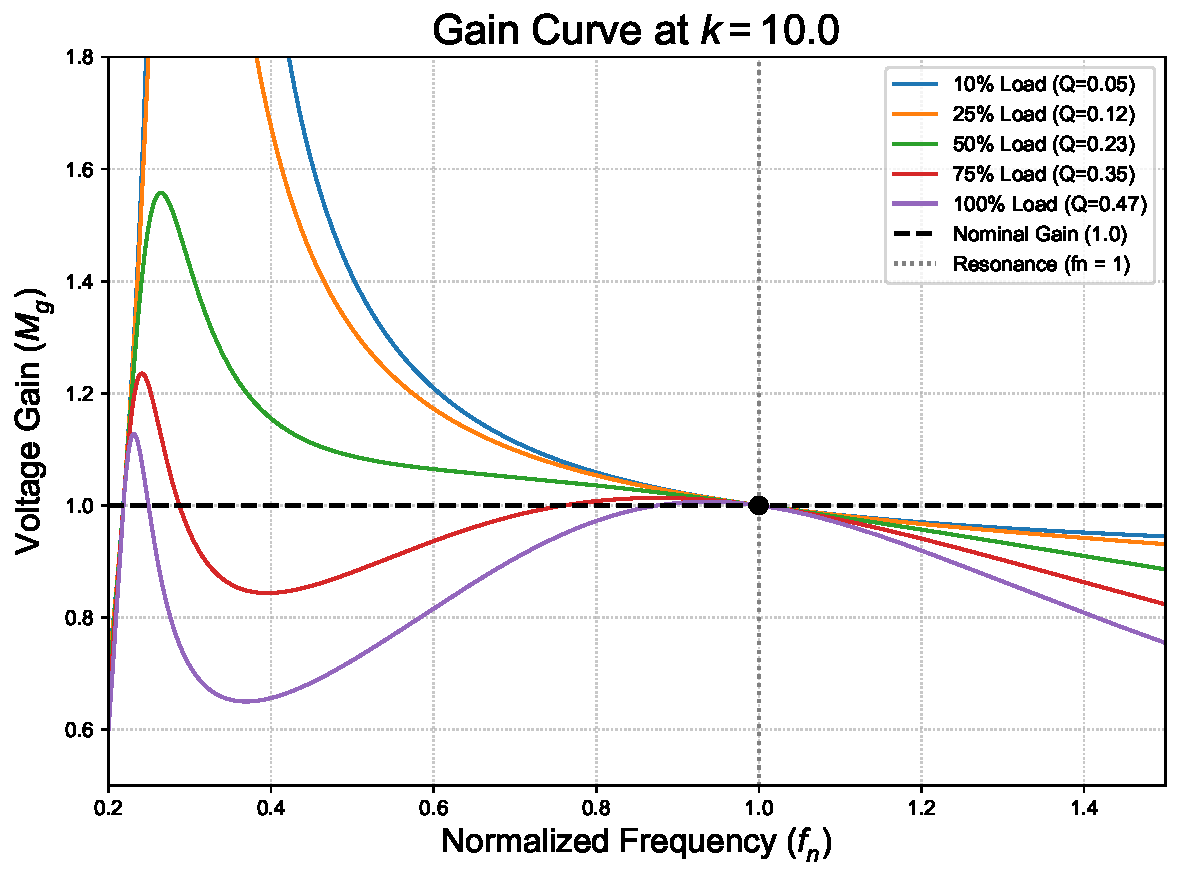
\includegraphics[width=0.5\columnwidth]{figures_chapter2/load_sweep_k10.pdf} \label{fig:gainAll}
    }
\caption{Gain curves of the CLLC at the operating specifications: (a) at max load, or max $Q$, and (b) at $k=10$.}
\end{figure}

\pagebreak
A few simulation waveforms are shown in the Appendix: \nameref{app:simulation}, confirming ZVS operation at 100 kW and 1 kW with the chosen parameters. Moreover, the following specifications are decided for the CLLC Converter, as shown in Table \ref{tab:1kW}.

\begin{table}[h!]
\centering
\caption{Established Converter Specifications for the Small-scale Study}
\label{tab:1kW}
\begin{tabular}{cccc}
\hline
\textbf{Parameter} & \textbf{Symbol} & \textbf{Value} \\
\hline \hline
Input Voltage & $V_{\mathrm{in}}$ & 100 V \\ 
Output Voltage & $V_{\mathrm{out}}$ & 100 V   \\
Switching Frequency & $f_{\mathrm{sw}}$ & 28.5 kHz \\ 
Output Power & $P_\mathrm{O}$ & 1 kW \\
Output Current & $I_\mathrm{O}$ & 10 A \\
\hline
Resonant Frequency & $f_{\mathrm{r}}$ & 30 kHz \\ 
Magnetizing Inductance & $L_\mathrm{m}$ & 200 $\upmu$H   \\
Leakage Inductance & $L_\mathrm{r1}\, L_\mathrm{r2}$ & 20.0 $\upmu$H \\ 
Resonant Capacitance & $C_\mathrm{r1}\, C_\mathrm{r2}$ & 1.4 $\upmu$F \\
Dead Time & $t_\mathrm{d}$ & 200 ns \\
\hline
\end{tabular}
\end{table}







\chapter{Transformer Design for Enhanced Thermal Management} \label{Chapter 3}
The volumetric power density of high-frequency resonant converters is fundamentally constrained by the thermal limits of the magnetic components. In high-power applications, the transformer is subjected to substantial high-frequency copper and core losses. This chapter details the fundamental design principles and analytical models employed to propose and size the proposed transformer without compromising its electromagnetic performance.

\section{Proposed Transformer Design}
In high-power-density CLLC resonant converters, managing the thermal stresses caused by high-frequency core and winding losses is a critical design constraint. As introduced in Section \ref{sec:cooling}, conventional solutions have a high dependence on active cooling systems to manage these thermal loads. This solution proposes to improve intrinsic thermal extraction from the heat-generating elements, which comprise the windings and the ferrite core, to the external ambient environment. With this solution, the dependence on active cooling methods has a potential to be reduced. 

Therefore, the proposed transformer is fundamentally engineered to improve this heat conduction by maximizing the core window utilization, and minimizing the internal-to-external thermal resistance. To facilitate this, a planar structure utilizing a low-loss Mn-Zn ferrite EE-core is proposed. 

Within this planar structure, the winding configuration is the primary determining factor for heat flow. There are two main configurations for rectangular windings in transformers. Conventionally, planar transformers typically utilize edgewise windings, where the rectangular conductor is wound on its narrow edge, along the vertical axis of the core. To address the inherent bottlenecks of the conventional winding structure, the proposed transformer utilizes solid rectangular windings arranged in a flatwise orientation. This entails that the winding is wound on its broad, flat side, resembling a radial stack propagating from the center.

The proposed structure utilizing a flatwise-wound configuration is shown in Figure \ref{fig:flatwise_3D_trans}. The cross-section of this design is shown in Figure \ref{fig:flatwise_2D_trans}. To ensure optimal thermal contact and maximize heat extraction toward the widest cooling area, a soft, silicon-based thermal-interface material (TIM) is sandwiched directly between the copper windings and the ferrite core interface.

\begin{figure}[h!]
    \centering
    \subfloat[]{
        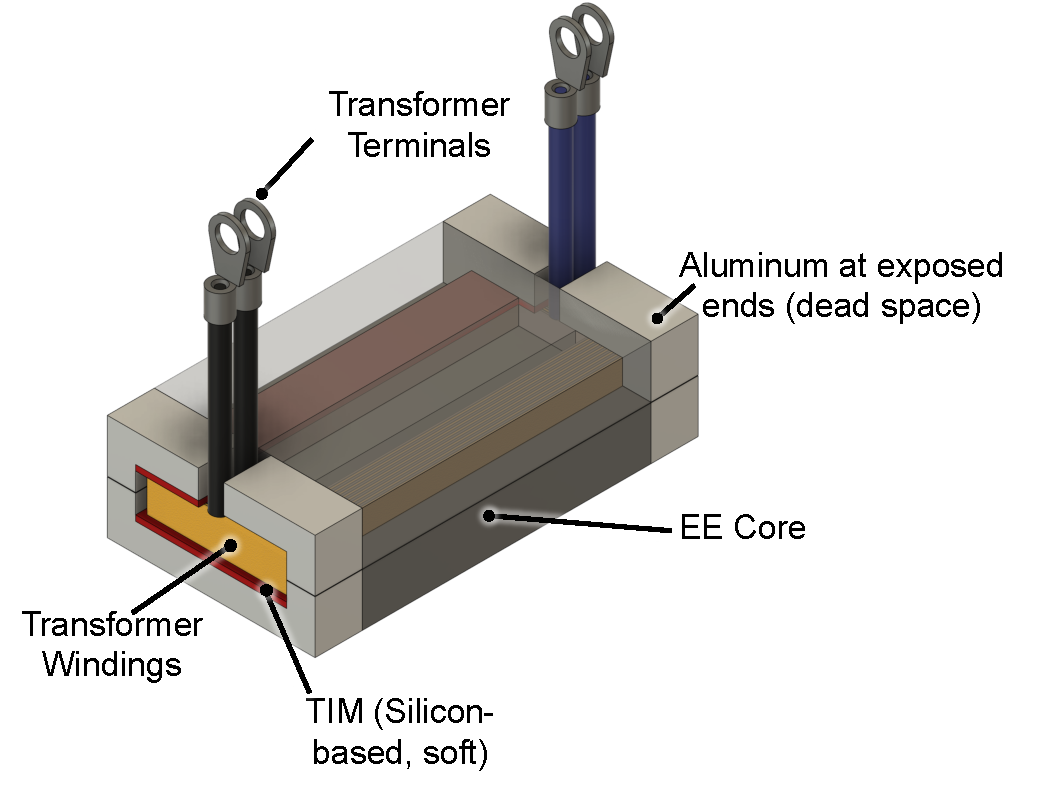
\includegraphics[width=0.5\columnwidth]{figures_chapter3/flatwise_3D.pdf}%
        \label{fig:flatwise_3D_trans}
    }
    \subfloat[]{
        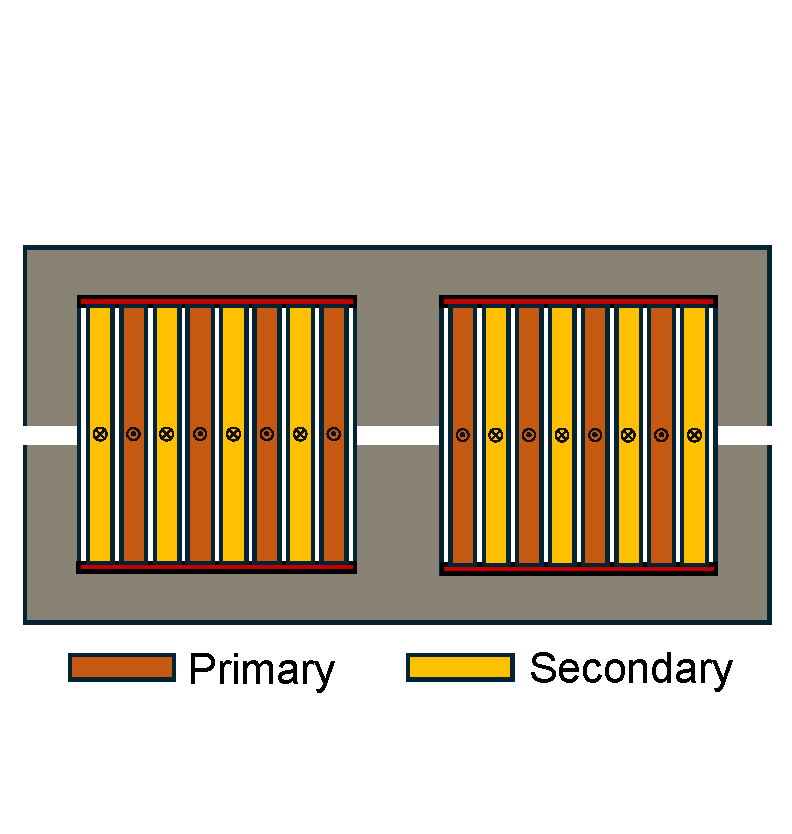
\includegraphics[width=0.3\columnwidth]{figures_chapter3/flatwise_cross.pdf}
        \label{fig:flatwise_2D_trans}
    }
    \caption{Representative model of an flatwise-wound transformer: (a) mockup of the transformer, with the top half of the EE core transparent, and (b) cross-sectional view of the transformer.}
    \label{fig:flatwise_design}
\end{figure}

In the subsequent chapters, this proposed flatwise structure will be rigorously compared against its conventional counterpart through both 3D FEA simulations and empirical hardware testing. The counterpart transformer employs an identical core and TIM structure, but utilizes a traditional edgewise-wound configuration, as shown in Figure \ref{fig:edgewise_3D_trans} and Figure \ref{fig:edgewise_2D_trans} respectively.

\begin{figure}[h!]
    \centering
    \subfloat[]{
        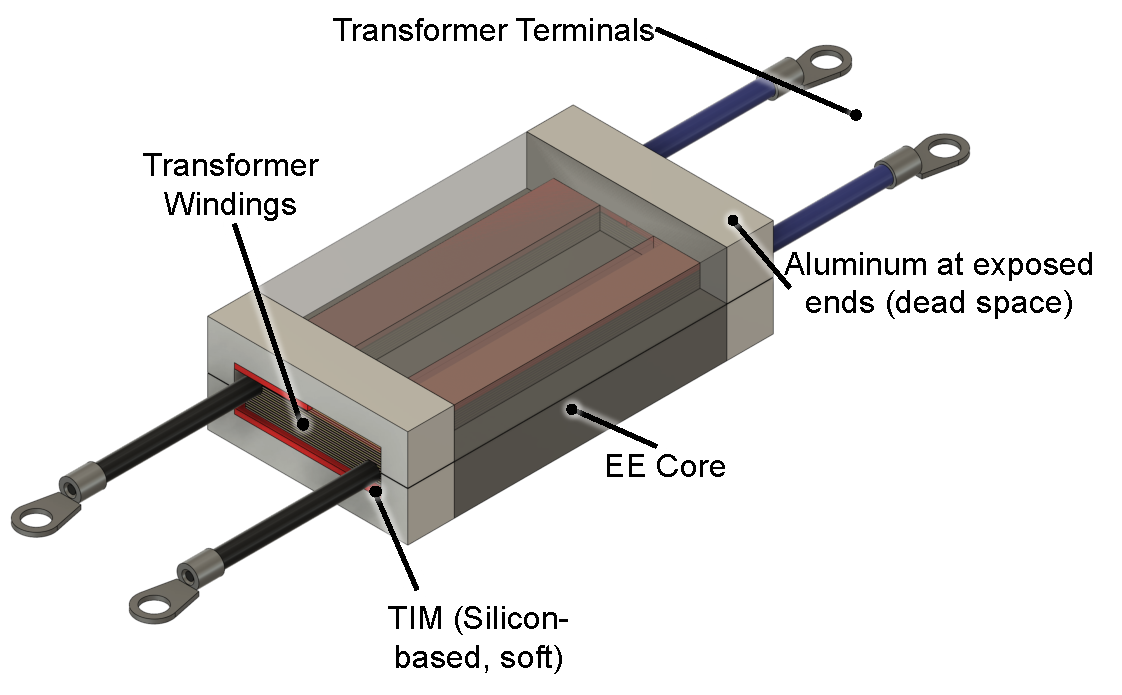
\includegraphics[width=0.5\columnwidth]{figures_chapter3/edgewise_3D.pdf}%
        \label{fig:edgewise_3D_trans}
    }
    \subfloat[]{
        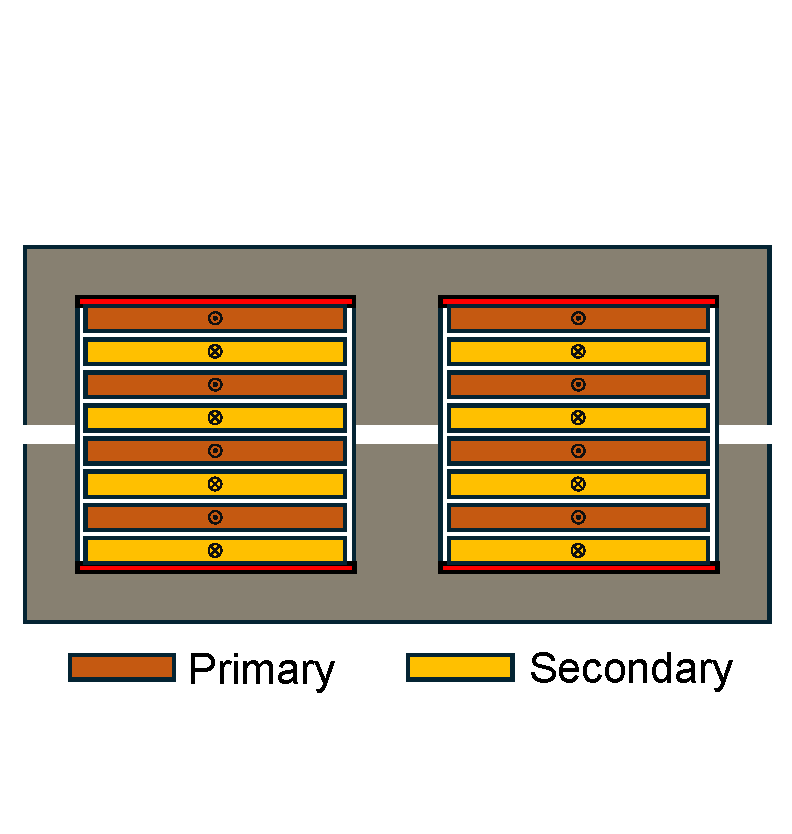
\includegraphics[width=0.3\columnwidth]{figures_chapter3/edgewise_cross.pdf}
        \label{fig:edgewise_2D_trans}
    }
    \caption{Representative model of an edgewise-wound transformer: (a) mockup of the transformer, with the top half of the EE core transparent, and (b) cross-sectional view of the transformer.}
    \label{fig:edgewise_design}
\end{figure}

\subsection{Heat Dissipation Mechanism}\label{section:heat_dissipation}

This section details the mechanism of heat extraction from the windings to the environment depending on the configuration. The design presented regardless of the winding configuration operates on the following principle. The primary thermal dissipation path through the windings is augmented by two supplementary mechanisms, as illustrated in Figure \ref{fig:heatdissipation}. First, the high fill factor enables heat to conduct directly from the copper through a thermal interface material (TIM) into the ferrite core, which functions as a heat spreader. Second, the exposed winding overhangs occupy the volume outside the EE-core, referred to as 'dead space'. This volume is leveraged by attaching aluminum blocks to the top and bottom surfaces of the exposed windings, creating an additional direct path for heat extraction. The heat flow from the lower winding section into the cooling block under external cooling conditions is also illustrated. The substantial surface area of this planar structure facilitates efficient heat transfer to external systems, such as liquid cold plates, which is essential for high-power density applications.

\begin{figure}[h!]
    \centering
    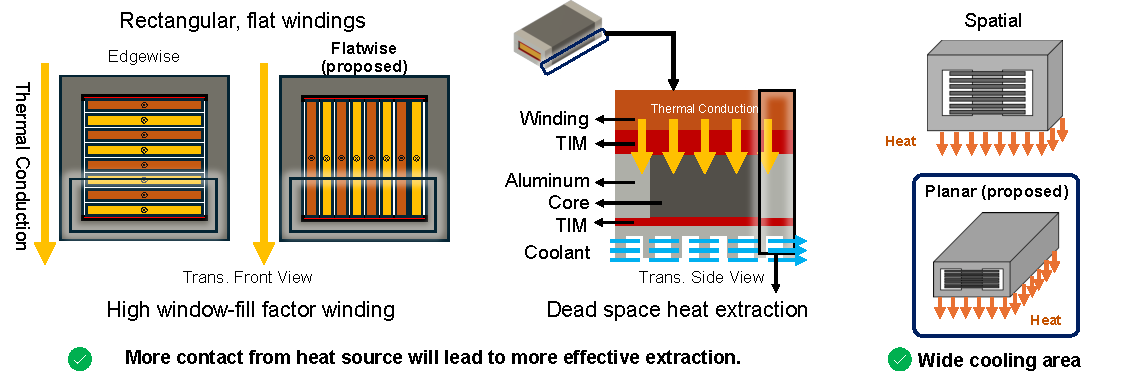
\includegraphics[width=\columnwidth]{figures_chapter3/heatdissipation.pdf}
    \caption{Heat conduction paths for the transformers, with a primary heat transfer path through the windings and supplementary path through an aluminum block in the ‘dead space’, with an external cooling system. The wide surface area for cooling aids in heat dissipation from the transformer.}
    \label{fig:heatdissipation}
\end{figure}

The advantage of the proposed structure compared to its conventional counterpart will be explained once the thermal models are established for each configuration.

\subsection{Winding Configuration}

While optimizing the thermal dissipation path is critical, minimizing internal heat generation is equally important. In high-frequency transformers, winding interleaving is a proven strategy to reduce the peak magnetomotive force (MMF), thereby mitigating AC copper losses driven by skin and proximity effects. To determine the optimal balance of performance and manufacturability for the proposed transformer, this study evaluates three winding configurations: non-interleaved, Primary-Secondary-Secondary-Primary (PSSP) \cite{ref21}, and fully interleaved. A comparison of their extracted parasitic parameters is presented in Table \ref{tab:parasitics}, while their physical implementation is illustrated in Figure~\ref{fig:implementation}.

\begin{table}[h]
    \caption{Comparison of Parasitic Parameters}
    \centering
    
        \begin{tabular}{cccccc}
            \hline
            \textbf{Parameter} & \textbf{Symbol} & \textbf{Non-Inter.} & \textbf{PSSP Inter.} & \textbf{Full Inter.} & \textbf{Unit} \\
            \hline \hline
            AC Res. & $R_{\mathrm{AC}}$ & 40.05 & 21.45 & 21.56 & m$\Omega$ \\
            Interwinding Cap. & $C_{\mathrm{ps}}$ & 0.15 & 0.96 & 1.72 & nF \\
            Leakage Ind. & $L_{\mathrm{lk}}$ & 2.63 & 0.07 & 0.04 & $\upmu$H \\
            \hline
        \end{tabular}%
    
    \label{tab:parasitics}
\end{table}

\begin{figure}[h]
    \centering
    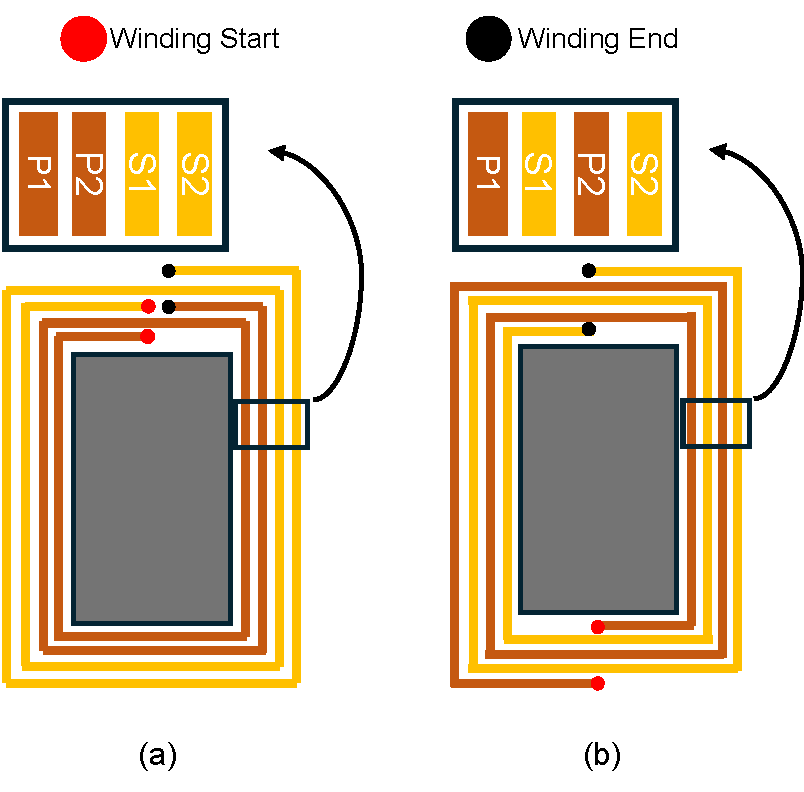
\includegraphics[width=0.5\columnwidth]{figures_chapter3/interleaving implementation.pdf}
    \caption{Schematic representation of the implementation of the interleaving strategies discussed (top view): (a) no interleaving, and (b) full interleaving. Four turns are shown for easy interpretation.}
    \label{fig:implementation}
    
\end{figure}

The selection of the winding arrangement requires balancing leakage inductance, parasitic capacitance, and manufacturability. The fully interleaved model demonstrates the lowest leakage inductance (0.04 $\upmu\text{H}$), a substantial improvement over the non-interleaved baseline (2.63 $\upmu\text{H}$). While this configuration increases the interwinding capacitance to 1.72 nF due to the larger effective overlap area, circuit simulations verify that this capacitance level does not hinder the ZVS operation of the CLLC converter. Conversely, while the non-interleaved model offers minimal capacitance (0.15 $\text{nF}$), the associated high leakage inductance and AC resistance result in prohibitive losses for this high-power density application.

The PSSP configuration presents an intermediate trade-off, offering reduced AC resistance (21.45 $\text{m}\Omega$) with moderate capacitance. However, PSSP interleaving introduces significant manufacturability constraints. Moreover, as this was examined in a discrete turn case, then once the winding becomes continuous, it would not be implementable.

Therefore, the fully interleaved configuration is selected. It provides the optimal balance by minimizing AC losses and maintaining circuit stability.

\section{Transformer Modelling}

\subsection{Geometric Model}
To establish a lot of the terms to be used in the subsequent sections, a geometric model is first defined. To simplify the analysis, the windings will be treated as discrete layers per turn. A parametric geometric model is created for the flatwise-wound transformer based on the winding dimensions ($w_{\mathrm{wire}}$, $h_{\mathrm{wire}}$), number of turns ($N_{\mathrm{p}}$), and the inter-winding distance ($d_{\mathrm{inter}}$), allotted for isolation. An air gap $l_\mathrm{g}$ is also included. The TIM thickness ($d_{\mathrm{TIM}}$) and core clearances ($d_{\mathrm{clear}}$) are also considered in determining the final core dimensions. A similar model is also derived for the edgewise-wound transformer. The models for the edgewise-wound and flatwise-wound transformers are shown in Figure~\ref{fig:edgewise_parameter} and \ref{fig:flatwise_parameter} respectively. This flow of modelling is inspired by \cite{bahmani2016design}.

\begin{figure}[h!]
    \centering
    \subfloat[]{
        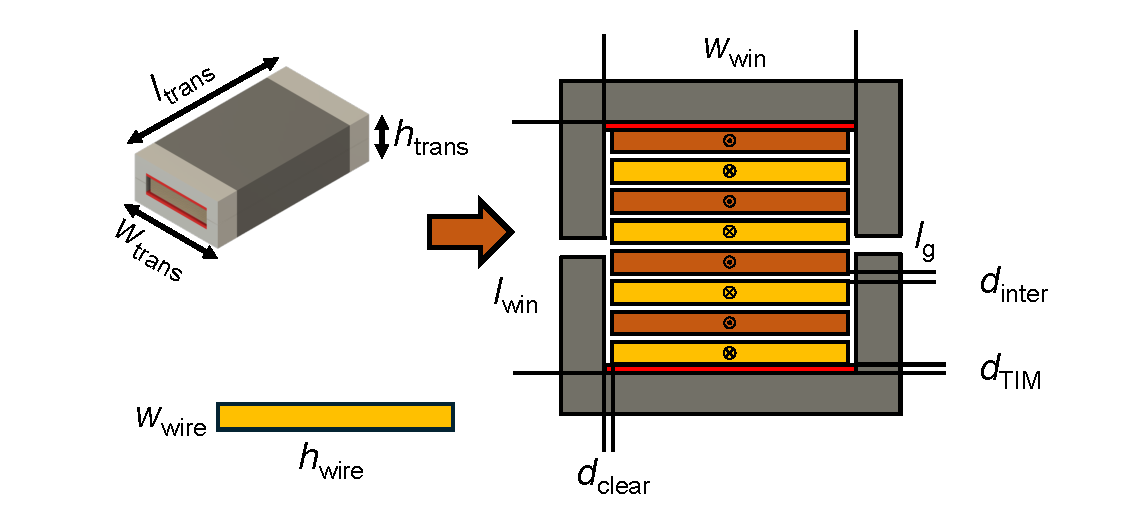
\includegraphics[width=0.85\columnwidth]{figures_chapter3/edgewise_parameter.pdf}%
        \label{fig:edgewise_parameter}
    }

    \subfloat[]{
        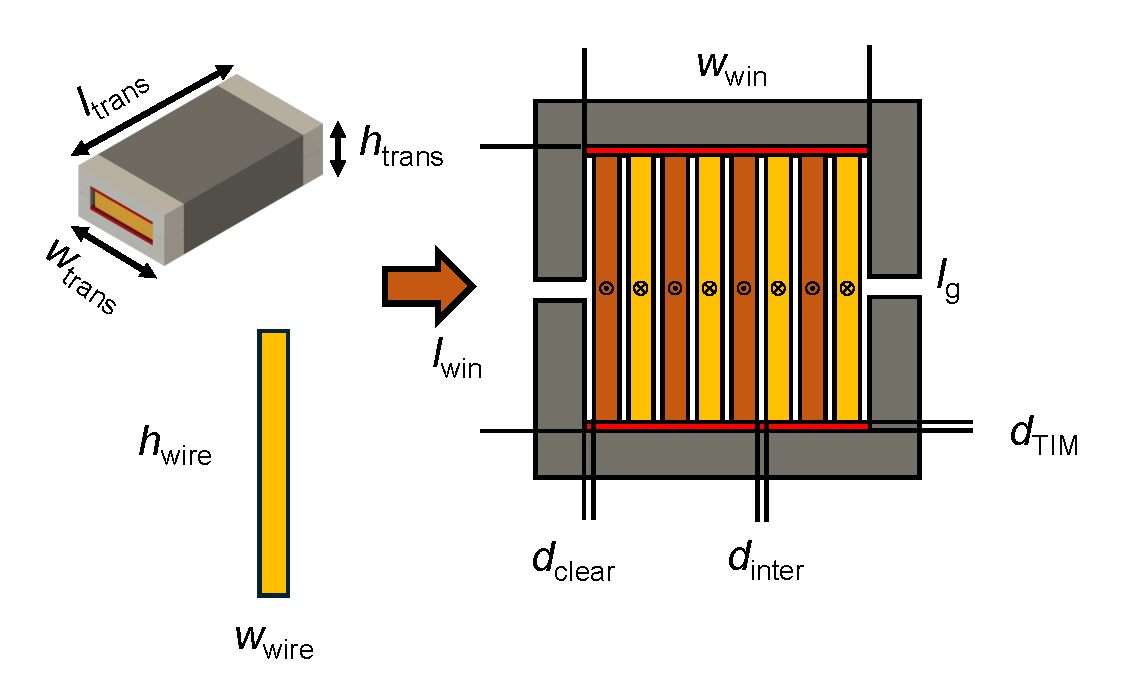
\includegraphics[width=0.8\columnwidth]{figures_chapter3/flatwise_parameter.pdf}
        \label{fig:flatwise_parameter}
    }
    \caption{Parametric model of an (a) edgewise-wound transformer (conventional) and (b) flatwise-wound transformer (proposed).}
    \label{fig:parameteric models}
\end{figure}

The core window dimensions are important to obtain other geometric parameters of the transformer. The window height $h_{\mathrm{win}}$ and width $w_{\mathrm{win}}$ can be obtained with the following as shown in Eq.~\ref{eq:hwin} and Eq.~\ref{eq:wwin} respectively for the flatwise-wound transformer. 
\begin{align}
    h_{\mathrm{win}} &= h_{\mathrm{wire}} + 2 d_{\mathrm{TIM}} \label{eq:hwin} \\
    w_{\mathrm{win}} &= 2N_{\mathrm{p}} w_{\mathrm{wire}} + (2N_{\mathrm{p}} - 1) d_{\mathrm{inter}} + 2 d_{\mathrm{clear}} \label{eq:wwin}
\end{align}

For the conventional counterpart, the equations look similar, with Eq. ~\ref{eq:hwinedge} and Eq. ~\ref{eq:wwinedge} representing the window height and width respectively. 
\begin{align}
    h_{\mathrm{win}} &= 2N_{\mathrm{p}} w_{\mathrm{wire}} + (2N_{\mathrm{p}} - 1) d_{\mathrm{inter}} + 2 d_{\mathrm{TIM}} \label{eq:hwinedge}\\
    w_{\mathrm{win}} &= h_{\mathrm{wire}} + 2 d_{\mathrm{clear}} \label{eq:wwinedge}
\end{align}
A few more quantities can be obtained after looking at the transformer from the top. From Figure \ref{fig:core_top}, $l_\mathrm{core}$ and $w_\mathrm{core}$ represent the length and width of the center leg respectively. As per commercial standard, the width of the outer leg is half of $w_\mathrm{core}$. 

\begin{figure}[h!]
    \centering
    \subfloat[]{
        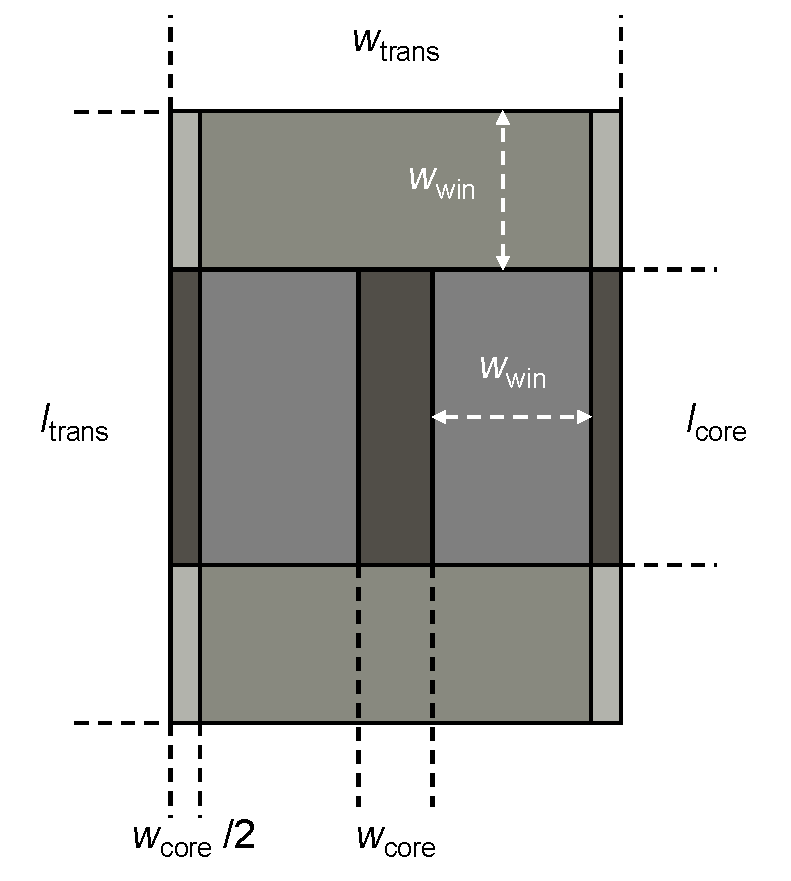
\includegraphics[width=0.5\columnwidth]{figures_chapter3/core_top.pdf}%
        \label{fig:core_top}
    }

    \subfloat[]{
        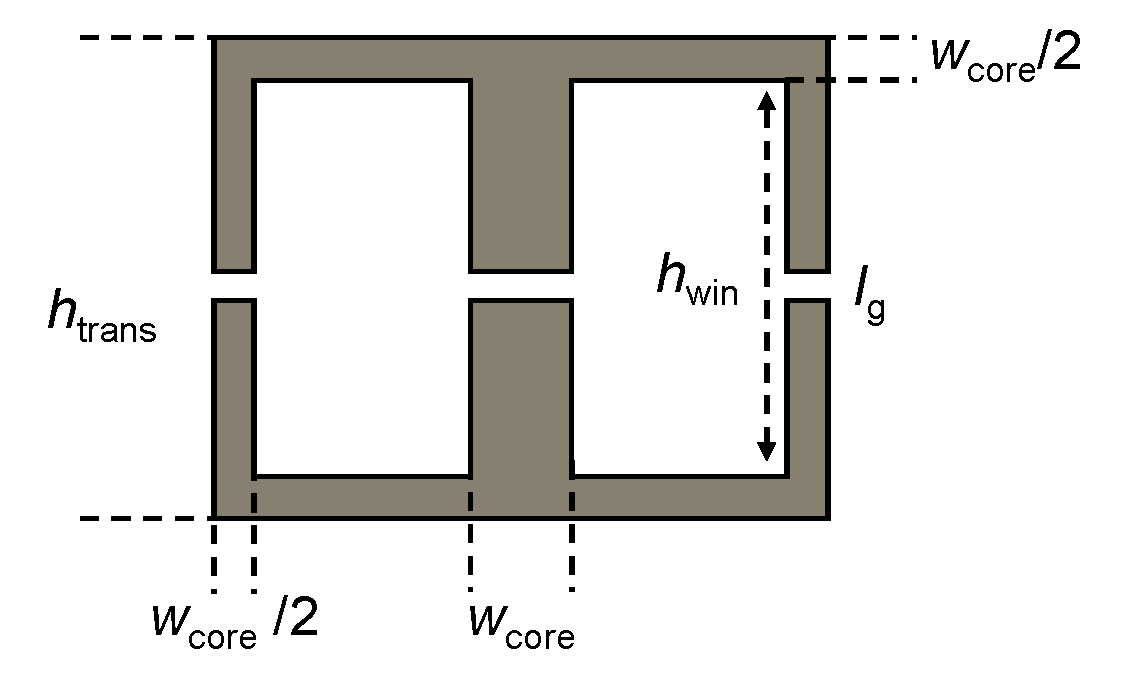
\includegraphics[width=0.5\columnwidth]{figures_chapter3/core_front.pdf}
        \label{fig:core_front}
    }
    \caption{(a) Top view and (b) Front view of the transformer geometric model.}
    \label{fig:parameteric models core}
\end{figure}

The transformer dimensions are obtained by using Eq.~\ref{eq:ltrans} --~\ref{eq:htrans}. Moreover, the aluminum block for dead space has a length of $w_{\mathrm{win}}$ regardless of the winding configuration. The TIM is applied throughout the top and bottom of the core window with width $w_{\mathrm{win}}$, ensuring maximum contact between the windings and the heat spreader. The box dimensions are represented in Figure \ref{fig:parameteric models}.
\begin{align}
    l_{\mathrm{trans}} &= l_{\mathrm{core}} + 2w_{\mathrm{win}}  \label{eq:ltrans}\\
    w_{\mathrm{trans}} &= w_{\mathrm{core}} + 2 w_{\mathrm{win}} + 2 \cdot \frac{w_\mathrm{core}}{2} \label{eq:wtrans}\\
    h_{\mathrm{trans}} &= 2 \cdot \frac{w_\mathrm{core}}{2} + h_{\mathrm{win}}\label{eq:htrans} 
\end{align}


Lastly, the mean turn length (MTL) of each of the configurations can be denoted by Eq. ~\ref{eq:MTL}. A simpler analogy to denote this is that the mean turn length is the length of the turn halfway through the core window. 
\begin{align}
    \mathrm{MTL} &= 2l_{\mathrm{core}} + 2w_{\mathrm{core}} + 8w_{\mathrm{win}} \label{eq:MTL} 
\end{align}

\subsection{Thermal Modeling}
To evaluate the fundamental heat dissipation mechanisms of the conventional edgewise and proposed flatwise winding configurations, analytical 1D Thermal Networks are constructed, as they are highly effective and widely adopted for planar magnetics \cite{ref13}, \cite{escribano2006new}, \cite{lewaiter2001thermal}, \cite{vanderlinde1991design}, \cite{chen2002volumetric}. Because the primary external cooling boundaries (the TIM and core) are located at the top and bottom of the winding window, the dominant conductive heat flux is strictly unidirectional (vertical). Therefore, lateral (side-to-side) heat transfer across the winding window can be mathematically neglected, allowing a simplified 1D thermal resistance network to accurately capture the primary heat extraction path.

In a thermal model, each loss source is modeled as a discrete current source. For a transformer, this includes the winding loss and core loss. The winding loss is separated per turn, denoted as $P_{\mathrm{Np1}}\, , P_{\mathrm{Ns1}}\, , \dots \, , P_{\mathrm{Npn}}\, , P_{\mathrm{Nsn}}$ while the core loss is defined as $P_{\mathrm{core}}$. Moreover, to extract heat away from the transformer towards the ambient $T_\mathrm{amb}$, radiation $R_\mathrm{rad}$ and convection $R_\mathrm{conv}$ are taken into account and are placed towards the end of the network, at both sides. Additional thermal resistances are added depending on the cooling method. But for the purposes of explaining the concept, these are not added yet.

A comparative representation of the heat flow towards the cooling boundaries must be analyzed through the fundamental equation for conductive thermal resistance:
\begin{equation}
R_{\mathrm{th}} = \frac{d}{k \cdot A}
\label{eq:Rth}
\end{equation}
where $d$ is the conduction path length, $k$ is the thermal conductivity of the material, and $A$ is the cross-sectional heat transfer area. 

It is important to note that the models that will be presented here are for the purpose of explaining the proposed concept. 3D FEA will be used to provide accurate thermal mapping and visualization. 

A common design concern when comparing the flatwise and edgewise structures is the apparently restricted heat extraction area of the flatwise configuration. In the flatwise winding, the surface area of each individual turn directly facing the primary cooling boundary (the TIM and core) is indeed limited to the narrow, thin edge of the rectangular conductor. Conversely, the conventional edgewise configuration places the wide, broad side of the top and bottom turns directly in contact with the cooling plane. 
To calculate the true physical heat transfer area, the 2D cross-sectional contact width must be multiplied by the orthogonal depth of the winding trace going into the core window $l_{\mathrm{depth}}$. In this analysis, a rectangular section of the core is considered, with width $w_\mathrm{win}$ and length $l_\mathrm{depth}$. Furthermore, because the flatwise turns are positioned side-by-side, the total available window width $w_{\mathrm{win}}$ must be shared between the copper edges and the inter-turn dielectric insulation $d_{\mathrm{inter}}$. The total physical copper contact area for the flatwise configuration is defined as:
\begin{equation}
A_{\mathrm{contact, flat}} = l_{\mathrm{depth}} \cdot \sum_{i=1}^{N} w_{\mathrm{wire}, i} = l_{\mathrm{depth}} \cdot \left( w_{\mathrm{win}} - \sum_{j=1}^{N-1} d_{\mathrm{inter}, j} - 2 d_\mathrm{clear}\right)
\end{equation}

Conversely, the conventional edgewise configuration places the broad side of the top and bottom turns directly in contact with the cooling plane. The total copper contact area is therefore:
\begin{equation}
A_{\mathrm{contact, edge}} = l_{\mathrm{depth}} \cdot h_{\mathrm{wire}} = l_{\mathrm{depth}} \cdot \left(w_\mathrm{win} - 2d_\mathrm{clear}\right)
\end{equation}

Therefore, the flatwise configuration mathematically presents a smaller physical copper contact area to the external TIM ($A_{\mathrm{contact, flat}} < A_{\mathrm{contact, edge}}$) due to the spatial penalty of the vertical insulation strips.

The critical divergence that overcomes this area reduction lies in the network topology and the extreme discrepancy between the thermal conductivities of copper ($k_{\mathrm{Cu}} \approx 400 \text{ W/(m}\cdot\text{K)}$) and dielectric insulation materials ($k_{\mathrm{ins}} \approx 0.1 \text{ to } 0.2 \text{ W/(m}\cdot\text{K)}$).

\subsubsection{Edgewise-wound Transformer Thermal Model}
In the conventional edgewise configuration, the windings are stacked vertically, creating a series thermal path. Because the turns are stacked on top of one another, the heat generated in the innermost turns (e.g., Turn $N/2$) must conduct vertically through multiple layers of copper and, crucially, multiple layers of inter-turn insulation to reach the external cooling boundary.  Here, $N = 2N_\mathrm{p}$. A simple illustration of the heat flow from the windings to the core is shown in Figure \ref{fig:edgewise_heat}. 

\begin{figure}[h!]
    \centering
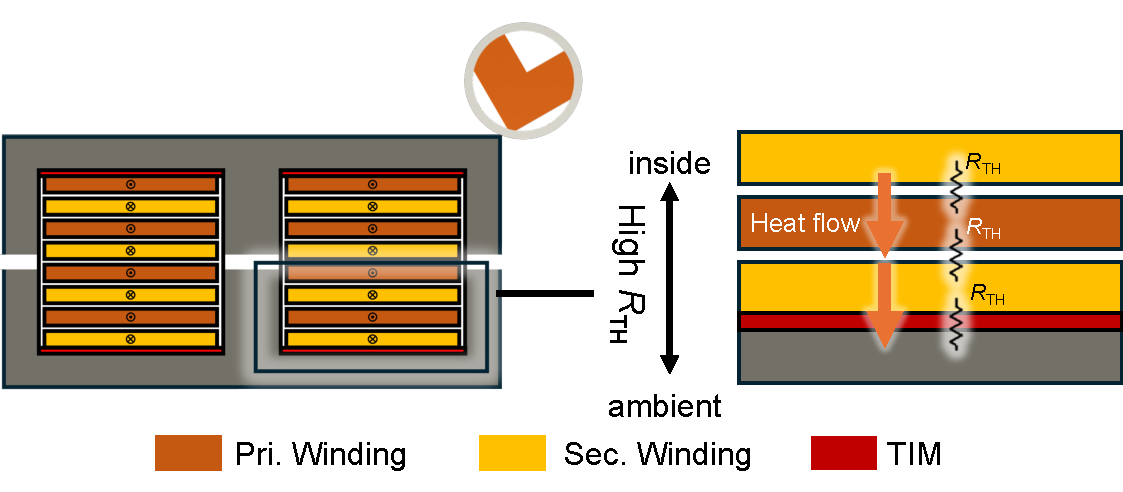
\includegraphics[width=0.8\columnwidth]{figures_chapter3/edgewise_heat.pdf} 
\caption{Simple representation of the edgewise-wound (conventional) transformer, with the cross-sectional area of the transformer. The heat flow direction
is also illustrated through a close-up.} \label{fig:edgewise_heat}
\end{figure}

Even though the heat transfer area $A_{\mathrm{contact, edge}}$ is large, it is severely obstructed by the series addition of multiple insulation thermal resistances ($R_{\mathrm{ins}}$). Because $k_{\mathrm{ins}}$ is approximately 2000 to 4000 times lower than $k_{\mathrm{Cu}}$, even a sub-millimeter layer of dielectric insulation acts as an immense thermal wall.

The thermal model for the edgewise-wound transformer is shown in Figure \ref{fig:edgewise_thermalmodel}. The total internal thermal resistance of the edgewise stack from the center to the cooling boundary is expressed as shown in Equation \ref{eq:edgewise_rth}. 
\begin{equation}
R_{\mathrm{th, edgewise}_\mathrm{total}} = \frac{N}{2} \left( \frac{w_{\mathrm{wire}}}{k_{\mathrm{Cu}} \cdot h_{\mathrm{wire}} \cdot l_\mathrm{depth}} + \frac{d_{\mathrm{inter}}}{k_{\mathrm{ins}} \cdot h_{\mathrm{wire}} \cdot l_\mathrm{depth}} \right) \label{eq:edgewise_rth}
\end{equation}
As $N$ scales, the summation of the high-resistance insulation terms dominates the network, trapping heat in the center turns. 
\begin{figure}[h!]
    \centering
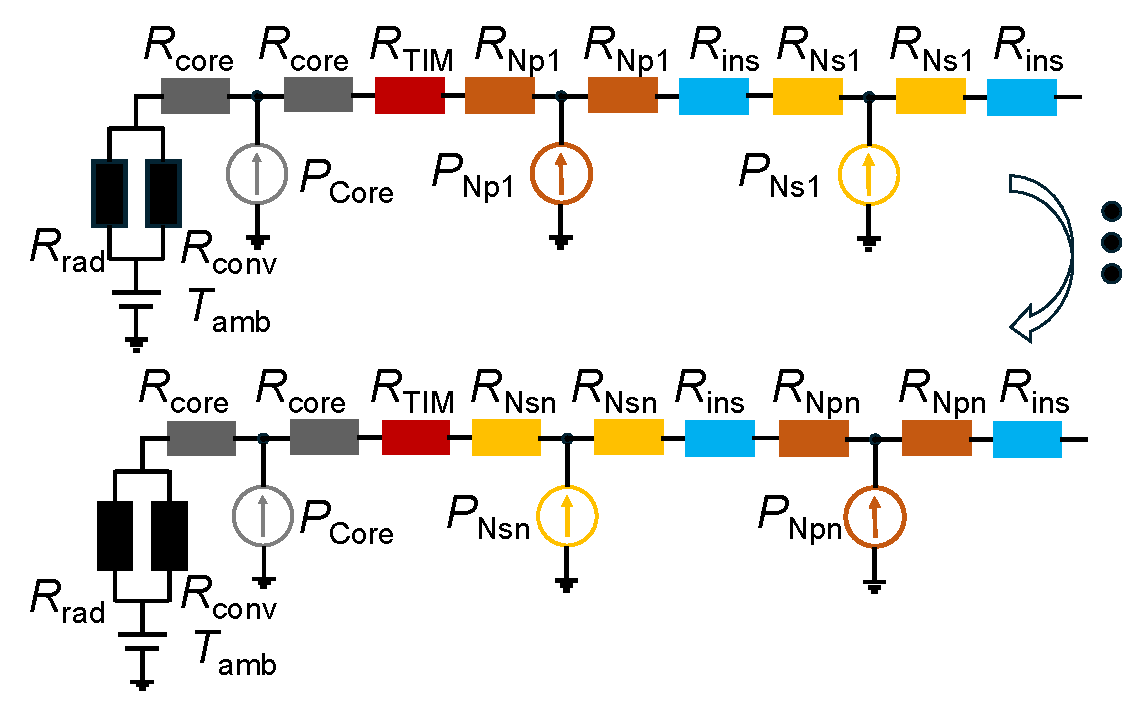
\includegraphics[width=0.8\columnwidth]{figures_chapter3/edgewise_thermalpath.pdf}
\caption{Thermal model for the edgewise-wound (conventional) transformer.}\label{fig:edgewise_thermalmodel}
\end{figure}
\subsubsection{Flatwise-wound Transformer Thermal Model}
In the proposed flatwise configuration, the turns are wound flat and propagate radially outward. This configuration transforms the series thermal trap into a highly efficient parallel thermal path. A simple illustration of the heat flow from the windings to the core is shown in Figure \ref{fig:flatwise_heat}. 
\begin{figure}
    \centering
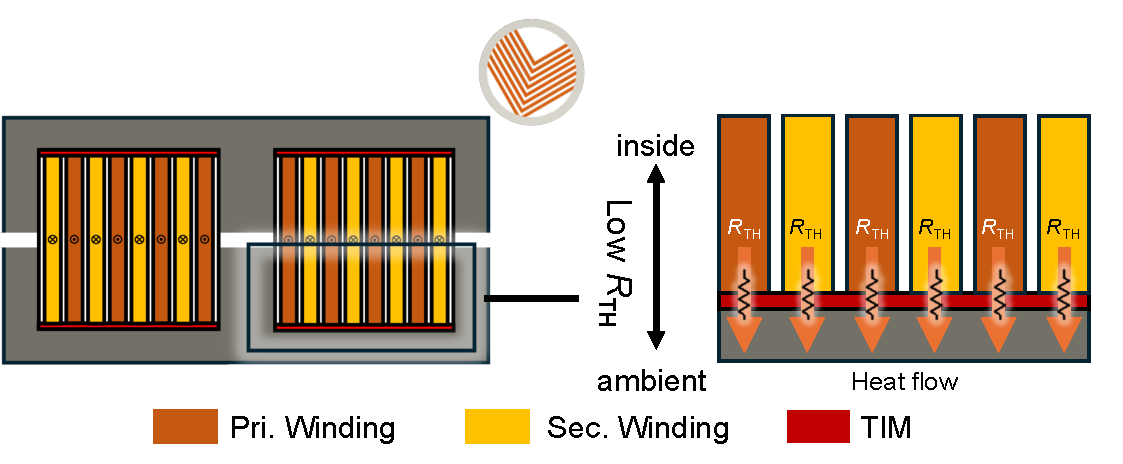
\includegraphics[width=0.8\columnwidth]{figures_chapter3/flatwise_heat.pdf}
\caption{Simple representation of the flatwise-wound (proposed) transformer, with the cross-sectional area of the transformer. The heat flow direction
is also illustrated through a close-up.}\label{fig:flatwise_heat}
\end{figure}

Because the turns are positioned side-by-side, every single individual turn maintains direct, independent contact with the top and bottom TIM and cooling boundaries via its narrow edge. To escape, the heat generated inside any given turn only needs to travel vertically through its own solid copper body to its exposed edge. It does not cross a single inter-turn dielectric insulation barrier ($d_{\mathrm{inter}}$) in series. The parallel thermal resistance of the flatwise winding is defined as shown in Eq. \ref{eq:flatwise_rth}. Here, $N = 2N_\mathrm{p}$.
\begin{equation}
R_{\mathrm{th, flatwise_\mathrm{total}}} = \frac{1}{\left(N\cdot  \frac{h_{\mathrm{wire}}/2}{k_{\mathrm{Cu}} \cdot w_{\mathrm{wire}}\cdot l_\mathrm{depth}} \right)^{-1}}\label{eq:flatwise_rth}
\end{equation}

Although the physical contact area per turn is restricted to $h_{\mathrm{wire}}$, the heat conduction path is entirely within solid copper. Because copper is an exceptionally efficient thermal conductor, the low resistance of the continuous copper path easily compensates for the reduced contact area. 

\begin{figure}
    \centering
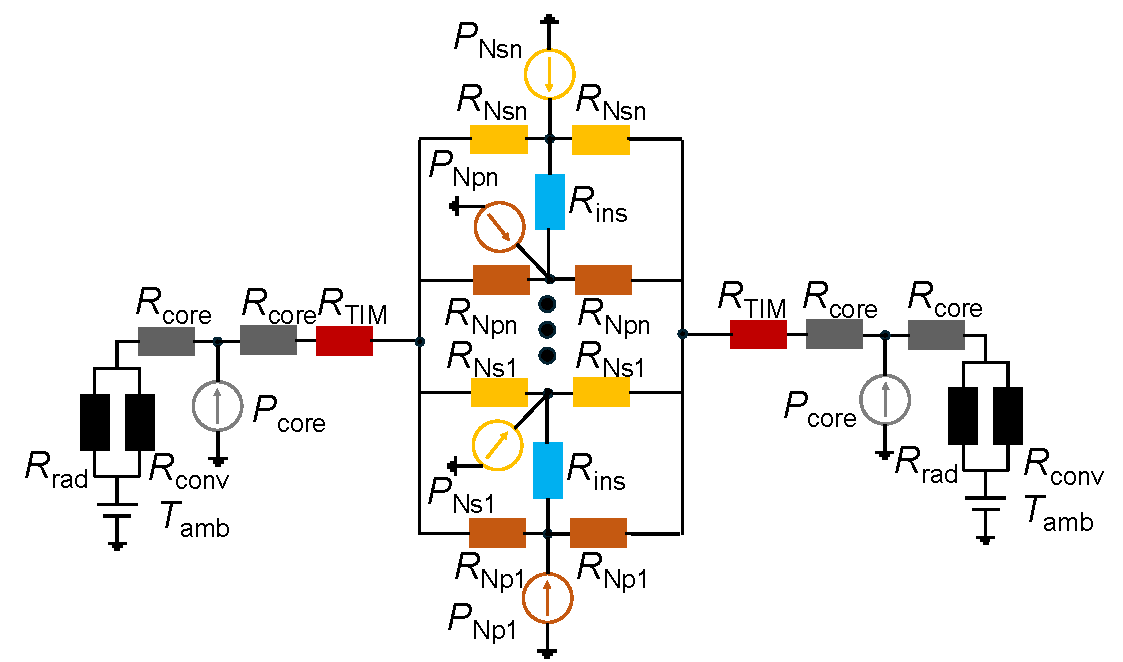
\includegraphics[width=0.8\columnwidth]{figures_chapter3/flatwise_thermalpath.pdf}
\caption{Thermal model for the edgewise-wound (conventional) transformer.}\label{fig:flatwise_thermalmodel}
\end{figure}

 By utilizing a low-resistance parallel copper path in the flatwise design, the proposed transformer fundamentally eliminates internal thermal barriers, enabling highly efficient, simultaneous uniform heat extraction directly from the windings to the core window. It is expected that a more uniform distribution of temperature will be seen throughout the transformer.


%The efficiency of this internal heat dissipation can be explicitly examined through the use of thermal models. A thermal model translates the physical geometry into an equivalent network of thermal resistances to evaluate conductive heat transfer from the internal layers to the ambient environment. For this study, 1D-Thermal Models are constructed. With planar magnetics, the dominant heat extraction path remains to be the surfaces.

%While 3D Finite Element Analysis (FEA) provides comprehensive spatial mapping, analytical 1D lumped-parameter thermal networks are highly effective and widely adopted for planar magnetics \cite{ref15, bahmani2016}. As established in recent planar thermal reviews, the inherent high surface-area-to-volume ratio of flat magnetic structures results in a dominant conductive heat flux that is strictly orthogonal. Therefore, transverse and longitudinal heat transfer can be mathematically neglected, allowing a 1D thermal resistance model to accurately capture the primary path of least thermal resistance.

%In a thermal model, each loss source is modeled as a discrete current source. For a transformer, this includes the winding loss and core loss. The winding loss is separated per turn, denoted as $N_p1, ..., N_pn$. Moreover, to extract heat away from the transformer, radiation and convection are taken into account and are placed towards the end of the network, at both sides. Additional thermal resistances are added depending on the cooling method. But for the purposes of explaining the concept, these are not added yet. Additionally, the thermal resistance of an element $R_{\mathrm{th}}$ is defined as follows:


%The conventional edgewise configuration creates a high-resistance series thermal path that tends to trap heat in the central layers. The corresponding thermal model of the edgewise-wound transformer is shown in Figure xx, derived using the principles from [13].

%In contrast, the proposed flatwise configuration creates a parallel thermal path from winding to core, enabling direct and simultaneous heat extraction from each individual turn. This results in a significantly lower overall internal thermal resistance compared to the conventional counterpart. The thermal model of the flatwise-wound transformer is shown in Figure xx. This then entails a more even heat distribution and lower peak temperature.

%From here on out, a simplified transformer model will be used to examine and easily optimize the dimensions. Each turn will be treated as a discrete turn, stacked from top to bottom for the edgewise-wound transformer, and from center to outward for the flatwise wound transformer, both wound at the center leg.

%In contrast, the proposed flatwise configuration creates a parallel thermal path from winding to core, enabling direct and simultaneous heat extraction from each individual turn. This results in a significantly lower overall internal thermal resistance compared to the conventional counterpart. The thermal model of the flatwise-wound transformer is shown in Figure \ref{fig:fig3b}. This then entails a more even heat distribution and lower peak temperature.

%In the subsequent sections, a simplified transformer model will be used to examine and easily optimize the dimensions. 

\subsection{Isolation Distance}
As mentioned in Section \ref{sec:challenge}, isolation is required to be able to cater to higher voltage applications. It is not yet a current focus of the study. However, ensuring that the transformer is able to cater to basic capabilities is important. It is set as a basic constraint for the transformer, as it essentially affects the overall geometry depending on the number of turns. Moreover, because the windings are rectangular, then the electric field distribution between each primary and secondary turn can be approximated to be the same as that of a parallel-plate capacitor \cite{bahmani2016design}.

Because the windings are rectangular, the windings can be approximated as plate capacitors. Therefore, the minimum isolation distance $d_{\mathrm{inter, min}}$ can be defined as in Eq. \ref{eq:iso, min}.
\begin{align}
d_\mathrm{inter, min} = \frac{V_\mathrm{ins}}{k_\mathrm{saf}E_\mathrm{ins}}\label{eq:iso, min}
\end{align}
\noindent where $V_\mathrm{ins}$ is the expected voltage requirement, and $E_\mathrm{ins}$ is the dielectric material breakdown strength. A safety factor $k_{\mathrm{saf}}$ is also included. 

For the minimum clearance between the windings and the core, $d_{\mathrm{clear, min}}$, it is assumed that the core will be grounded in higher power applications \cite{bahmani2016design}. Therefore, $d_{\mathrm{clear, min}}$ can be estimated with the operating voltage $V_{\mathrm{in}}$, as shown in Eq. \ref{eq:clear, min}. The same equation can be used to estimate the minimum thickness of the TIM, $d_\mathrm{TIM, min}$.
\begin{align}
d_\mathrm{clear, min} = d_\mathrm{TIM, min} = \frac{V_\mathrm{in}}{k_\mathrm{saf}E_\mathrm{ins}}\label{eq:clear, min}
\end{align}

The distance is calculated first and then further confirmed in FEM if it suits the criteria. This is explained further in the next chapter, section \ref{sec:breakdown}.

\subsection{Magnetic Circuit}
A baseline magnetic circuit model is established to evaluate the magnetization properties of the transformer, as indicated in Figure \ref{fig:mag}. The outer leg and core leg magnetic reluctances are denoted as $\mathcal{R}_\mathrm{mo}$ and $\mathcal{R}_\mathrm{mc}$ respectively. The gap reluctances in the outer and center legs are denoted as $\mathcal{R}_\mathrm{go}$ and $\mathcal{R}_\mathrm{gc}$ respectively. 

For this analytical derivation, the transformer is initially assumed to have ideal magnetic coupling, as further strengthened by the full interleaving strategy employed in this transformer. This is assumed to decouple the resonant tank design from the thermal evaluation of the winding structure. Instead, discrete resonant inductors are employed for the resonant tank of the converter.  The secondary side is deactivated (open-circuited) to isolate the primary magnetizing flux, which yields the fundamental expression for the primary magnetizing inductance as shown in Eq. \ref{eq:Lm}:
\begin{equation}
L_\mathrm{m} = \frac{N_\mathrm{p}^2}{\mathcal{R}_{\mathrm{m, eq}}}\label{eq:Lm}
\end{equation}
where $N_p$ is the primary number of turns and $\mathcal{R}_\mathrm{m, eq}$ is the total equivalent reluctance of the magnetic path.

\begin{figure}
    \centering
    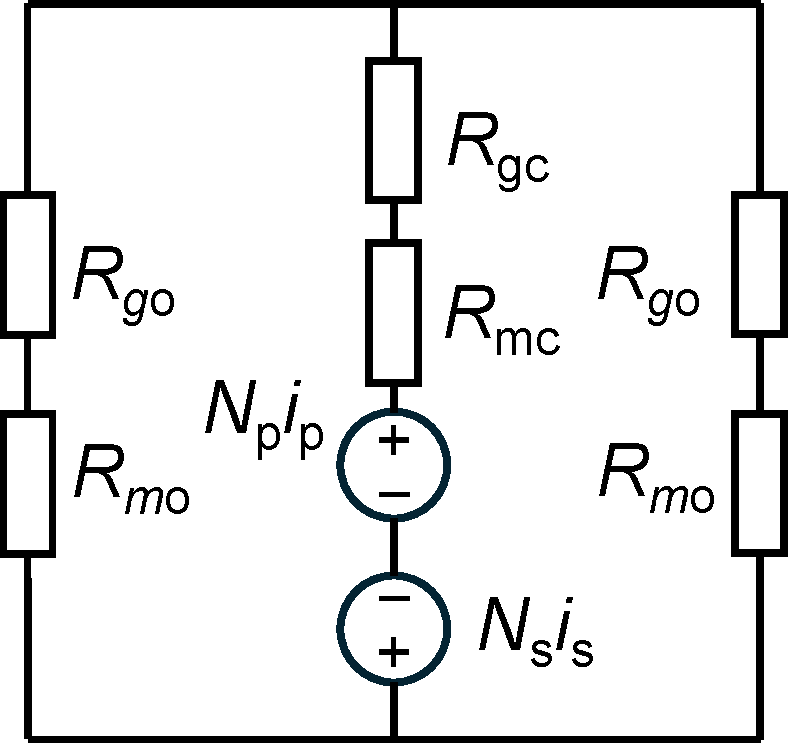
\includegraphics[width=0.35\columnwidth]{figures_chapter3/magnetic_circuit.pdf} 
    
    \caption{Magnetic circuit considered for the proposed transformer in this study.} \label{fig:mag}
\end{figure}

An air gap ($l_g$) is deliberately introduced into the core legs to increase the total reluctance, thereby preventing magnetic saturation under high current excitation and also at operating temperature. Since the transformer is expected to have a wide cross-sectional area, and it is important to obtain an accurate magnetizing inductance for the ZVS operation of the converter, the fringing effect is taken into account when obtaining the cross-sectional area $A_\mathrm{core}$ for the transformer. The method described in \cite{muhlethaler2011novel} is utilized to fine-tune $A_\mathrm{core}$.

\subsection{Core Loss Model}
The improved Generalized Steinmetz Equation (iGSE) is used to obtain the core losses and is able to accommodate a variety of excitation waveforms for the transformer \cite{ref14}. The loss density of a transformer is given in Eq. \ref{eq:igse}, and is multiplied to the core volume to obtain the total core loss:
\begin{equation}
P_{\mathrm{v}} = \frac{1}{T} \int_{0}^{T} k_i \left| \frac{dB}{dt} \right|^\alpha (\Delta B)^{\beta-\alpha} \, dt
\label{eq:igse}
\end{equation}
\noindent with $k_i$ defined in Eq. \ref{eq:ki}:
\begin{equation}
k_i = \frac{k}{(2\pi)^{\alpha-1} \int_{0}^{2\pi} |\cos \theta|^\alpha 2^{\beta-\alpha} \, d\theta}
\label{eq:ki}
\end{equation}
\noindent where $B$ represents the flux density in the transformer during operation, $T$ is the switching period, and $k$, $\alpha$ and $\beta$ represent the Steinmetz parameters of the core material obtained from the datasheet.

For a CLLC, the $B_\mathrm{pk}$ and $\Delta B$ is defined in Eq. \ref{eq:Bpk} and \ref{eq:delB} respectively.
\begin{align}
B_{\mathrm{pk}} &= \frac{V_{\mathrm{pri, pk}} \cdot T_\mathrm{s}}{4 \cdot N_\mathrm{p} \cdot A_{\mathrm{core}}}\label{eq:Bpk}\\
\Delta B &= \frac{V_{\mathrm{pri, pk}} \cdot \frac{T_s}{2}}{N_\mathrm{p}\cdot A_{\mathrm{core}}} \label{eq:delB}
\end{align}
where $V_{\mathrm{pri, pk}}$ is the peak primary side voltage,  $T_\mathrm{s}$ is the switching period, $N_\mathrm{p}$ is the number of turns in the primary side, and $A_\mathrm{core}$ is the cross-sectional area of the transformer center leg.

\subsection{Winding Loss Model}
Dowell's model for rectangular windings with a high width ($h_{\mathrm{wire}}$ for the proposed transformer) to thickness ($w_{\mathrm{wire}}$ for the proposed transformer) ratio, is presented in Equation \ref{eq:dowell} \cite{ref15, ref16}. This equation determines the resistance factor $F_{\mathrm{R}}$ for a turn, defined as the ratio of AC resistance to DC resistance:
\begin{equation}
\begin{split}
F_{\mathrm{R}} = \frac{\xi}{2} \Bigg[ &\frac{\sinh \xi + \sin \xi}{\cosh \xi - \cos \xi} + (2m^2 - 1) \frac{\sinh \xi - \sin \xi}{\cosh \xi + \cos \xi} \Bigg]
\end{split}
\label{eq:dowell}
\end{equation}
\noindent where the first and second terms represent the effects due to the proximity and skin effects, respectively. Moreover, $\xi$ and $m$ represent the penetration ratio and $m$-factor respectively. The penetration ratio $\xi$ is defined as $\xi = w_{\mathrm{wire}}/\delta$ for the flatwise-wound transformer. The skin depth $\delta$  at the operating frequency is given by Eq. \ref{eq:skindepth}:
\begin{equation}
\delta = \sqrt{\frac{\rho}{\pi \mu_r \mu_0 f_\mathrm{s}}}
\label{eq:skindepth}
\end{equation}
\noindent where $\rho$ is the resistivity of the conductor material, which is copper for the windings, $\mu_r$ and $\mu_0$ are the relative permeabilities of the conductor and free space respectively, and $f_s$ is the switching frequency.

The $m$-factor represents the total magnetomotive force ($F$) at a certain turn, divided by its change compared to $F$ at the first turn, as described in Eq. \ref{eq:mfactor}:
\begin{equation}
m = \frac{F(h)}{F(h)-F(0)}
\label{eq:mfactor}
\end{equation}
\noindent For a fully-interleaved winding configuration, $m = 1$.
The winding loss is defined as Eq. \ref{eq:loss}:
\begin{equation}
P_{\mathrm{wind}} = I_{\mathrm{wind}}^2 R_{\mathrm{AC, total}}
\label{eq:loss}
\end{equation}

\noindent where $I_{\mathrm{wind}}$ is the rms value of the transformer winding current and $R_{\mathrm{AC, total}}$ is the total AC Resistance of all turns. For the circuit used in this study, it is approximated to be the input power $P_{\mathrm{in}}$ divided by the input voltage $V_{\mathrm{in}}$ because the transformer is designed on a 1:1 turns ratio.  

\section{Design Considerations}
\par The proposed transformer is designed for a 1kW bidirectional CLLC resonant converter, as had been described in Chapter 2. The detailed specifications are summarized in Table \ref{tab:specs}.
\begin{table}[h]
    \caption{CLLC Converter Specifications}
    \centering
        \begin{tabular}{cccc}
            \hline
            \textbf{Parameter} & \textbf{Symbol} & \textbf{Value} & \textbf{Unit} \\
            \hline \hline
            Input Voltage & $V_{\mathrm{in}}$ & 100 & V \\
            Switching Frequency & $f_{\mathrm{s}}$ & 28.5 & kHz \\
            Primary Side Current & $I_{\mathrm{p, rms}}$ & 10 & A \\
            Transformer Turns Ratio & $n$ & 1 : 1& - \\
            Output Power & $P_{\mathrm{O}}$ & 1 & kW \\
            \hline
        \end{tabular}%
    \label{tab:specs}
\end{table}

\subsection{Design Method}
The design flow for the proposed transformer is depicted in Figure~\ref{fig:design_flow}. Initially, the circuit parameters and constraints are determined. A geometric model is then selected to ensure the transformer aspect ratio falls within the feasible range of 0.25 $\sim$ 0.75. Analytical calculations are then performed to verify that the core and winding losses are balanced ($P_{\mathrm{core}}/P_{\mathrm{wind}} \approx \text{0.50} - \text{1.50}$). The values provided here for the loss balance are just estimates and should be further fine-tuned or explored. Once these conditions are met, the model undergoes thermal and electromagnetic simulation. Ultimately, the design is accepted only if it satisfies the thermal limit of less than 100$^\circ$C peak temperature and maintains ZVS capability.

\begin{figure}[htbp]
    \centerline{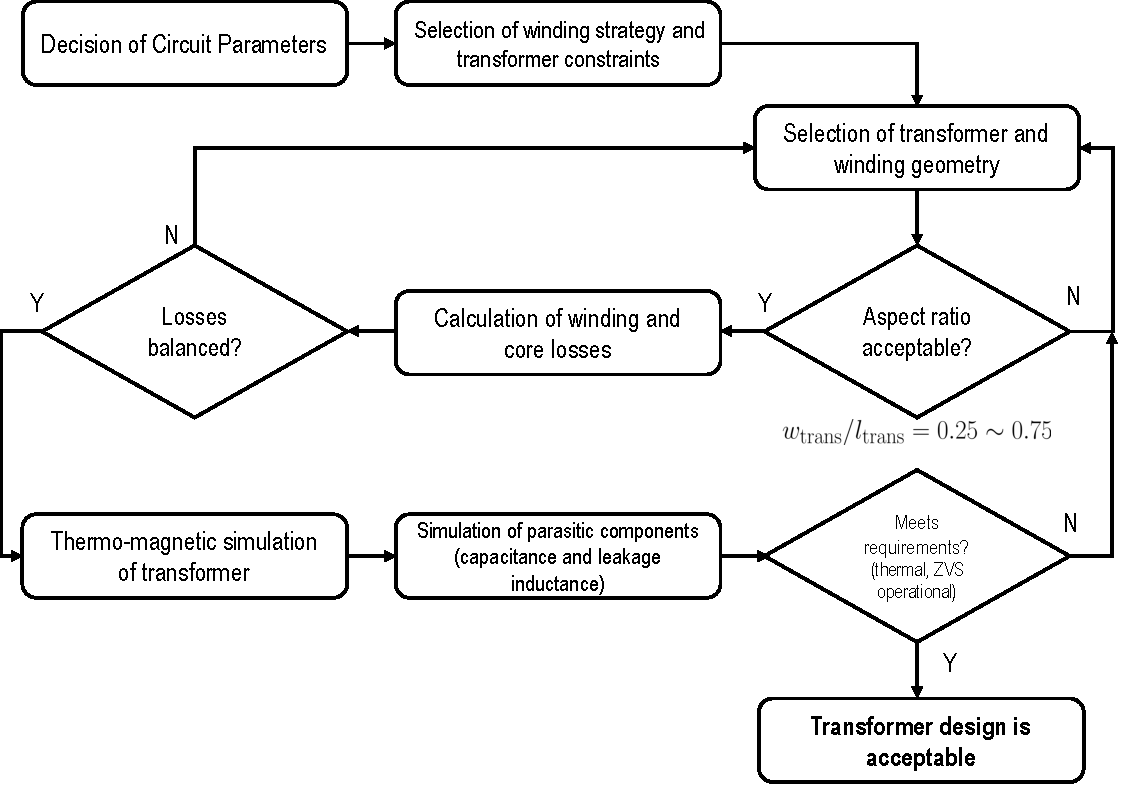
\includegraphics[width=\columnwidth]{figures_chapter3/designflow.pdf}}
    \caption{Design flow for the proposed transformer.}
    \label{fig:design_flow}
\end{figure}

\subsection{Magnetizing and Leakage Inductance}
As discussed in Section \ref{ref:FHA}, to ensure ZVS, the magnetizing inductance is constrained by Eq. \ref{eq:Lm_constraint}

\begin{equation}
L_m \le \frac{t_\mathrm{d}}{16 C_{\mathrm{oss}} f_{\mathrm{r}}}
\label{eq:Lm_constraint}
\end{equation}

\noindent where $t_{\mathrm{d}}$ is defined as the dead time, $C_{\mathrm{oss}}$ is the parasitic output capacitance of the switches, and $f_\mathrm{r}$ is the resonant frequency of the circuit.

\subsection{Number of Turns, Wire Thickness, and Inter-winding Distance}
\par As detailed in Section \ref{section:heat_dissipation}, maximizing the window fill factor is a primary design objective. Since a custom core is utilized to optimize the thermal path, careful selection of the winding geometry is crucial to minimize the overall transformer volume.

The number of turns, wire thickness, and inter-winding distance present trade-offs regarding the transformer volume and total losses. These trade-offs are examined to optimize the geometric parameters for high power density. For this comparison, the center leg width is fixed at 10 mm, the current density $J$ at 5 A/mm$^2$, and the magnetizing inductance $L_{\mathrm{m}}$ at 200 $\upmu$H. Moreover, $d_{\mathrm{TIM}}$ and $d_{\mathrm{clear}}$ are set to 1.00 mm each. The design is evaluated assuming a full interleaving configuration, as detailed in the subsequent subsection.

The interwinding distance $d_{\mathrm{inter}}$ is set to 0.10 mm, providing a safety factor of approximately two relative to the breakdown voltage of air (3 kV/mm) at the operating condition. Air was chosen as the insulation for this study, as the specifications do not entail high voltage yet. 

The design space is illustrated in Figure \ref{fig:trans_design}. The analysis reveals that increasing the number of turns significantly decreases the transformer volume, provided the wire width remains narrow. Conversely, increasing the wire width monotonically increases the volume; however, the rate of volume expansion depends on the turn count. Consequently, eight turns was identified as the optimal design point. Furthermore, the turn count, wire width, and spacing must be balanced to maintain a valid transformer aspect ratio.

The sensitivity of the volume and losses to the turn count emphasizes the necessity of minimizing $d_{\mathrm{inter}}$ until a safe breakdown threshold. Finally, $w_{\mathrm{wire}}$ is constrained to less than 2$\delta$ \cite{ref20}. This limit prevents the proximity effect from dominating the current distribution, which would otherwise induce excessive AC losses at the operating frequency. Based on the design space analysis, $w_\mathrm{wire}$ is selected as 0.30 mm. The resulting window area effectively becomes a square. The chosen design will be explained more in the next chapter.



An example of the loss calculation method analytically is provided in Appendix: \nameref{app:model} for the chosen design point $N_\mathrm{p} = 8$ and $w_\mathrm{wire} = 0.30$ mm.

\begin{figure}[t!]
    \centerline{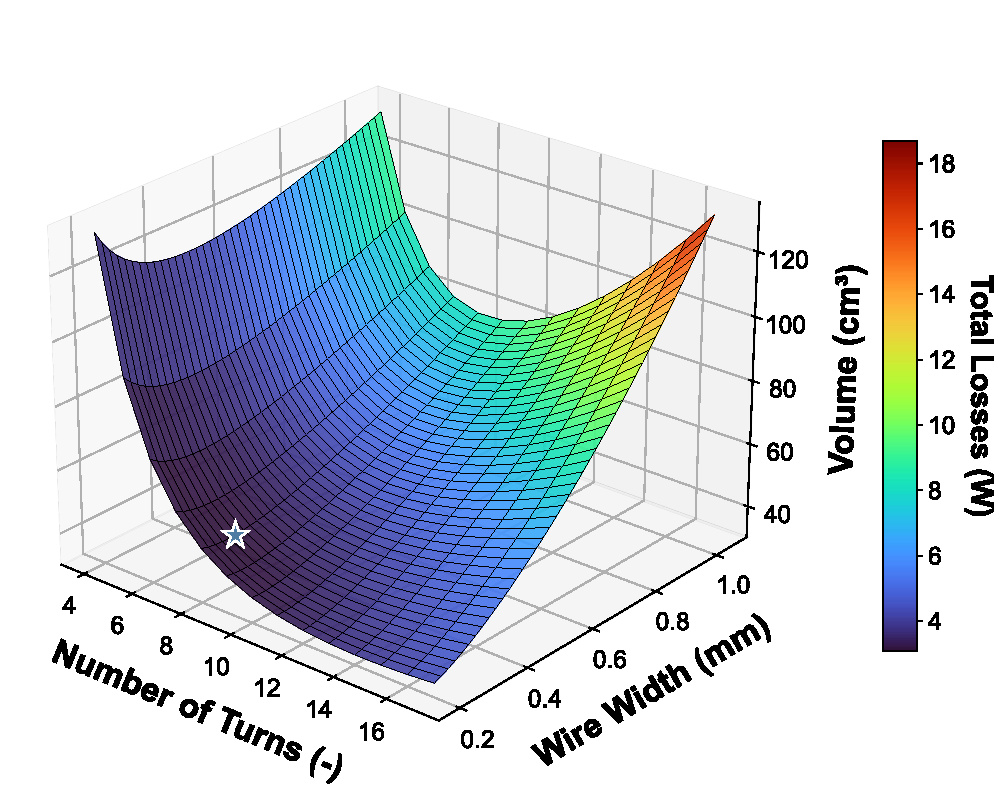
\includegraphics[width=0.8\columnwidth]{figures_chapter3/pareto.pdf}}
    \caption{Trade-off between number of turns and wire width for the flatwise-wound transformer. The selected design is marked as a star.}
    \label{fig:trans_design}
\end{figure}







\chapter{Simulation Analysis}
The proposed flatwise-wound transformer and its edgewise equivalent are simulated in Ansys Electronics using the Maxwell and Icepak solvers to check if the transformer design results in an electrically and thermally viable transformer. This chapter details the simulation conditions to carry out this evaluation. The results of the electromagnetic, electrostatic, and thermal simulations are described. Moreover, a geometric analysis is also performed to see the performance of the proposed winding under different profiles. 

It should also be emphasized that the primary objective of this simulation analysis is to compare the trends in temperature between the winding architectures. Due to the inherent mismatches between ideal simulation environments and practical hardware, particularly regarding complex high-frequency losses and exact thermal boundaries, these simulations serve strictly as a comparative evaluation tool.

\section{Simulation Conditions}
The proposed flatwise-wound transformer and its edgewise equivalent are simulated in Ansys Electronics. To ensure a fair comparison, key parameters were kept identical for both designs, especially the magnetizing inductance $L_{\mathrm{m}}$, number of turns $N_{\mathrm{p}}$, the window area $A_{\mathrm{win}}$, and the current density $J$. This equivalence ensures that the fundamental heat generation mechanisms in the windings and core are consistent, allowing for a direct comparison of the thermal dissipation capabilities of each structure. 

Using the design method presented in Section 3, the design parameters decided for the flatwise-wound transformer are detailed in Table \ref{tab:design_params}, and are simulated under the conditions in Table \ref{tab:specs}. An edgewise-wound transformer with identical wire geometry was also obtained. Since the window aspect ratio is approximately unity (square window), this constraint facilitates the use of a common core geometry for testing both winding configurations. 

\begin{table}[htbp]
    \caption{Transformer Design Parameters}
    \centering
    % Autofit to column width
    
        \begin{tabular}{ccccc}
            \hline
            \textbf{Parameter} & \textbf{Symbol} & \textbf{Flatwise} & \textbf{Edgewise} & \textbf{Unit} \\
            \hline \hline
            Magnetizing Inductance & $L_\mathrm{m}$ & 200.00 & 200.00 & $\upmu$H \\
            Air Gap & $l_\mathrm{g}$ & 0.10 & 0.10 & mm \\
            Number of turns & $N_\mathrm{p} : N_\mathrm{s}$ & 8 : 8 & 8 : 8 & - \\
            Core Permeability & $\upmu_\mathrm{r}$ & 3400 & 3400 & - \\
            Window Area & $A_{\mathrm{win}}$ & 76.56 & 76.56 & mm$^2$ \\
            Window Aspect Ratio & $l_{\mathrm{win}} / w_{\mathrm{win}}$ & $\sim 1.00$ & $\sim 1.00$ & - \\
            Current Density & $J$ & 5.00 & 5.00 & A/mm$^2$ \\
            \hline
        \end{tabular}%
    
    \label{tab:design_params}
\end{table}

More detailed setup conditions are presented in the Appendix: \nameref{app:ansys}.
\subsection{Electromagnetic Simulation Conditions}\label{electromagneticsim}
Electromagnetic simulation using Ansys Maxwell was performed to evaluate if the transformers will not saturate and if a correct magnetizing inductance was obtained. To approximate the square wave excitation from the CLLC converter while saving computational resources, a sinusoidal excitation with an equivalent RMS value was applied \cite{ref21}. To ensure that the transformer is simulated in its actual operating condition, providing both core and winding losses, the primary side is excited with a 100 V rms sinusoidal voltage, and the secondary side is excited with 10 A rms sinusoidal current in the opposite direction, representing the conditions at full load. The Eddy Current Solver was used for this set of simulations. The losses of each loss-generating element, which includes the aluminum, EE-core, and the copper winding, are coupled with the same model in the Icepak Environment to assume heat generation in the transformer is similar to its real operation. A simplified transformer model was used for the transformers as shown in Figure \ref{fig:sim_model_edgewise} and Figure \ref{fig:sim_model_flatwise} respectively.

\begin{figure}[h!]
    \centering
    \subfloat[]{
        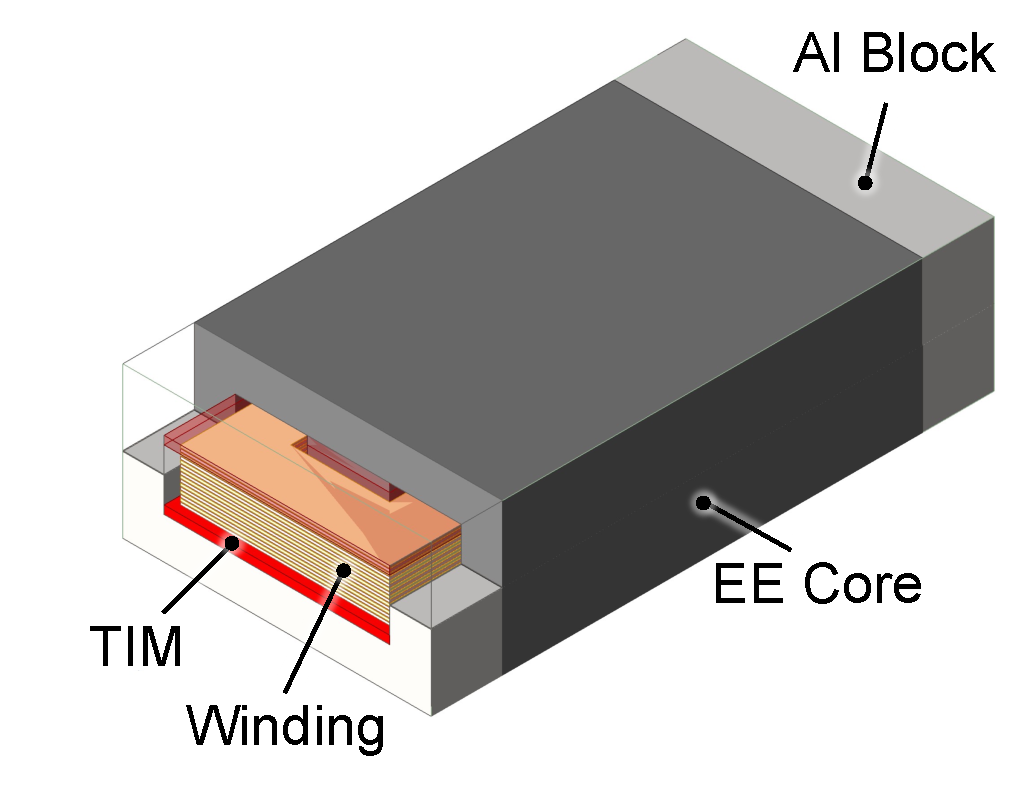
\includegraphics[width=0.5\columnwidth]{figures_chapter4/edgewise_simmodel.pdf}%
        \label{fig:sim_model_edgewise}
    }
    \subfloat[]{
        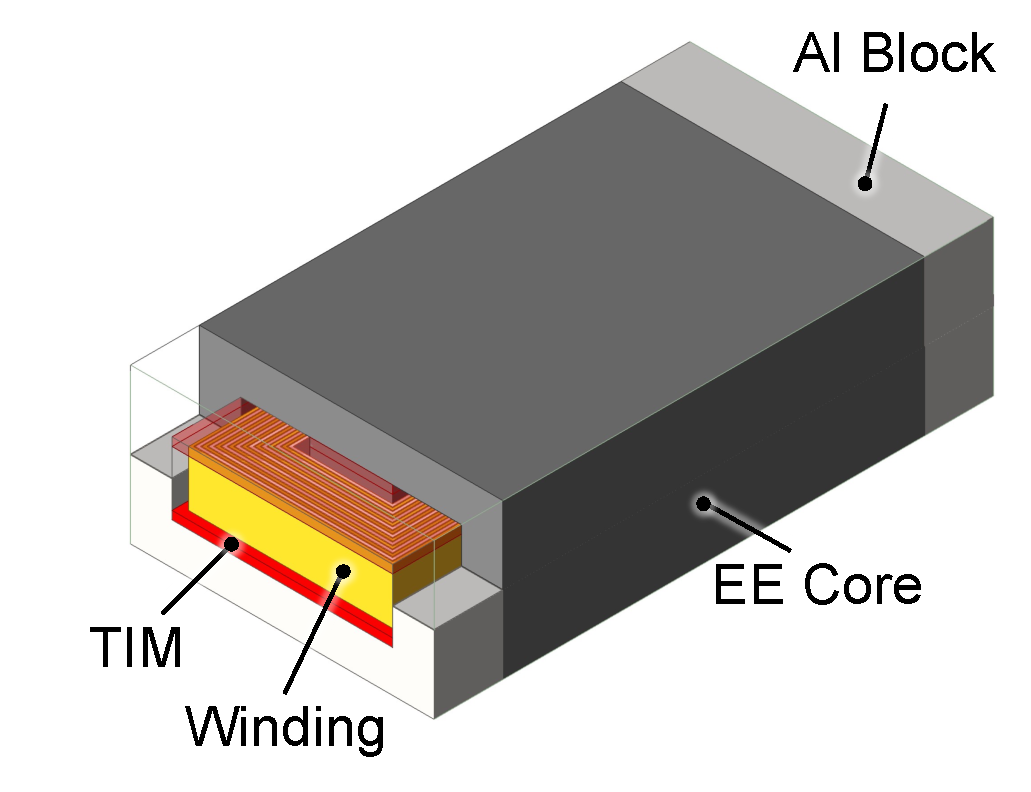
\includegraphics[width=0.5\columnwidth]{figures_chapter4/flatwise_simmodel.pdf}
        \label{fig:sim_model_flatwise}
    }
    \caption{Simulation models used of the (a) edgewise-wound (conventional) and (b) flatwise-wound (proposed) transformers.}
    \label{fig:simmodels}
\end{figure}

It is to be noted that the electromagnetic losses were coupled one-way into Ansys Icepak for the steady-state thermal analysis. This unidirectional coupling was deliberately selected to maintain a straightforward comparative baseline. While ferrite core losses are temperature-dependent, this characteristic varies significantly among different materials and introduces unnecessary complexity for a relative evaluation. 

\subsection{Electrostatic Simulation Conditions}
Electrostatic simulation using Ansys Maxwell was performed to evaluate if the transformer will avoid breakdown in operating conditions. To evaluate the isolation performance, designers set the secondary side voltage to 0 V (grounded) and assign a test DC voltage according to industry standard. Since the transformers in this study are a small-scale version of their counterparts, test voltages of 100 V and 200 V are applied to the primary side. The Electrostatic Solver was used for this set of simulations. A 2D simulation was utilized in this context since the transformer facial profile is symmetric around its geometry. The model used in the setup is shown in Figure \ref{fig:v_edge}a and \ref{fig:v_flat}a for the edgewise and flatwise configurations respectively.

\subsection{Thermal Simulation Conditions}
Steady-state Thermal simulation using Ansys Icepak was performed to evaluate the 3D steady-state spatial temperature distribution of the transformers. Two distinct thermal scenarios were evaluated. The losses from the electromagnetic simulation are coupled to their corresponding parts. First, natural air cooling was simulated to assess the intrinsic thermal performance of each transformer. This simply meant not applying any convection boundaries to the surfaces. Second, a forced air cooling scenario was modeled to represent practical operating conditions where the largest surface area of the transformer is mounted on a heat sink. This was implemented by applying a convective heat transfer coefficient of $h=$ 50 W/$(\text{m}^2\cdot K)$ to the bottom face of an aluminum block. The ambient temperature is set at 25.0$^\circ$C. The silicon-based TIM between the core and the windings has a thermal conductivity of 10 W/$(\text{m}\cdot K)$. A TIM with the same conductivity is also added as an interface between the bottom face of the transformer and the aluminum block. An example simulation model for the forced-air cooling setup is shown in Figure \ref{fig:forced_airsetup}.

\begin{figure}[h!]
    \centering
        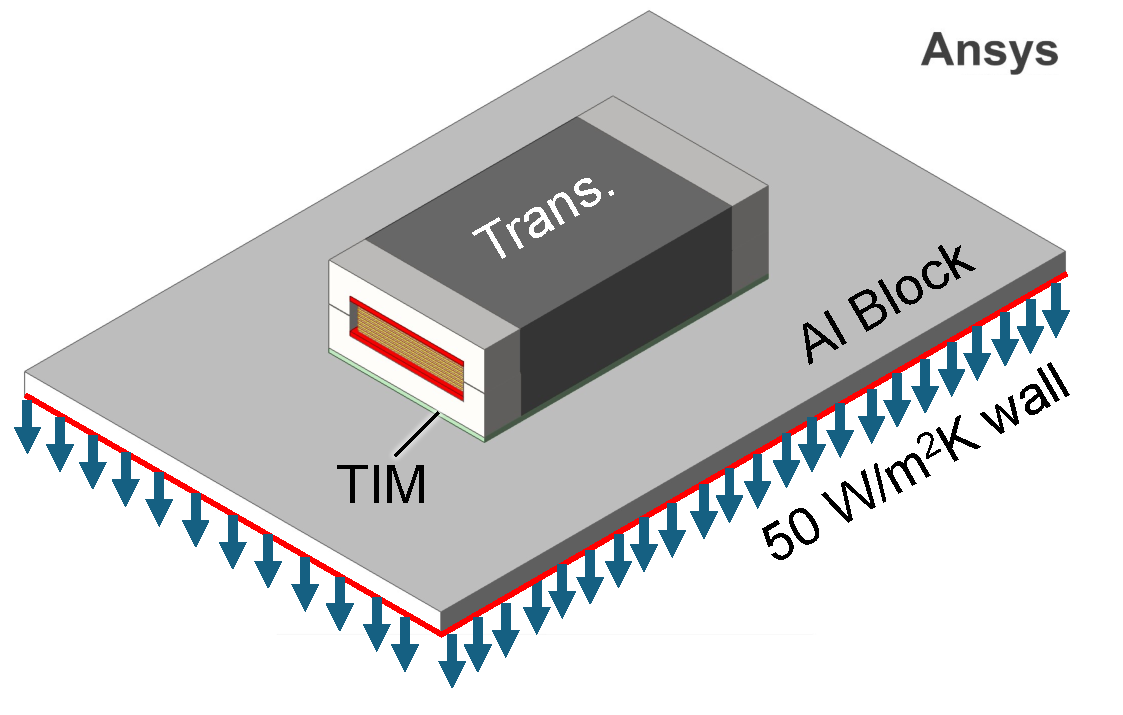
\includegraphics[width=0.5\columnwidth]{figures_chapter4/simsetup_forcedair.pdf}%
    \caption{Simulation model for the forced-air cooling scenario, as demonstrated on the edgewise-wound transformer.}
    \label{fig:forced_airsetup}
\end{figure}

\section{Simulation Results}

\subsection{Electromagnetic Simulation Results}
The electromagnetic simulation results at the operating frequency of 28.5 kHz are presented in Figure \ref{fig:bj_edge}a and Figure \ref{fig:bj_flat}a respectively. A close-up of the Magnetic Flux Density $B$ plots are shown in Figure \ref{fig:bj_edge}b and Figure \ref{fig:bj_flat}b respectively. A close-up of the Current Density $J$ plots are shown in Figure \ref{fig:bj_edge}c and Figure\ref{fig:bj_flat}c.

\begin{figure}[h!]
    \centering
        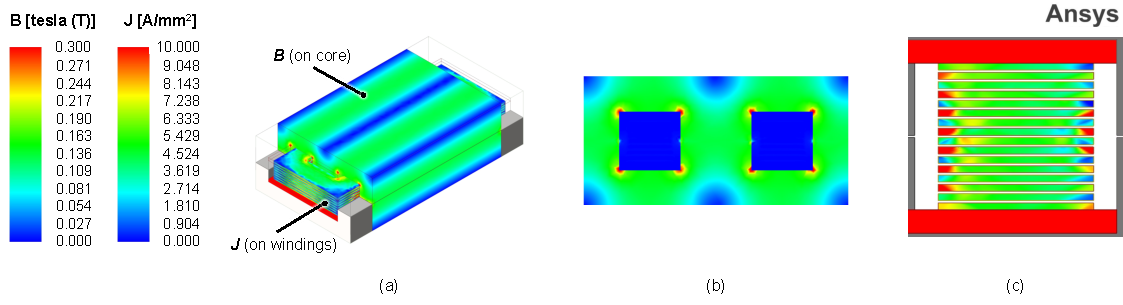
\includegraphics[width=\columnwidth]{figures_chapter4/bj_simresults_edgewise.pdf}%
    \caption{Electromagnetic simulation results for the edgewise-wound transformer: (a) $B$ and $J$ plots together, (b) close-up of $B$ plot, and (c) close-up of $J$ plot.}
    \label{fig:bj_edge}
\end{figure}

\begin{figure}[h!]
    \centering
        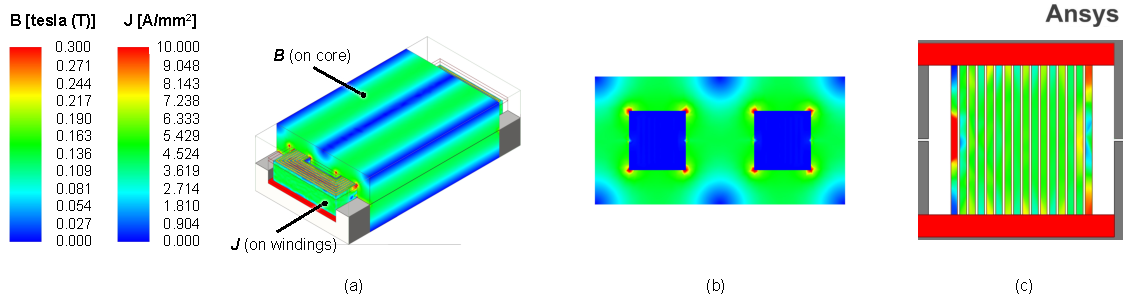
\includegraphics[width=\columnwidth]{figures_chapter4/bj_simresults_flatwise.pdf}%
    \caption{Electromagnetic simulation results for the flatwise-wound (proposed) transformer: (a) $B$ and $J$ plots together, (b) close-up of $B$ plot, and (c) close-up of $J$ plot.}
    \label{fig:bj_flat}
\end{figure}

The obtained magnetizing inductances are 200.14 $\upmu$H and 200.93 $\upmu$H for the edgewise and flatwise-wound transformers respectively, validating the $L_m$ design given the chosen parameters. The expected behaviors of the Magnetic Flux Density $B$ are seen and both transformers are not saturated. Moreover, the current density distribution is also expected, as current tends to crowd where the H-field is more prominent, which is towards the air gaps.  

\subsection{Electrostatic Simulation Results}\label{sec:breakdown}
The electrostatic simulation setups for the edgewise-wound and flatwise-wound (proposed) transformers are shown in Figure \ref{fig:v_edge}a and Figure \ref{fig:v_flat}a respectively. A 2D cross-section representing one window is taken as the simulation environment. The electric-field $E$ plots at 100 V test voltage are shown in Figure \ref{fig:v_edge}b and Figure \ref{fig:v_flat}b for the edgewise-wound and flatwise-wound transformers respectively. The $E$ plots at 200 V test voltage are shown in Figure \ref{fig:v_edge}c and Figure \ref{fig:v_flat}c for the edgewise-wound and flatwise-wound transformers respectively. As seen from the $E$ plots, the chosen $d_\mathrm{inter}$ is able to stand up to 200 V without causing electrical breakdown. There are some hotspots towards the intersection of air and the wires, and also at the triple point of the air, TIM, and the wire, but these do not reach the threshold.  

\begin{figure}[h!]
    \centering
        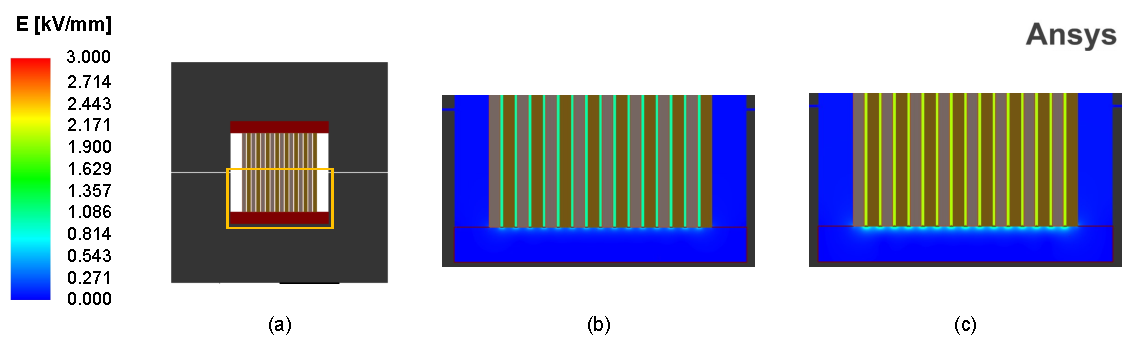
\includegraphics[width=\columnwidth]{figures_chapter4/efield_simresults_edgewise.pdf} 
    \caption{Electrostatic simulation (a) setup and results for the edgewise-wound transformer: (b) 100 V test voltage, and (c) 200 V test voltage.}
    \label{fig:v_edge}
    
\end{figure}

\begin{figure}[h!]
    \centering
        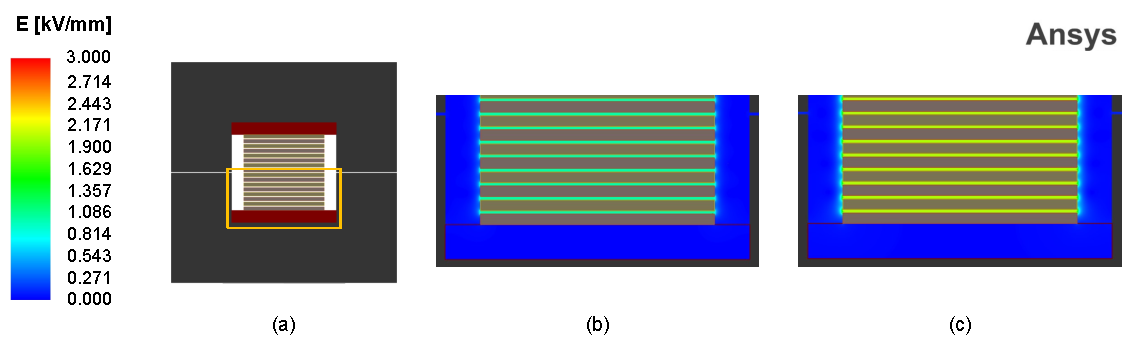
\includegraphics[width=\columnwidth]{figures_chapter4/efield_simresults_flatwise.pdf}
    \caption{Electrostatic simulation (a) setup and results for the flatwise-wound (proposed) transformer: (b) 100 V test voltage, and (c) 200 V test voltage.}
     \label{fig:v_flat}
    
\end{figure}

\subsection{Thermal Simulation Results} 
The thermal simulation results at the operating frequency of 28.5 kHz are presented in Figure \ref{fig:temp_natural}. Under the natural cooling scenario, the edgewise-wound transformer, as shown in Figure \ref{fig:temp_natural}, confirms the predicted thermal bottleneck; the inefficient series thermal path leads to localized heat accumulation in the windings, resulting in a significantly higher peak temperature of 66.9$^\circ$C. In contrast, the proposed flatwise-wound transformer, as shown in Figure \ref{fig:temp_natural}b, demonstrates superior thermal stability, exhibiting a uniform heat distribution and a peak temperature of approximately 56.0$^\circ$C. This discrepancy confirms that the flatwise structure offers a lower internal thermal resistance, thereby validating the heat extraction principles discussed in Section \ref{section:heat_dissipation}.

\begin{figure}[h!]
    \centering
        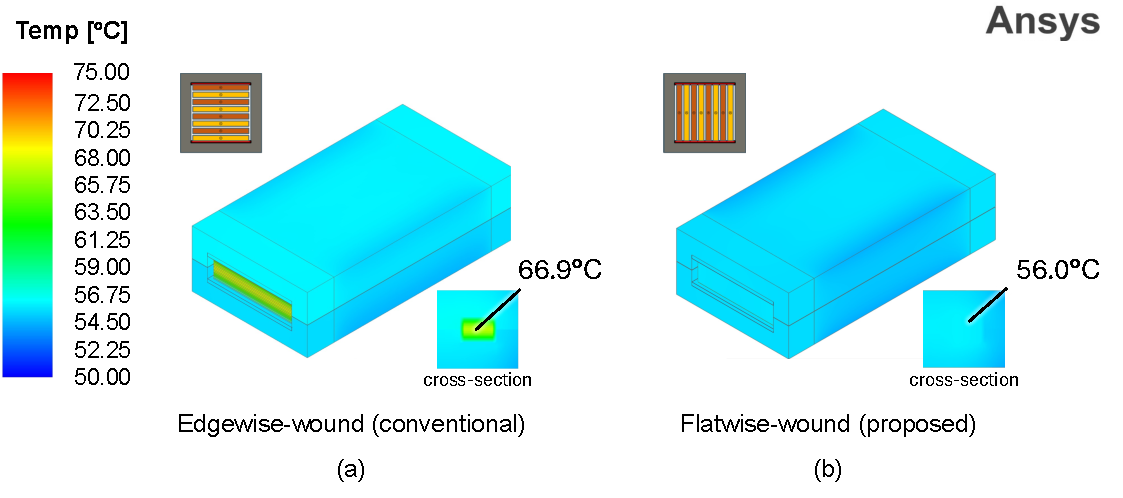
\includegraphics[width=\columnwidth]{figures_chapter4/natural_simresults.pdf}%
    \caption{Thermal simulation results of the (a) edgewise-wound and (b) flatwise-wound (proposed) transformers examined at 28.5 kHz, under natural cooling, at 25.0$^\circ$C ambient temperature.}
    \label{fig:temp_natural}
\end{figure}
The forced-air cooling scenario further amplifies this advantage. The edgewise-wound transformer as shown in Figure \ref{fig:temp_forced}a, continues to exhibit heat trapping within the central winding layers, resulting in a peak of 43.6$^\circ\text{C}$. Conversely, the flatwise model as shown in Figure \ref{fig:temp_forced}b, maintains a remarkably low peak temperature of approximately 30.2$^\circ\text{C}$ with a uniform gradient. These results highlight the scalable thermal advantage of the flatwise structure, demonstrating its effectiveness when integrated with practical cooling schemes. 

\begin{figure}[h!]
    \centering
    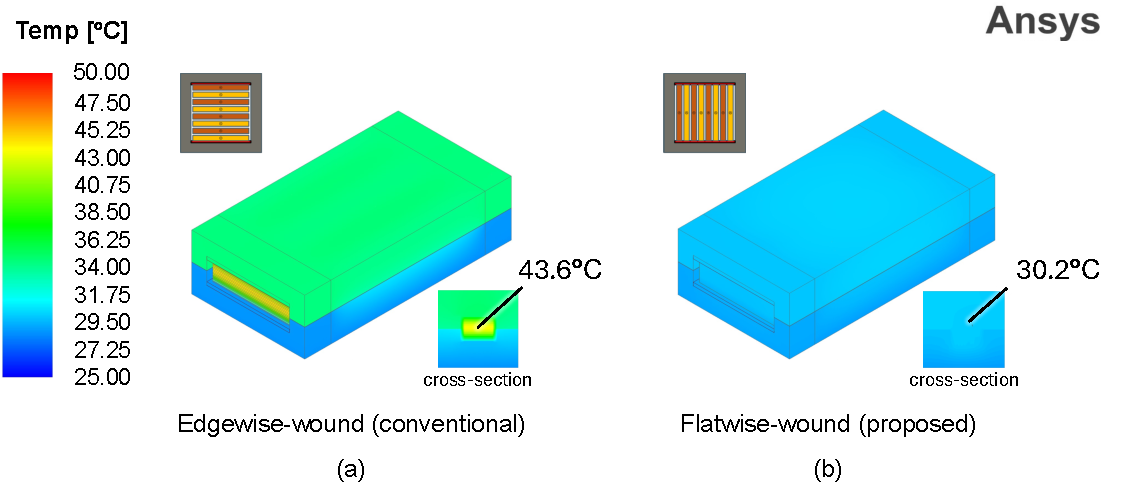
\includegraphics[width=\columnwidth]{figures_chapter4/forced_simresults.pdf}%
    \caption{Thermal simulation results of the (a) edgewise-wound and (b) flatwise-wound (proposed) transformers examined at 28.5 kHz, under forced-air cooling, at 25.0$^\circ$C ambient temperature.}
    \label{fig:temp_forced}
\end{figure}

\subsection{Electrical Properties and Losses}
The electrical properties derived from the simulation are summarized in Table \ref{tab:loss_comparison}. The comparison demonstrates that both winding configurations exhibit highly comparable electrical characteristics. The flatwise structure incurs only a marginal increase in winding loss (2.33 W vs. 2.24 W) and interwinding capacitance (1.72 nF vs. 1.45 nF) compared to its edgewise counterpart. Despite this very small penalty in total power loss ($+$2.5\%), the flatwise structure achieves a drastically lower peak temperature and uniform heat distribution capability, demonstrating that the benefit of reduced internal thermal resistance far outweighs the minor increase in electrical loss. More characterization on the effect of each configuration to the parasitics is a highly recommended next step of the research.

\begin{table}[H]
    \caption{Electrical Properties and Losses of the Simulated Transformers}
    \centering
    % Auto-fits table to column width
    
        \begin{tabular}{ccccc}
            \hline
            \textbf{Parameter} & \textbf{Symbol} & \textbf{Flatwise (prop.)} & \textbf{Edgewise} & \textbf{Unit} \\
            \hline \hline
            Interwinding Capacitance & $C_{\mathrm{ps}}$ & 1.72 & 1.45 & nF \\
            Leakage Inductance & $L_{\mathrm{lk}}$ & 0.04 & 0.02 & $\upmu$H \\
            \hline
            Core Loss & $P_{\mathrm{core}}$ & 0.87 & 0.87 & W \\
            Winding Loss & $P_{\mathrm{wind}}$ & 2.33 & 2.24 & W \\
            Aluminum Loss & $P_{\mathrm{Al}}$ & 0.09 & 0.09 & W \\
            \textbf{Total Loss} & \textbf{$P_{\mathrm{total}}$} & \textbf{3.29} & \textbf{3.21} & \textbf{W} \\
            \hline
        \end{tabular}%
    
    \label{tab:loss_comparison}
\end{table}

\chapter{Experimental Evaluation}
To experimentally validate the thermal performance of the two winding orientations, representative physical prototypes of the edgewise-wound and flatwise-wound transformers were fabricated. This section details the thermal performance comparison of the proposed and conventional-wound structures under steady-state operation in full load by examining key spots in the transformers. Moreover, the system-level efficiency with the two transformers is also quantified.
\section{Prototype Construction}
Representative physical prototypes of the edgewise-wound and flatwise-wound transformers were fabricated. To ensure a direct geometric comparison, Tr2E and Tr2F were selected as the edgewise-wound and flatwise-wound prototypes since they feature a square window area. The manufactured edgewise-wound prototype for Tr2E and its cross-section is shown in Figures \ref{fig:edgewise_3D} and \ref{fig:edgewise_cross} respectively. The manufactured flatwise-wound prototype for Tr2F and its cross-section is shown in Figure \ref{fig:flatwise_3D} and Figure \ref{fig:flatwise_cross} respectively. 

\begin{figure}[h!]
    \centering
    \subfloat[]{
        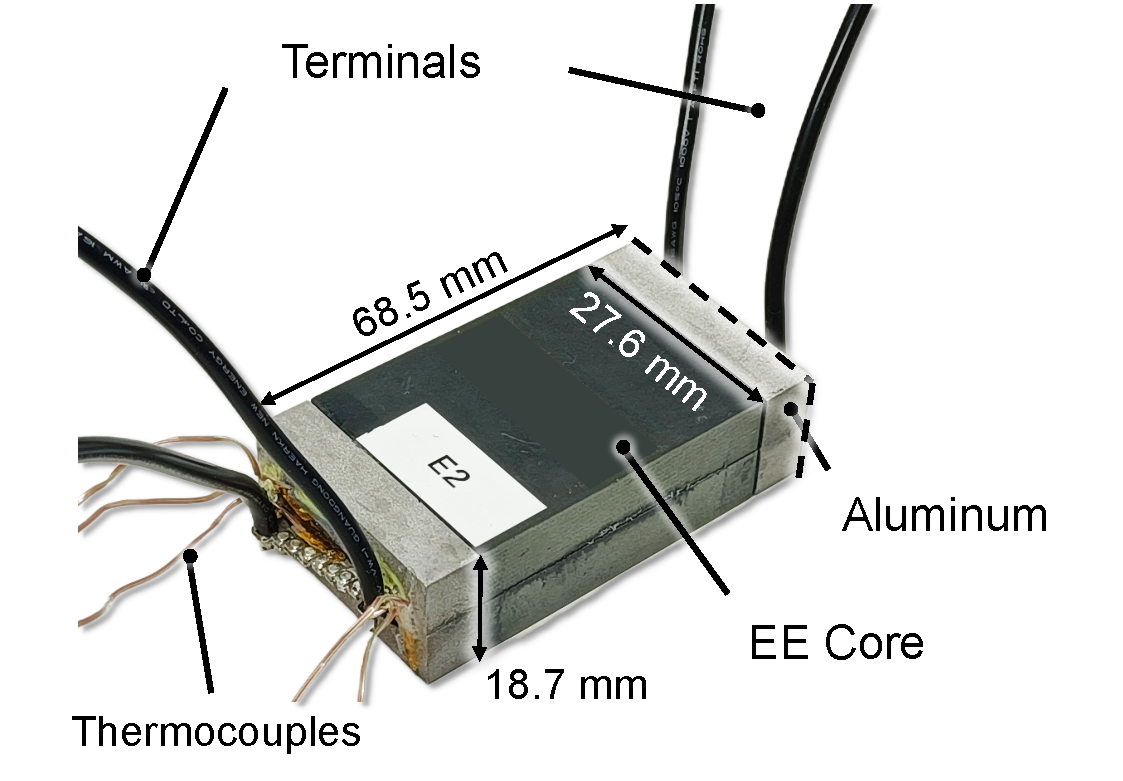
\includegraphics[width=0.5\columnwidth]{figures_chapter5/edgewise_3D_prototype.pdf}%
        \label{fig:edgewise_3D}
    }
    \subfloat[]{
        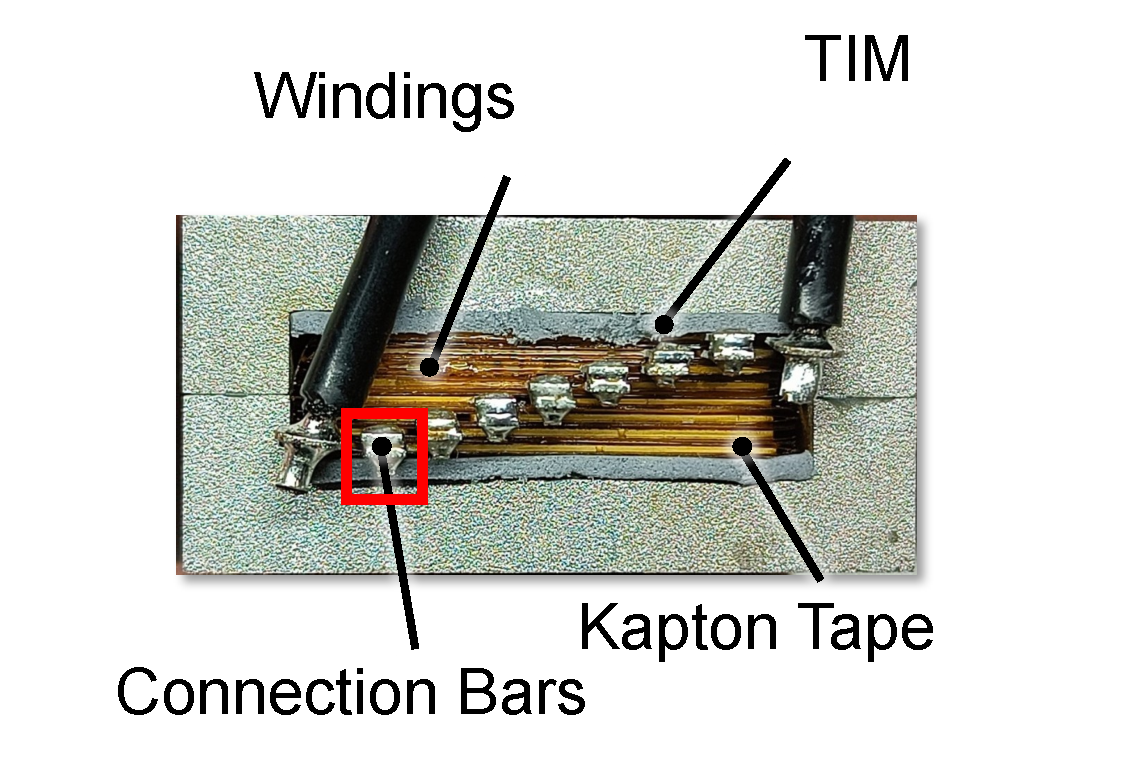
\includegraphics[width=0.5\columnwidth]{figures_chapter5/edgewise_cross_prototype.pdf}
        \label{fig:edgewise_cross}
    }
    \caption{(a) Prototype edgewise-wound transformer representing Tr2E, (b) cross-section of the edgewise-wound transformer prototype. The manufacturing limitation of the prototype is shown with the red box.}
    \label{fig:edgewise}
\end{figure}

\begin{figure}[h!]
    \centering
    \subfloat[]{
        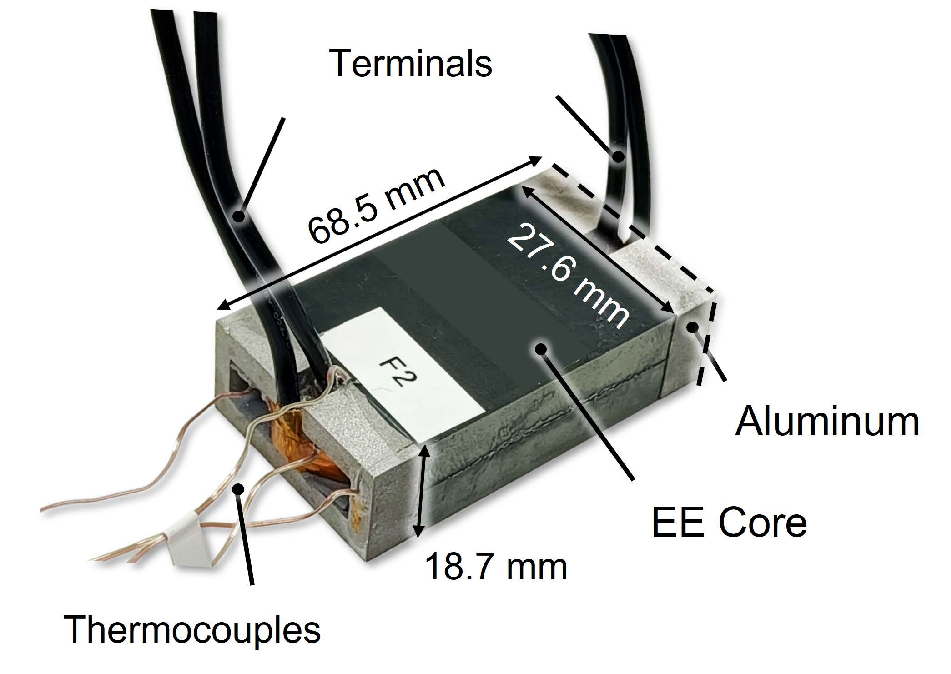
\includegraphics[width=0.5\columnwidth]{figures_chapter5/flatwise_3D_prototype.pdf}%
        \label{fig:flatwise_3D}
    }
    \subfloat[]{
        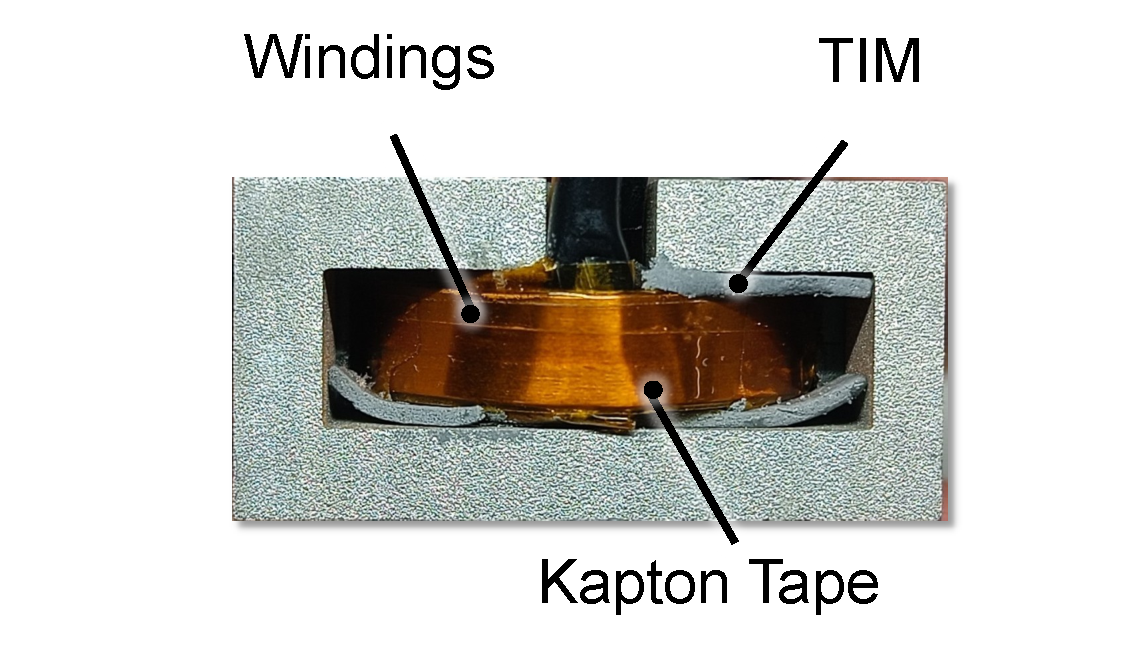
\includegraphics[width=0.5\columnwidth]{figures_chapter5/flatwise_cross_prototype.pdf}
        \label{fig:flatwise_cross}
    }
    \caption{(a) Prototype flatwise-wound transformer representing Tr2F, (b) cross-section of the flatwise-wound transformer prototype.}
    \label{fig:flatwise}
\end{figure}

Both prototypes utilize a custom-made LP10A ferrite EE-core with an air gap of 0.10 mm. To facilitate the supplementary heat extraction mechanisms defined in Section \ref{section:heat_dissipation}, DR-X100 (10 W/mK) was applied as the TIM between the core and the windings, and Al3031 aluminum blocks were fitted into the dead space. 

Several limitations arose during the fabrication of the prototypes. There were a few differences in the core dimensions and the wire dimensions as well due to the availability and capability of the custom manufacturability. 

For the conventional edgewise-wound transformer, strict spatial constraints dictated that the windings could not be continuously formed. Instead, the individual turn layers had to be connected and soldered in series using external connection bars that bridge the adjacent layers as shown in Figure \ref{fig:edgewise_cross}. For the flatwise-wound transformer, the continuous winding and folding process resulted in a curved profile at the bends as shown in Figure~\ref{fig:flatwise_cross}. This causes deviations in $d_\mathrm{clear}$ from the idealized simulated geometry. 

Furthermore, while the simulations modeled the inter-turn insulation solely as air, Kapton tape PF301 was applied to the physical windings to ensure dielectric safety in prolonged converter operation. Inherent assembly tolerances also introduced unintended changes in $d_{\mathrm{inter}}$ for both transformers, causing the turns to have unequal air gaps. These manufacturing steps naturally introduce physical imperfections compared to the idealized simulated designs, which are expected to cause deviations in the behaviors seen in the simulations. The detailed physical, magnetic, and electrical specifications at 28.5 kHz for each assembled transformer are summarized in Table \ref{tab:prototype_specs}.

\begin{table}[h!]
    \centering
    \caption{Specifications of the Prototype Transformers}
    
    \setlength{\tabcolsep}{3pt} % Reduces default space between columns
    \resizebox{\columnwidth}{!}{%
    \begin{tabular}{lccc}
    \hline
    \hline
    \textbf{Parameter} & \textbf{Symbol} & \textbf{Edgewise Prototype} & \textbf{Flatwise Prototype} \\
    \hline
    Magnetizing Inductance & $L_{\mathrm{m}}$ & 196.25 $\upmu$H & 196.97 $\upmu$H \\
    Conductor Dimensions & $w \times t$ & \multicolumn{2}{c}{6.00 $\times$ 0.30 mm}\\
    Number of Turns & $N_{\mathrm{p}} : N_{\mathrm{s}}$ & \multicolumn{2}{c}{8 : 8} \\
    Coupling Coefficient & $k$ & \multicolumn{2}{c}{0.9988} \\
    Air Gap & $l_{\mathrm{g}}$ & \multicolumn{2}{c}{0.10 mm} \\
    Window Area & $A_{\mathrm{win}}$ & {77.44 mm$^2$} & {76.56 mm$^2$} \\
    Window Aspect Ratio & $l_{\mathrm{win}}/w_{\mathrm{win}}$ & \multicolumn{2}{c}{$\sim$1.00} \\
    Transformer Dimensions & $l_{\mathrm{tr}} \times w_{\mathrm{tr}} \times h_{\mathrm{tr}}$ & \multicolumn{2}{c}{68.5 $\times$ 27.6 $\times$ 18.7 mm} \\
    Core Material & -- & \multicolumn{2}{c}{Ferrite LP10A} \\
    Core-to-Winding TIM & -- & \multicolumn{2}{c}{DR-X100 (10.0 W/(m$\cdot$K))} \\
    Dead Space Block & -- & \multicolumn{2}{c}{Al3031} \\
    \hline
    \hline
    \end{tabular}%
    }
    \label{tab:prototype_specs}
\end{table}

\section{Experimental Setup}
\subsection{Thermal Evaluation Setup}
Thermocouples were embedded on both transformer prototypes to capture the spatial thermal distribution, as illustrated in Figure \ref{fig:thermocouple}. The measurement nodes were selected to provide a comprehensive thermal profile. Specifically, the targeted measurement points included: the winding temperature $T_{\mathrm{wind}}$; the internal core window temperatures at the top and left side, $T_{\mathrm{top, in}}$ and $T_{\mathrm{left, in}}$; the exterior core temperatures $T_{\mathrm{top, out}}$, $T_{\mathrm{left, out}}$, and $T_{\mathrm{bot, out}}$; and the dead-space aluminum block temperature $T_{\mathrm{Al}}$.

\begin{figure}[h!]
    \centering
        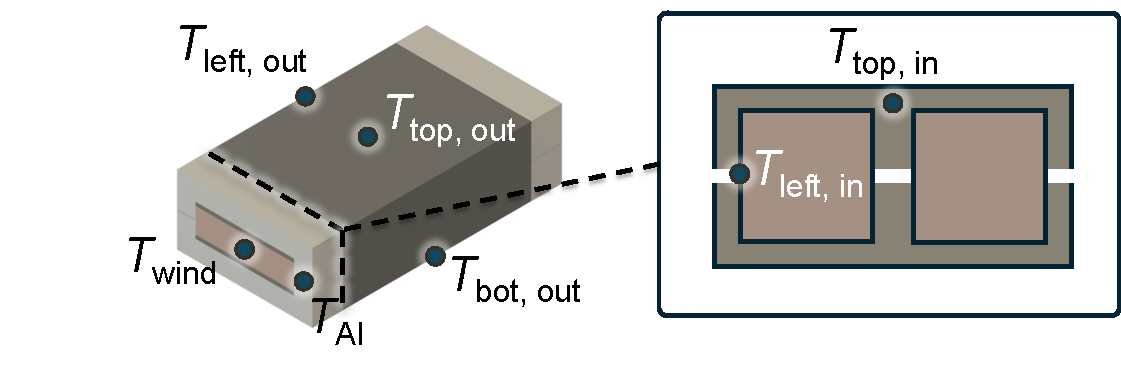
\includegraphics[width=0.85\columnwidth]{figures_chapter5/thermocouple.pdf}%
    \caption{Thermocouple placement for the measurement of key spots in the transformers. Thermocouples  $T_{\mathrm{left, out}}$, and $T_{\mathrm{bot, out}}$ are placed on the center of their respective faces as well.}
    \label{fig:thermocouple}
\end{figure}

Because the transformer geometry and internal heat generation are symmetric, thermocouple placement was concentrated on a single representative section to characterize the entire structure. This meant that the thermocouples on the respective internal and external faces indicated are placed on the center of their faces. The thermocouple for the winding was placed towards the middle, which meant between the fourth primary and secondary winding. The number of exterior sensors were minimized to prevent parasitic thermal mass and convection interference from skewing the thermal measurements. More insight into this is included in the Appendix: \nameref{app:longresult}.

The thermal evaluation was conducted under natural cooling and forced-air cooling through a heat sink. In the natural cooling setup depicted in Figure \ref{fig:natural}, the transformer was elevated on a wooden block. This low-thermal-conductivity boundary isolates the prototype by minimizing parasitic heat conduction through the bottom surface, ensuring that heat dissipation is only by natural convection to the surrounding ambient air. In the forced-air cooling configuration depicted in Figure \ref{fig:forcedair}, the transformers were physically coupled to an aluminum heatsink via a 1.00 mm TIM (ASKER C18 CPVS series, Kitagawa Industry Co., Ltd.) and subjected to active cooling from a 10.0-W fan. Across both test conditions, the thermal profiles were continuously recorded using a GRAPHTEC 200 data logger until an absolute thermal steady-state was achieved.

\begin{figure}[h!]
    \centering
    \subfloat[]{
        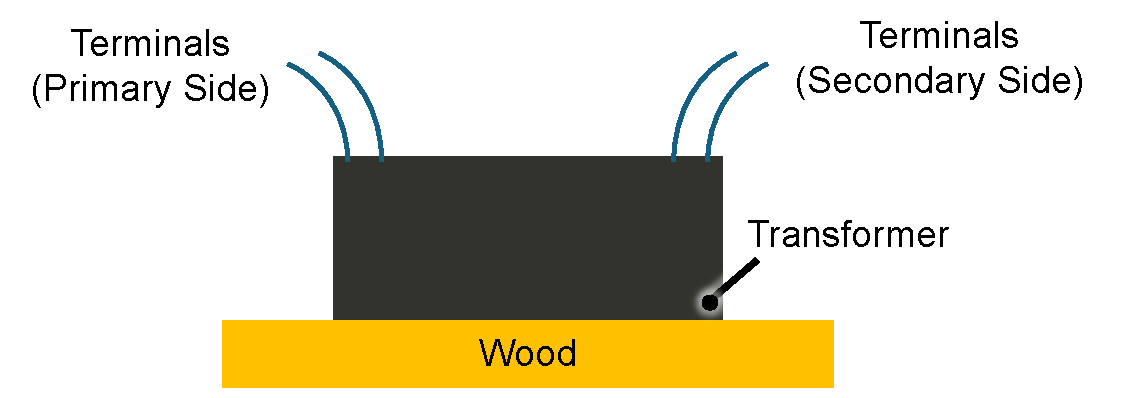
\includegraphics[width=0.8\columnwidth]{figures_chapter5/setup_natural.pdf}%
        \label{fig:natural}
    }

    \subfloat[]{
        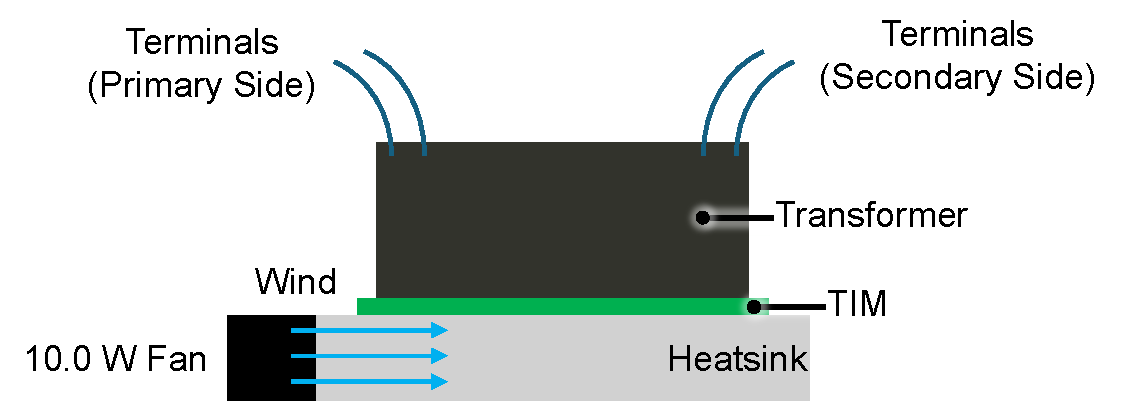
\includegraphics[width=0.8\columnwidth]{figures_chapter5/setup_forced.pdf}
        \label{fig:forcedair}
    }
    \caption{Cooling-setups for the transformers: (a) natural-cooling, (b) forced-air cooling through heat sink.}
    \label{fig:cooling setup}
\end{figure}
\pagebreak
\subsection{Experimental Environment and Implementation}
The prototyped transformers were evaluated in a 1-kW, 100-V CLLC converter operating at full load with a switching frequency of 28.5 kHz. The circuit diagram of the evaluation circuit and its photos are shown in Figures \ref{fig:circuitdiagram} and \ref{fig:converter} respectively. A diode bridge is placed instead in the secondary side for simplicity of the circuit operation. The specifications of the circuit are shown in Table \ref{tab:prototype_components}. 

\begin{figure}[h!]
    \centering
    \subfloat[]{
        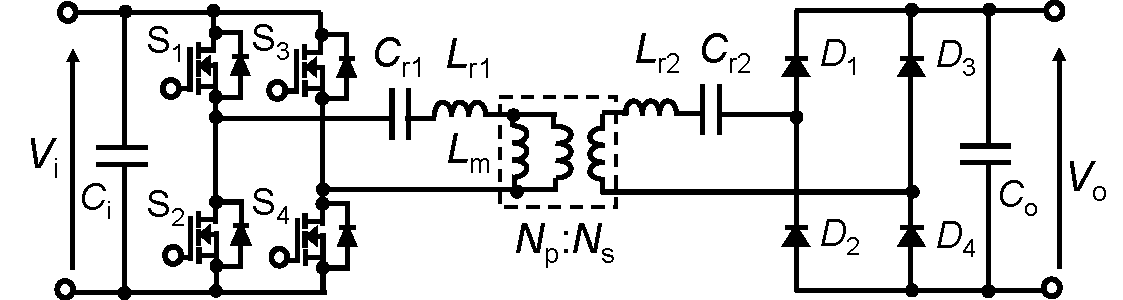
\includegraphics[width=\columnwidth]{figures_chapter5/circuitDiagram.pdf}%
        \label{fig:circuitdiagram}
    }

    \subfloat[]{
        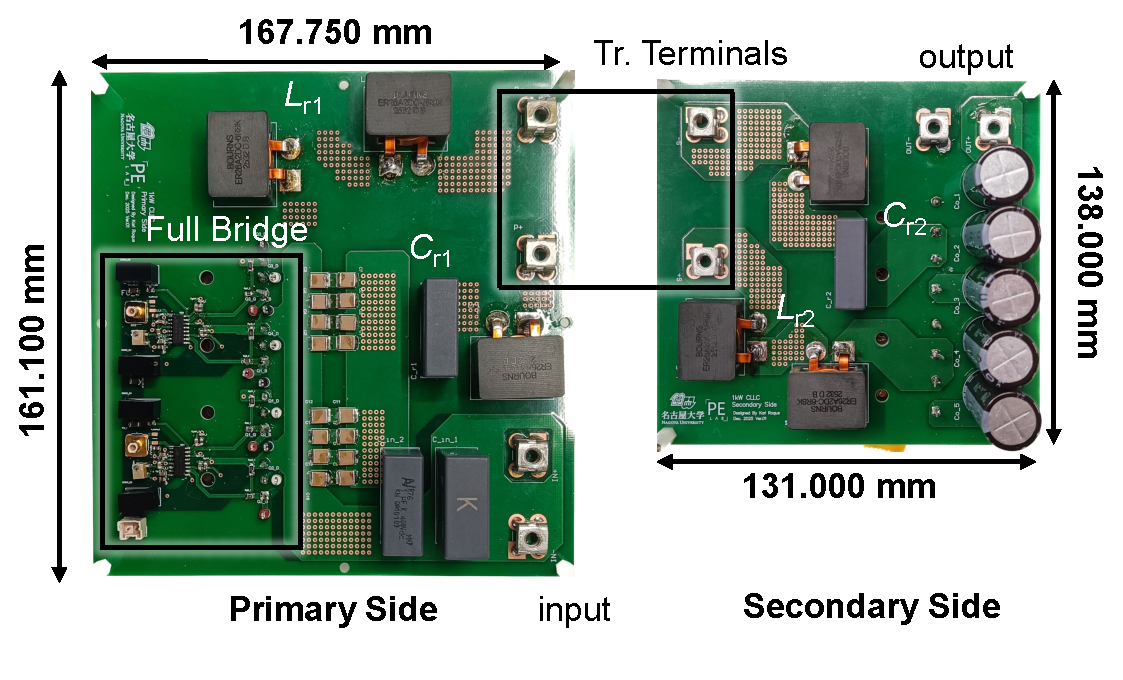
\includegraphics[width=0.8\columnwidth]{figures_chapter5/implementation_converter.pdf}
        \label{fig:converter}
    }
    \caption{(a) Circuit diagram of the manufactured 1-kW CLLC converter, (b) Photograph of the manufactured 1-kW CLLC converter.}
    \label{fig6}
\end{figure}
\begin{table}[h!]
\centering
\caption{Specifications and Components of the CLLC Resonant Converter Prototype}

\setlength{\tabcolsep}{3pt}
\resizebox{\textwidth}{!}{
\begin{tabular}{lcc}
\hline
\hline
\textbf{Parameter / Component} & \textbf{Symbol} & \textbf{Value / Part Number} \\
\hline
Input Voltage & $V_{\mathrm{i}}$ & 100 V \\
Output Voltage & $V_{\mathrm{o}}$ & 100 V \\
Maximum Rated Power & $P_{\mathrm{o}}$ & 1000 W \\
Switching Frequency & $f_{\mathrm{sw}}$ & 28.5 kHz \\
Resonant Frequency & $f_{\mathrm{r}}$ & 30.0 kHz \\
Dead Time & $t_\mathrm{d}$ & 360 ns\\
\hline
MOSFETs & $S_1, S_2, S_3, S_4$ & IPW65R050CFD7AXKSA1 \\
Half-Bridge Gate Driver & -- & SI8274GB4D-IS1 \\
Resonant Capacitors & $C_{\mathrm{r1}}, C_{\mathrm{r2}}$ & 1.4 $\upmu$F C4AQQBU4140M1WJ \\
Resonant Inductors & $L_{\mathrm{r1}}, L_{\mathrm{r2}}$ & 6.7 $\upmu$H ($\times 3$ in series) ER26A3DC-100K \\
Input Capacitors & $C_{\mathrm{in}}$ & \makecell{10 $\upmu$F R60MR51005040K \\ 1 $\upmu$F R76MR4100SE40K (in parallel)} \\
Secondary Side Diodes & $D_1, D_2, D_3, D_4$ & VX60202PW-M3/P \\
Output Capacitors & $C_{\mathrm{o}}$ & 100 $\upmu$F ($\times 5$ in parallel) 400HXW100MEFR12.5X40 \\
\hline
\hline
\end{tabular}%
}
\label{tab:prototype_components}


\end{table}

The experimental environment is shown in Figure \ref{fig:environment}. The transformer could have been isolated in a temperature-controlled environment, but this setup is chosen to mirror the possible set-up in the real-world application of the transformer. However, to isolate the thermal evaluation of the proposed transformers, the device under test (DUT) and its cooling system is put as far away as possible from the converter. An implementation of the natural and forced-air cooling scenario is shown in Figure \ref{fig:naturalaircooling} and \ref{fig:forcedaircooling} respectively.

\begin{figure}[h!]
    \centering
    
        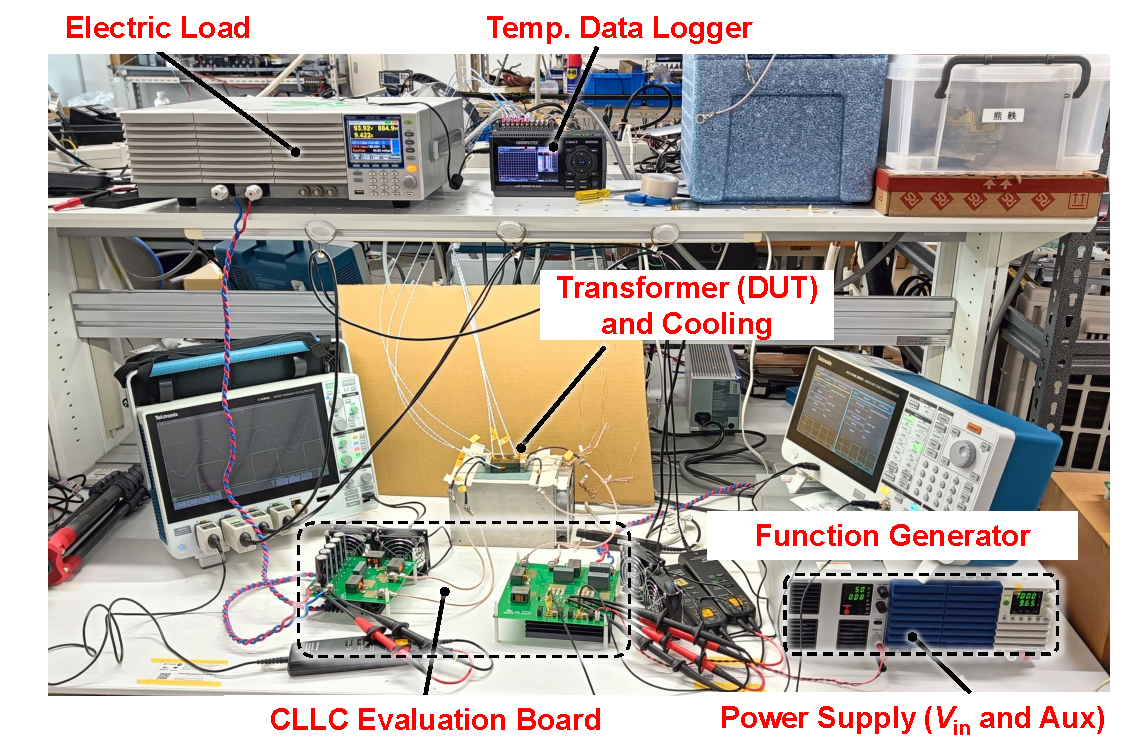
\includegraphics[width=\columnwidth]{figures_chapter5/implementation_workbench.pdf}%
        
    \caption{Experimental environment during the operational testing.}
    \label{fig:environment}
\end{figure}

\begin{figure}[h!]
    \centering
    \subfloat[]{
        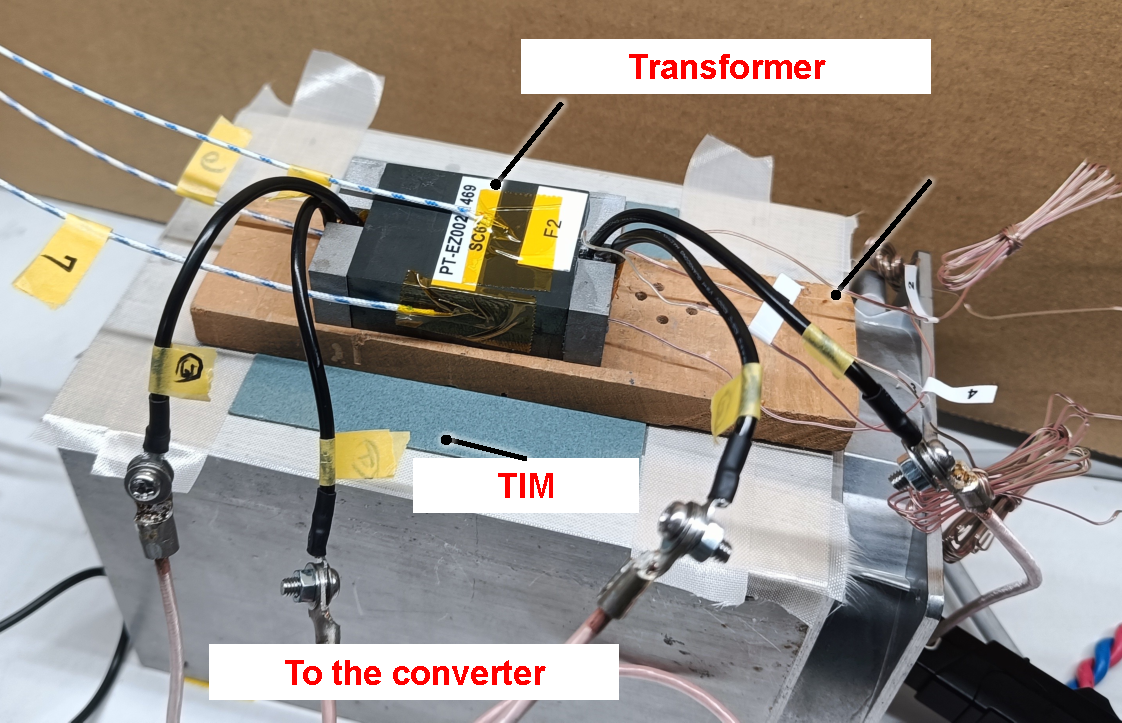
\includegraphics[width=0.7\columnwidth]{figures_chapter5/implementation_natralAir.pdf}%
        \label{fig:naturalaircooling}
    }

    \subfloat[]{
        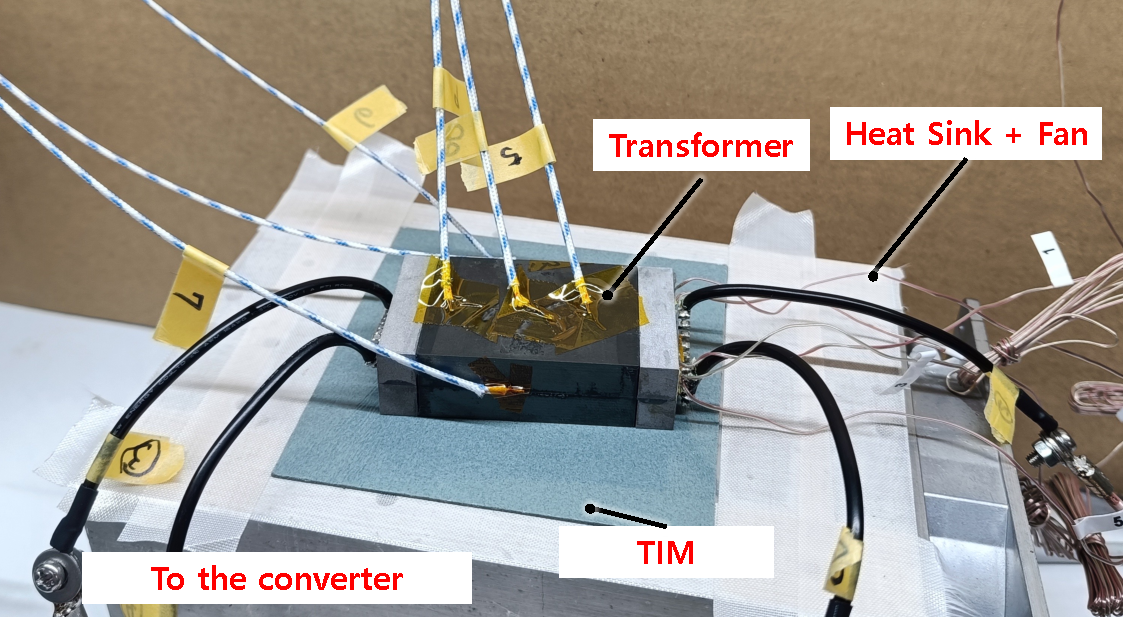
\includegraphics[width=0.7\columnwidth]{figures_chapter5/implementation_forcedAir.pdf}
        \label{fig:forcedaircooling}
    }
    \caption{Implementation of the cooling scenarios: (a) natural cooling, (b) forced-air cooling through heat sink.}
    \label{fig:imp}
\end{figure}


 Moreover, the equivalent AC resistance of each transformer was measured up to 300 kHz using a Keysight E4990A impedance analyzer from the primary side, with the secondary terminals shorted \cite{ref25}. The efficiency was also measured using a Hioki PW8001 Power Analyzer at intervals of 100 W from 100 to 1000 W. All equipment used in the experiment are detailed in Table \ref{tab:equipment}.

 \begin{table}[h!]
\centering
\caption{List of Equipment Used in the Experimental Setup}

\setlength{\tabcolsep}{3pt}
\begin{tabular}{ll}
\hline
\hline
\textbf{Equipment} & \textbf{Model / Manufacturer} \\
\hline
Oscilloscope & Tektronix MDO34 \\
Electric Load & Texio LSG-1050H \\
Function Generator & Tektronix AFG31102 \\
Power Analyzer & Hioki PW8001 + Hioki CT6841A\\
DC Power Supply & Kikusui PWR1201MH \\
AUX Power Supply (5V) & Matsusada TB160V15A720W \\
Differential Voltage Probe & Tektronix THDP0200 \\
Current Probe & Tektronix TCP0030A \\
\hline
\hline
\end{tabular}%

\label{tab:equipment}


\end{table}
 
\pagebreak
\section{Experimental Results}  
\subsection{AC Resistance Measurement Results}
Figure \ref{fig:ACResult} shows the prototype AC resistance profiles up to 300 kHz. At the operating frequency, the edgewise-wound transformer has a resistance of 32.47 m$\Omega$ while the flatwise-wound transformer has a resistance of 26.44 m$\Omega$. It seemed that the flatwise-wound transformer performed better in higher frequencies, but it is still inconclusive as the two transformers were not manufactured in exactly the same way. Further analysis is needed to quantify the winding loss performance of the two configurations. 
\begin{figure}[h!]
            \centering
            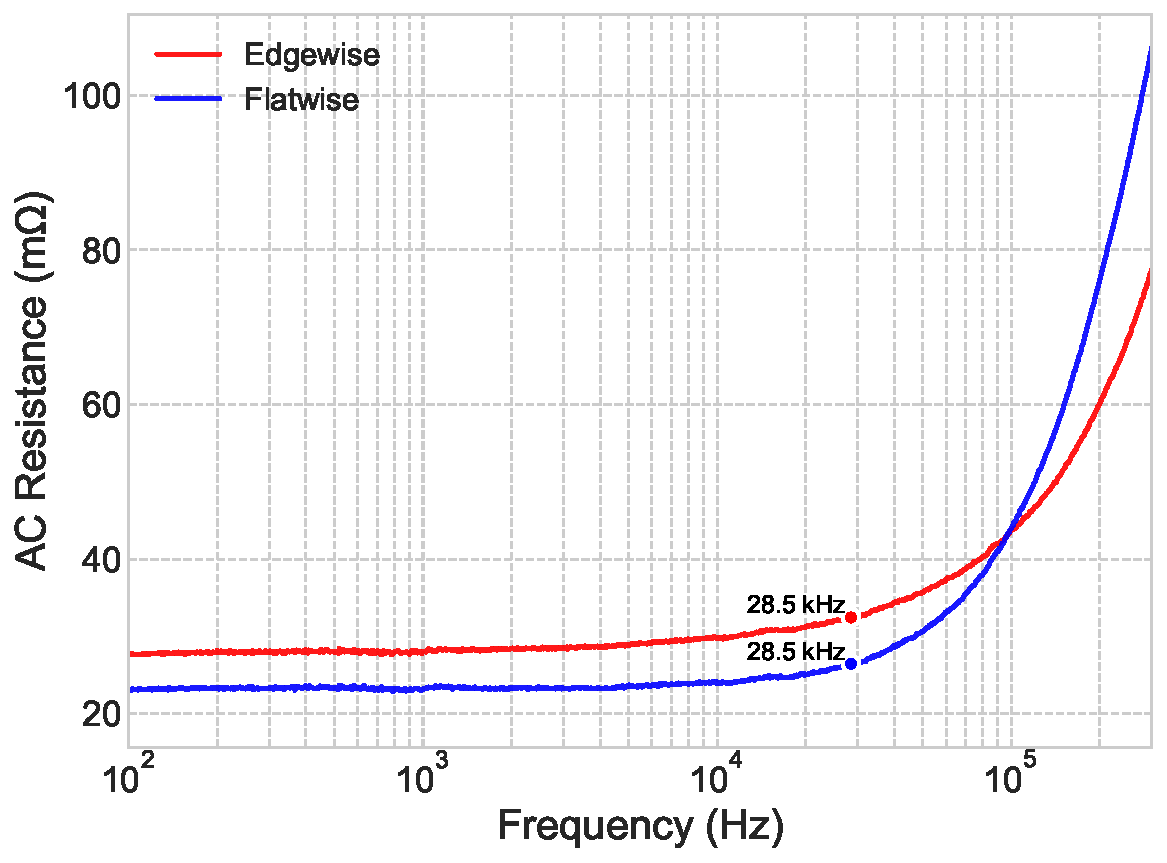
\includegraphics[width=0.7\columnwidth]{figures_chapter5/rs_short_circuit.pdf}
    \caption{AC Resistance profiles up to 300 kHz for the constructed prototypes.}
    \label{fig:ACResult}
\end{figure}
\pagebreak
\subsection{Operational Waveforms}
The zero-voltage switching (ZVS) experimental waveforms for the 1~kW CLLC converter operating at a 28.5~kHz switching frequency under natural and forced-air cooling are shown in Figure~\ref{fig:15}. Figure~\ref{fig:15a} and Figure~\ref{fig:15b} show the waveforms for the edgewise-wound and flatwise-wound transformer under natural cooling. Figure~\ref{fig:15c} and Figure~\ref{fig:15d} show the waveforms for the edgewise-wound and flatwise-wound transformer under forced-air cooling. Both the edgewise-wound and flatwise-wound prototypes demonstrate stable operation, with the primary side resonant current $i_{{\mathrm{r}_{\mathrm{pri}}}}$, output voltage $V_\mathrm{O}$, high-side gate voltage $V_\mathrm{gs}$, and drain-to-source voltage $V_\mathrm{ds}$ remaining well-regulated across both cooling conditions.
 
\begin{figure}[H]
\centering
% (a) Top circuit
        \subfloat[]{
        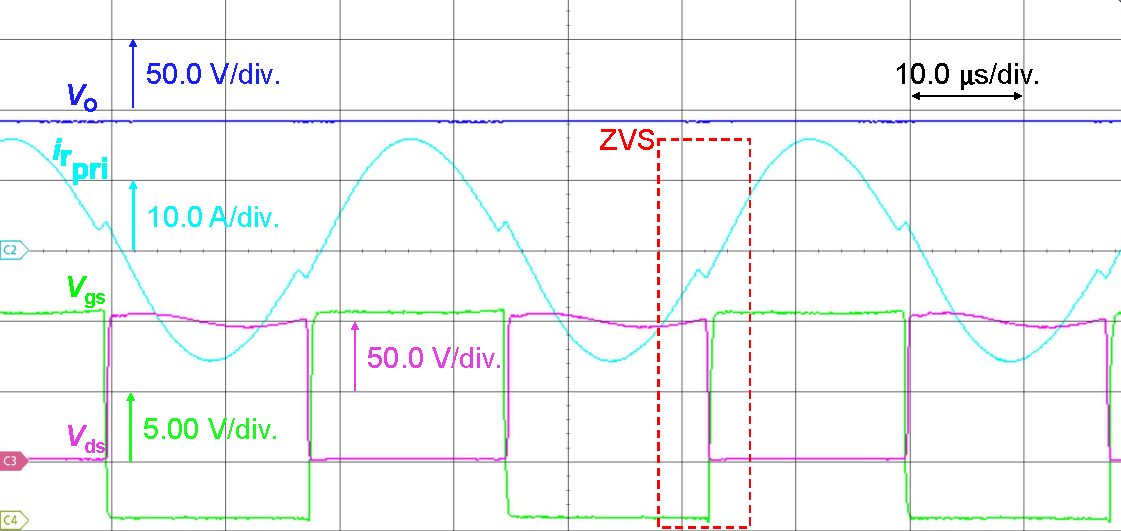
\includegraphics[width=0.7\columnwidth]{figures_chapter5/E2_natural.pdf} % Make sure this file exists
        \label{fig:15a}
        } 
        % This double backslash forces the next image to the line below (vertical stack)
        % (b) Middle circuit

        \subfloat[]{
        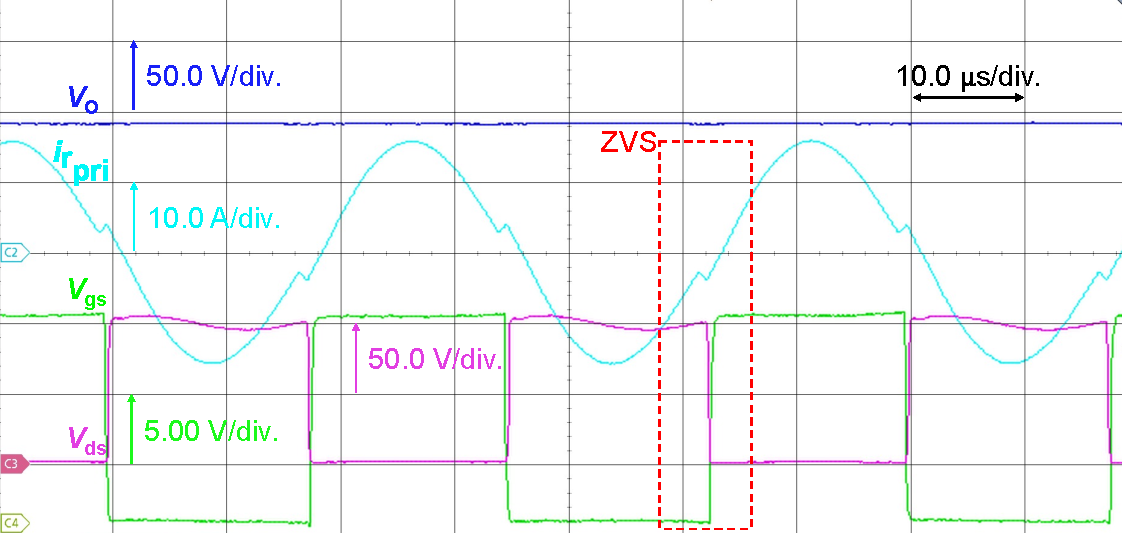
\includegraphics[width=0.7\columnwidth]{figures_chapter5/F2_natural.pdf}
        \label{fig:15b}
        }

        \subfloat[]{
        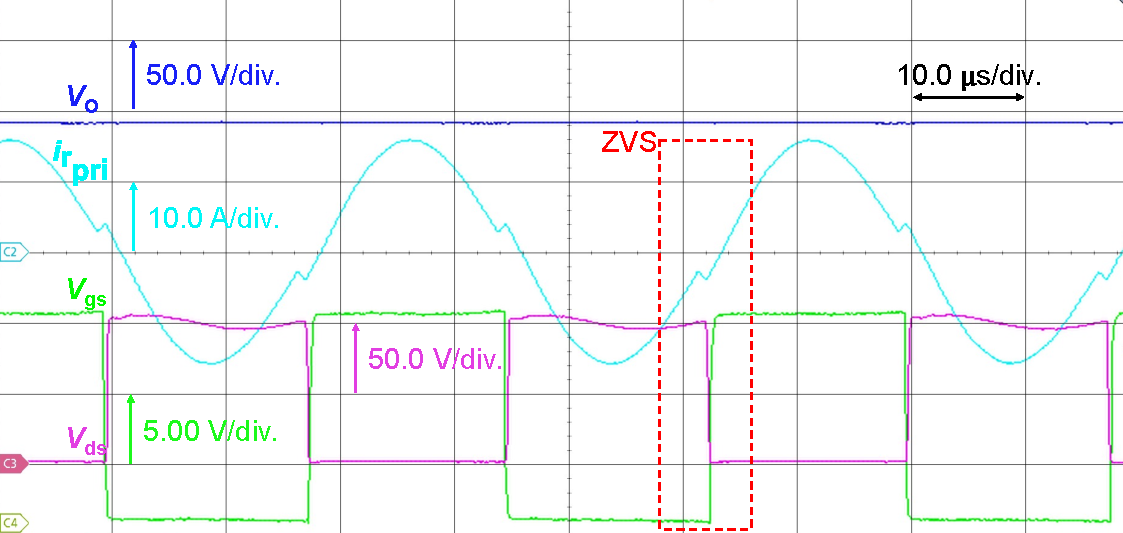
\includegraphics[width=0.7\columnwidth]{figures_chapter5/E2_forced.pdf} % Make sure this file exists
        \label{fig:15c}
        } 
        
        \subfloat[]{
        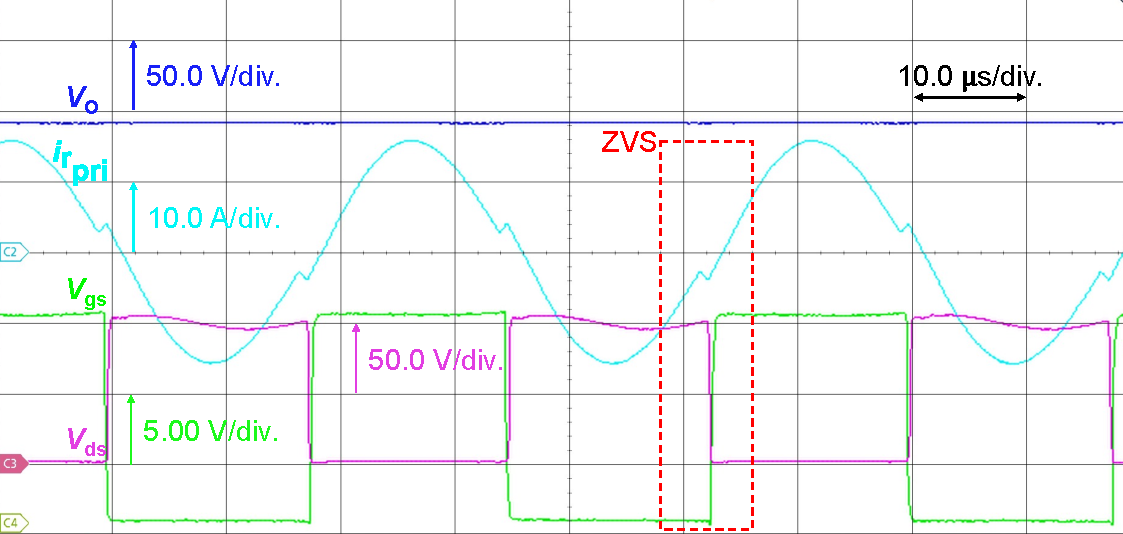
\includegraphics[width=0.7\columnwidth]{figures_chapter5/F2_forcedair.pdf}
        \label{fig:15d}
        } 
        \caption{Experimental waveforms of the transformers implemented in a 1-kW, 28.5-kHz CLLC at natural cooling: (a) edgewise-wound transformer, (b) flatwise-wound transformer; and forced-air cooling: (c) edgewise-wound transformer, (d) flatwise-wound transformer.}
        \label{fig:15}
\end{figure}

\pagebreak
\subsection{Temperature Profiles}
The measured temperature profiles of the edgewise and flatwise transformers during natural cooling are shown in Figure~\ref{fig:18}a and Figure~\ref{fig:18}b. As shown in the edgewise thermal profile, the temperature curve did not stabilize after one hour of continuous operation. To prevent thermal runaway, the test was aborted, recording a peak transient $T_{\mathrm{wind}}$ of 74.3$^{\circ}$C. The test for the flatwise transformer was also recorded for one hour and was able to stabilize at $T_{\mathrm{wind}}$ of 66.7$^{\circ}$C. Longer full-load results are available through a repeat test as shown in the Appendix: \nameref{app:longresult}.

In the natural cooling evaluation, both prototypes exhibited tight thermal coupling between the primary winding and the internal core window, shown by a 0.8 to 1.3$^{\circ}$C gradient between $T_{\mathrm{wind}}$ and $T_{\mathrm{top, in}}$, $T_{\mathrm{left, in}}$. However, in terms of the internal-to-external temperature gradient, the edgewise structure suffers from a 9.0$^{\circ}$C gradient between $T_{\mathrm{wind}}$ and $T_{\mathrm{top, out}}$, and a 13.4$^{\circ}$C gradient to $T_{\mathrm{left, out}}$, indicating internal heat entrapment. The flatwise structure reduces these internal-to-external gradients to 4.1$^{\circ}$C and 8.7$^{\circ}$C, respectively. This therefore proves that the flatwise structure is able to move heat easily from the inside to the outside, preventing heat from getting trapped inside the core.

Furthermore, the observed temperature hierarchy, indicated by $T_{\mathrm{wind}} > T_{\mathrm{top, in}}$, $T_{\mathrm{left, in}} > T_{\mathrm{top, out}} > T_{\mathrm{left, out}}$ aligns with the fundamental heat transfer mechanisms of the transformer. The internal winding serves as the primary heat source, leading to $T_{\mathrm{wind}}$ peaking. Consequently, $T_{\mathrm{top, in}}$, $T_{\mathrm{left, in}}$ maintain elevated temperatures necessary to overcome the thermal resistance of the ferrite core and facilitate outward conduction. At the exterior boundaries, the cooling efficiency is governed by natural convection. Heat dissipation at the top horizontal surface is constrained by the upward plume of heated air, which reduces the local convective heat transfer coefficient. Conversely, the vertical outer leg is exposed to a continuous buoyancy-driven flow of cooler ambient air. This then leads to $T_{\mathrm{top, out}} > T_{\mathrm{left, out}}$.

The advantage of the flatwise structure is further demonstrated during the forced-air cooling evaluation. Under forced-air cooling, the temperature profiles shown in Figure~\ref{fig:18}c and Figure~\ref{fig:18}d confirm that both prototypes reached a stable steady state. However, the edgewise $T_{\mathrm{wind}}$ stabilized at a higher temperature of 46.5$^{\circ}$C, whereas the flatwise $T_{\mathrm{wind}}$ maintained a cooler steady-state operating temperature of 41.5$^{\circ}$C. 

The active cooling system anchored $T_{\mathrm{bot, out}}$ at 31.1$^{\circ}$C and 31.3$^{\circ}$C for the edgewise and flatwise structures, respectively. The $T_{\mathrm{top, out}}$ for both structures was approximately 40.0$^{\circ}$C. However, the internal thermal distribution shows a clear difference in thermal resistance. The edgewise prototype had a 15.4$^{\circ}$C gradient between $T_{\mathrm{wind}}$ and $T_{\mathrm{bot, out}}$, and a 6.6$^{\circ}$C gradient between $T_{\mathrm{wind}}$ and $T_{\mathrm{top, out}}$. The flatwise prototype had a 10.2$^{\circ}$C gradient and a 1.3$^{\circ}$C gradient between $T_{\mathrm{wind}}$ and $T_{\mathrm{bot, out}}$, and $T_{\mathrm{top, out}}$, respectively. Additionally, the gradient between $T_{\mathrm{wind}}$ and $T_{\mathrm{Al}}$ was 3.4$^{\circ}$C for the flatwise prototype, compared to 5.7$^{\circ}$C for the edgewise prototype. Because the flatwise exterior temperatures closely match its interior winding temperature, these gradients prove the thermal advantage of the flatwise structure.

To summarize, with the flatwise-wound prototype, the peak winding temperature was reduced by 7.7$^{\circ}$C in natural cooling and 5.0$^{\circ}$C in forced air cooling. Moreover, the temperature gradients $T_{\mathrm{wind}} - T_{\mathrm{top, out}}$ and $T_{\mathrm{wind}} - T_{\mathrm{bot, out}}$ were reduced by 4.9$^{\circ}$C and 3.4$^{\circ}$C respectively under natural cooling conditions, and 5.2$^{\circ}$C and 5.3$^{\circ}$C respectively under forced-air cooling conditions.
\pagebreak
\begin{figure}[h!]
\centering
% (a) Left circuit
        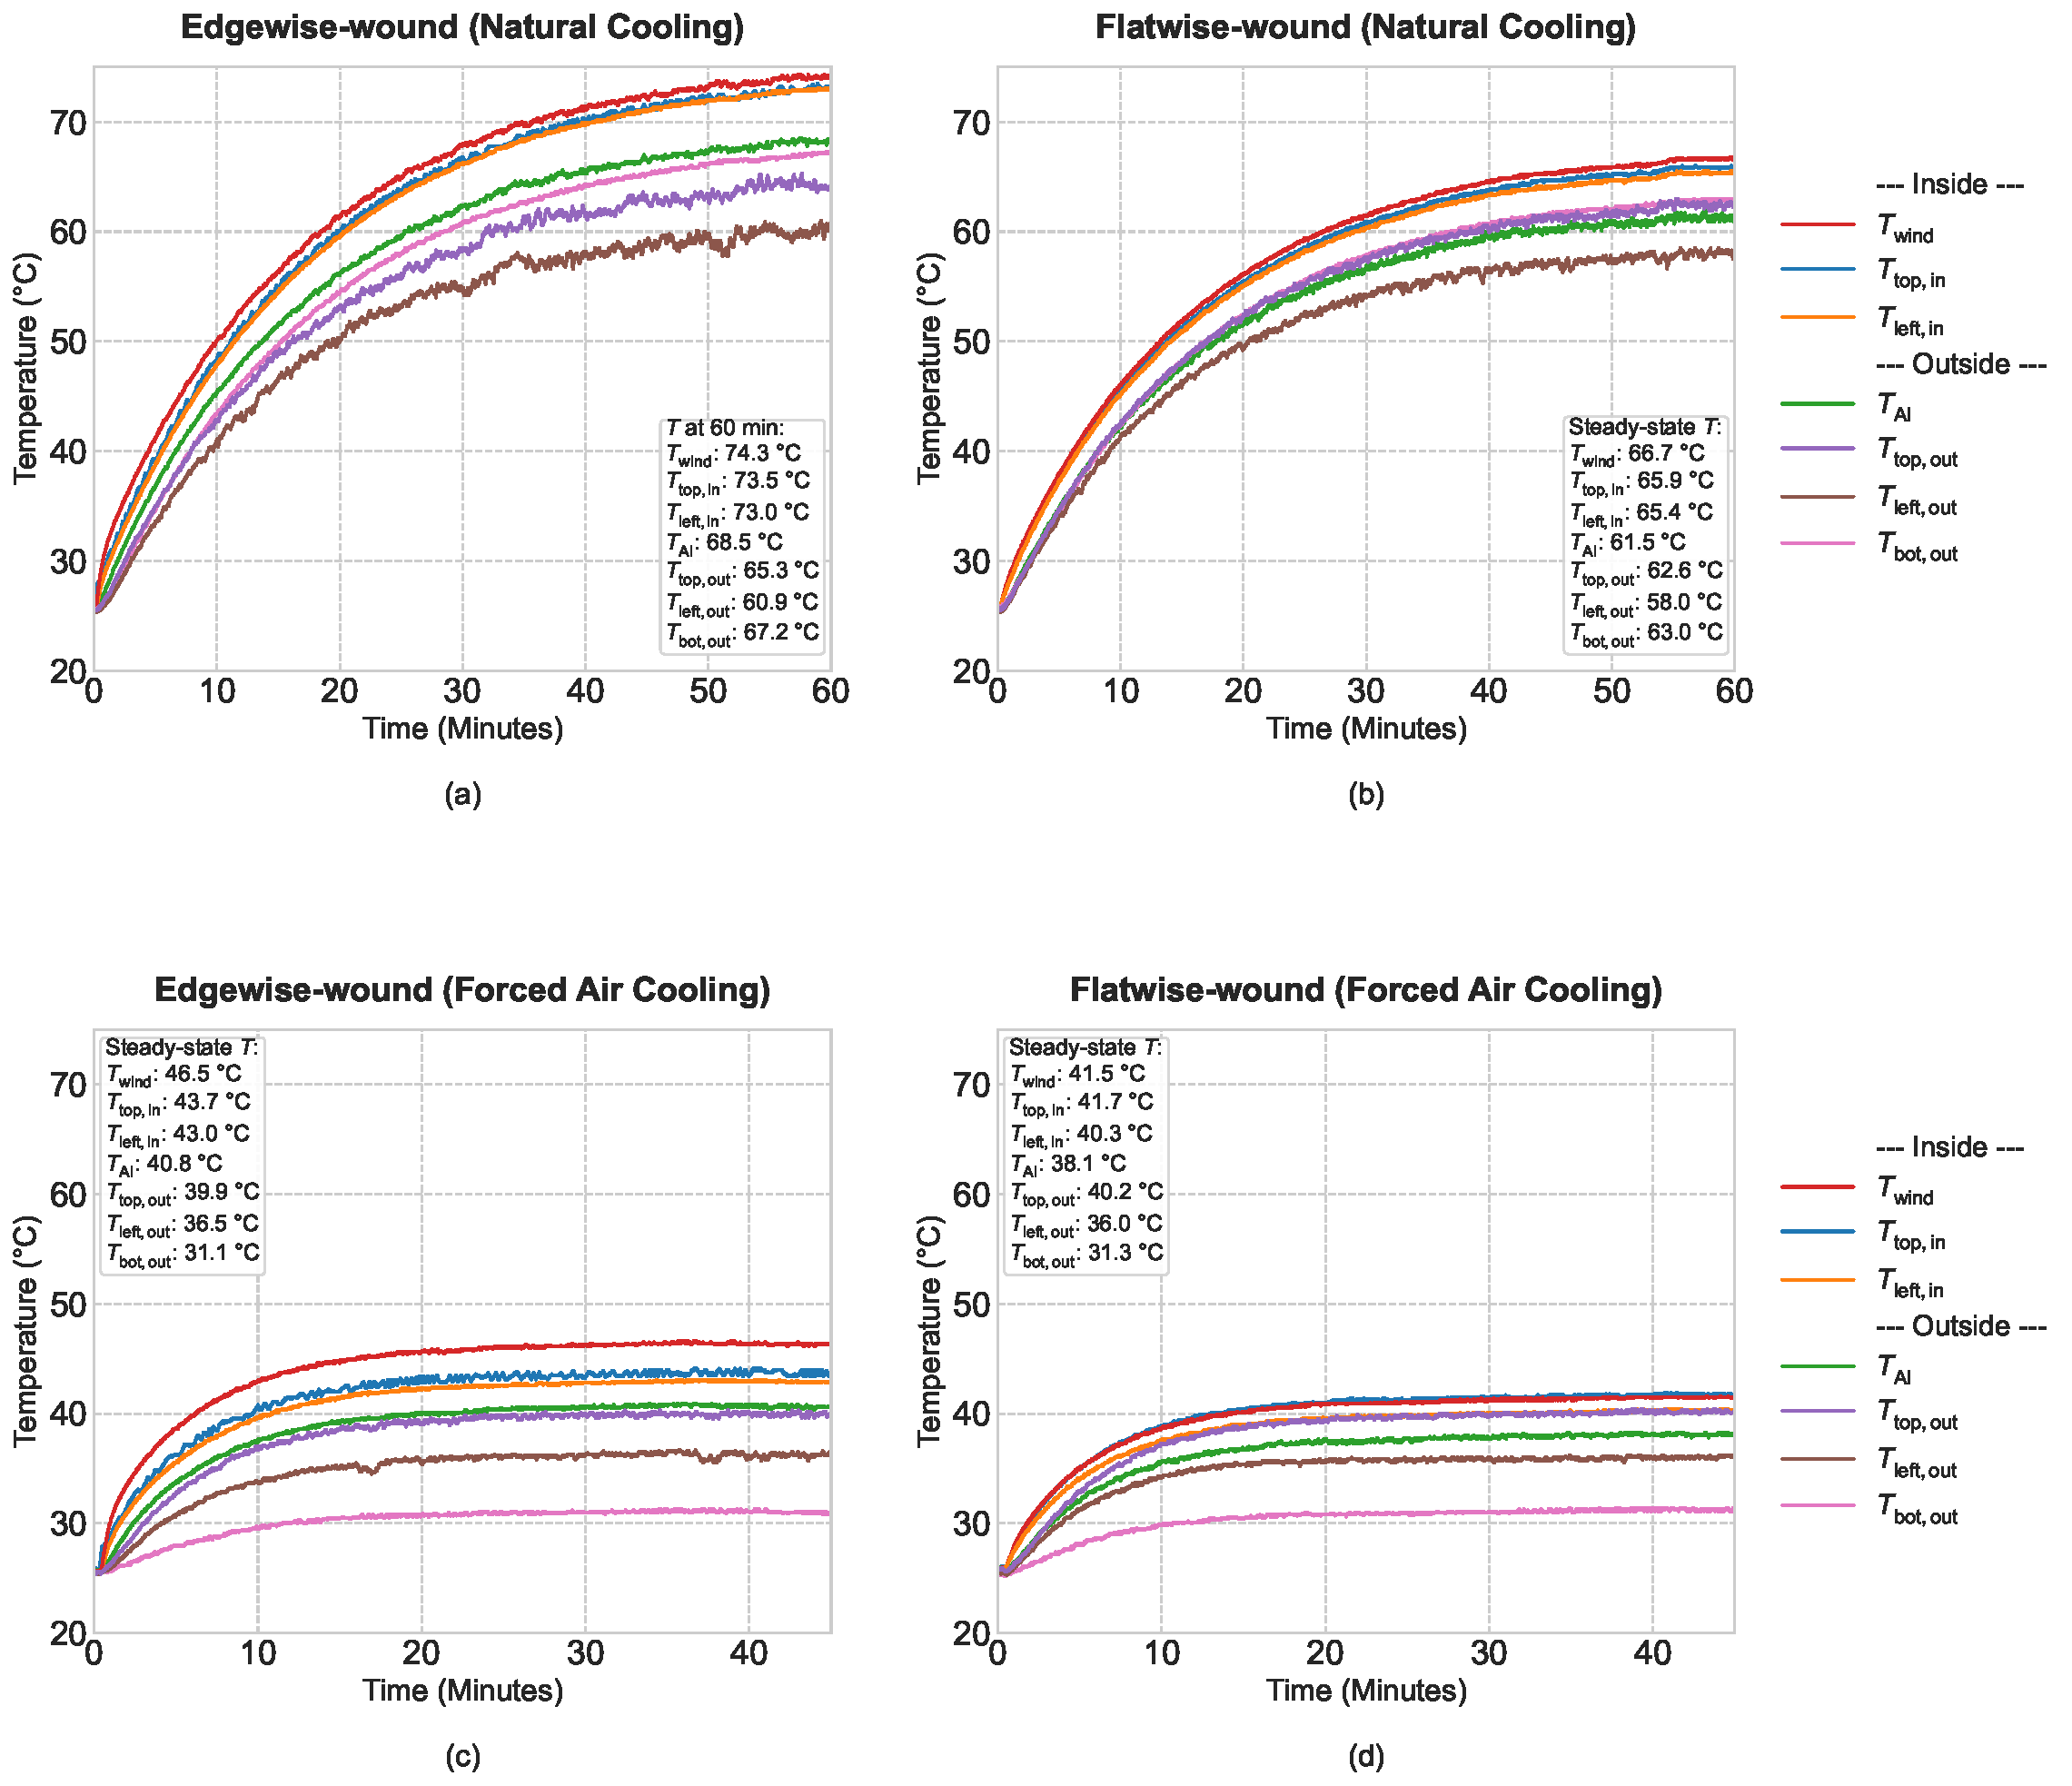
\includegraphics[width=\columnwidth]{figures_chapter5/Combined_Thermal_Comparison.pdf} 
        \caption{Temperature profiles of the transformers at natural cooling: (a) edgewise-wound transformer, (b) flatwise-wound transformer; and forced-air cooling through a heat sink: (c) edgewise-wound transformer, (d) flatwise-wound transformer.}
        \label{fig:18}
\end{figure}

%To confirm the uniformity of distribution on the surfaces of the transformer and for repeatability, the test was repeated once again. Results are shown in Figure xx.

\pagebreak
\subsection{System Efficiency}
The system-level efficiency was examined using the same 1-kW converter for each test case. An input power-efficiency curve is shown in Figure \ref{fig:eff}. The peak efficiency was observed at around 30\% or 300 W load in both cases. The full load efficiency of the system is at 92.5\%. This entails that both transformers allow for close performance, entailing no problem in using the proposed transformer. The flatwise-wound transformer is then able to guarantee superior internal-to-external thermal resistance without affecting the system-level efficiency.
\begin{figure}[h!]
\centering
% (a) Left circuit
        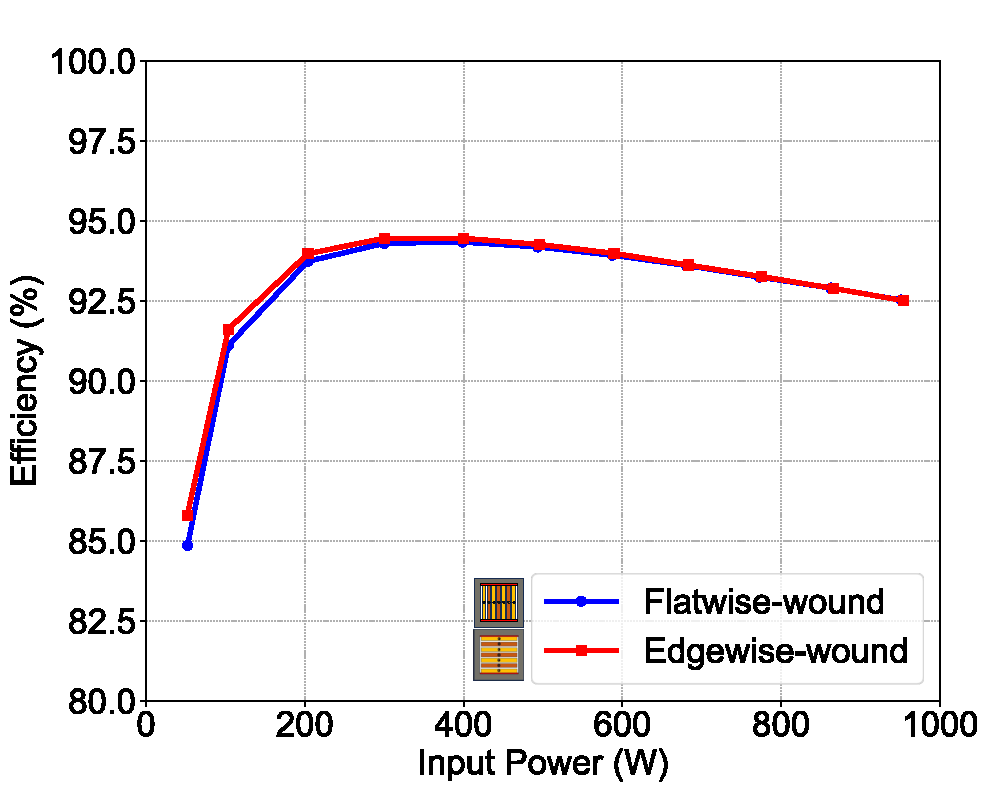
\includegraphics[width=0.7\columnwidth]{figures_chapter5/efficiency.pdf} 
        \caption{System-level efficiency of the 1-kW CLLC at 28.5 kHz operating frequency, from 50W to 1000W input power.}
        \label{fig:eff}
\end{figure}

%\subsection{Reverse Engineering Simulation}
%The simulation for the constructed prototypes were repeated once again. This time, the whole cooling setup is reproduced as close as possible in simulation. A sample of the simulation model is shown in Figure xx. 

%The 

\chapter{Scalability Analysis}
Chapters 4 and 5 demonstrated the feasibility and thermal advantages of implementing the proposed flatwise-wound transformer in a small-scale, 1~kW prototype through both finite element simulations and experimental evaluations. As theorized in Chapter 3 and validated in the preceding chapters, the flatwise winding orientation establishes parallel thermal conduction paths that significantly lower the intrinsic thermal resistance of the transformer compared to conventional edgewise windings. To further evaluate the practical viability of the proposed architecture for broader  applications, this chapter explores the scalability of the flatwise-wound transformer in terms of the benefit it can provide compared to its conventional counterpart.

Specifically, this scalability analysis is divided into two main investigations:
\begin{enumerate}
    \item \textbf{Geometric Scalability:} Evaluating the spatial effect of varying the core window aspect ratio (from low-profile to high-profile geometries) on the electromagnetic and thermal performance while maintaining a constant magnetic flux density $B_{\mathrm{m}}$, current density $J$ and magnetizing inductance $L_{\mathrm{m}}$.
    \item \textbf{Power Scalability:} Evaluating the suitability of the proposed winding structure as the operating power is scaled from 1~kW up to 10~kW and 100~kW using the Area-Product ($AP$) sizing method, while maintaining constant magnetic flux density $B_{\mathrm{m}}$, current density $J$, window occupancy ratio $K_\mathrm{u}$, and magnetizing inductance $L_{\mathrm{m}}$
\end{enumerate}
Once the scalability potential of the flatwise-wound transformer is established in these two aspects, then theoretically any kind of geometry would be feasible for the flatwise-wound transformer, allowing for 
\section{Geometric Scalability}
Having established the fundamental thermal superiority of the flatwise configuration in the square-window baseline, the simulation analysis in Chapter 4 is extended here to evaluate the impact of spatial geometry across different core window aspect ratios.

Having established the fundamental thermal superiority of the flatwise configuration in the square-window baseline, the analysis is now extended to evaluate the impact of spatial geometry across different core window aspect ratios.

To conduct this parametric sweep, two additional transformer profiles were designed for both the flatwise and edgewise configurations by varying the winding thickness $w_\mathrm{wire}$, which we will denote as $t$ from now on for brevity. This generated a spectrum of designs ranging from high-profile to low-profile models. The baseline square models are denoted as Tr2E and Tr2F. The high-profile models, denoted as Tr3E and Tr3F, utilize $t$ of 0.50 mm and 0.20 mm, respectively. Conversely, the low-profile models, denoted as Tr1E and Tr1F, utilize $t$ of 0.20 mm and 0.50 mm, respectively. The finalized parameters for the extended parametric sweep are detailed in Table \ref{tab:extended_parameters}. The new set of transformers had key parameters $L_{\mathrm{m}}$, $N_{\mathrm{p}}$ and $J$ the same as Tr2E and Tr2F. The $A_{\mathrm{win}}$ was maintained equal for each corresponding pair of edgewise and flatwise designs that share the same conductor dimensions.

\begin{table}[h]
\centering
\caption{Parameters of the Extended Transformer Aspect Ratio Models}
\label{tab:extended_parameters}
\resizebox{\textwidth}{!}{
\begin{tabular}{lcccc}
\hline
\hline
\textbf{Model}& \textbf{Wire Thickness} & \textbf{Window Area} & \textbf{Aspect Ratio} & \textbf{Dimensions} \\
 & $t$ (mm) & $A_{\mathrm{win}}$ ($\mathrm{mm}^2$) & $l_{\mathrm{win}}/w_{\mathrm{win}}$ & $l_{\mathrm{tr}} \times w_{\mathrm{tr}} \times h_{\mathrm{tr}}$ (mm) \\
\hline
Tr. 1F & 0.50 & 69.00 & 0.52 & 74.12 $\times$ 43.00 $\times$ 16.00 \\
Tr. 2F & 0.30 & 71.96 & $\sim$1.00 & 67.46 $\times$ 36.60 $\times$ 18.67 \\
Tr. 3F & 0.20 & 80.40 & 1.79 & 64.35 $\times$ 33.40 $\times$ 22.00 \\
\hline
Tr. 1E & 0.20 & 80.40 & 0.56 & 74.59 $\times$ 44.00 $\times$ 16.70 \\
Tr. 2E & 0.30 & 71.96 & $\sim$1.00 & 68.19 $\times$ 37.33 $\times$ 18.30 \\
Tr. 3E & 0.50 & 69.00 & 1.92 & 62.10 $\times$ 32.00 $\times$ 21.50 \\
\hline
\hline
\end{tabular}%
}
\end{table}

The evaluation of this parametric sweep across the three distinct aspect ratios reveals crucial insights into the geometric scalability of both winding architectures as shown in the compilation of results in Figure \ref{fig:compilation}. A summary of the peak temperatures are shown in Figure \ref{fig:summary}. The losses at each geometry are tabulated in Table \ref{tab:transformer_losses}. The edgewise-wound transformers still confirm the existence of a severe thermal bottleneck, as shown in Figure \ref{fig:compilation}a.  As the transformer profile increases, the series thermal path traps heat internally, causing the peak temperature to rise from 61.6$^\circ$C to 70.9$^\circ$C. Conversely, under natural cooling, the flatwise-wound transformers continue to exhibit excellent thermal stability as shown in Figure \ref{fig:compilation}b, maintaining a consistent peak temperature of approximately 56.0$^\circ$C and uniform heat distribution across all evaluated geometries.  

\begin{figure}[h!]
    \centering
    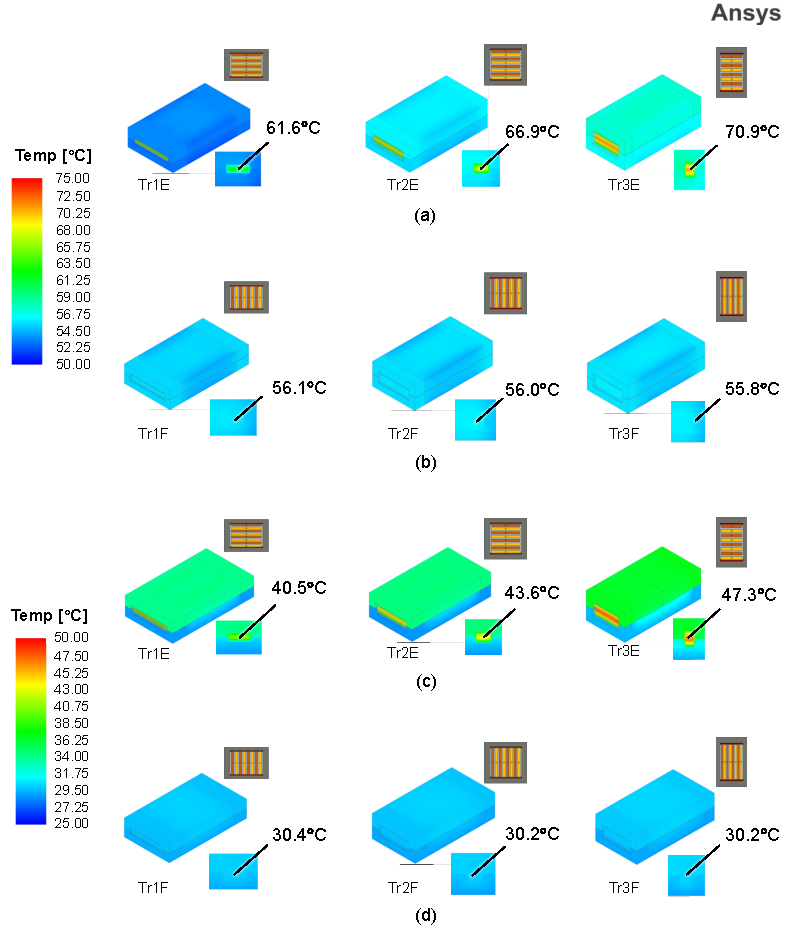
\includegraphics[width=\columnwidth]{figures_chapter4/compilation.pdf}%
    \caption{Simulated thermal distribution of the evaluated transformer models at 28.5 kHz and 25°C ambient temperature: (a) edgewise and (b) flatwise (proposed) configurations under natural cooling; (c) edgewise and (d) flatwise (proposed) configurations under forced-air cooling.}
    \label{fig:compilation}
\end{figure}

\begin{figure}[h!]
    \centering
    \subfloat[]{
        \centering
        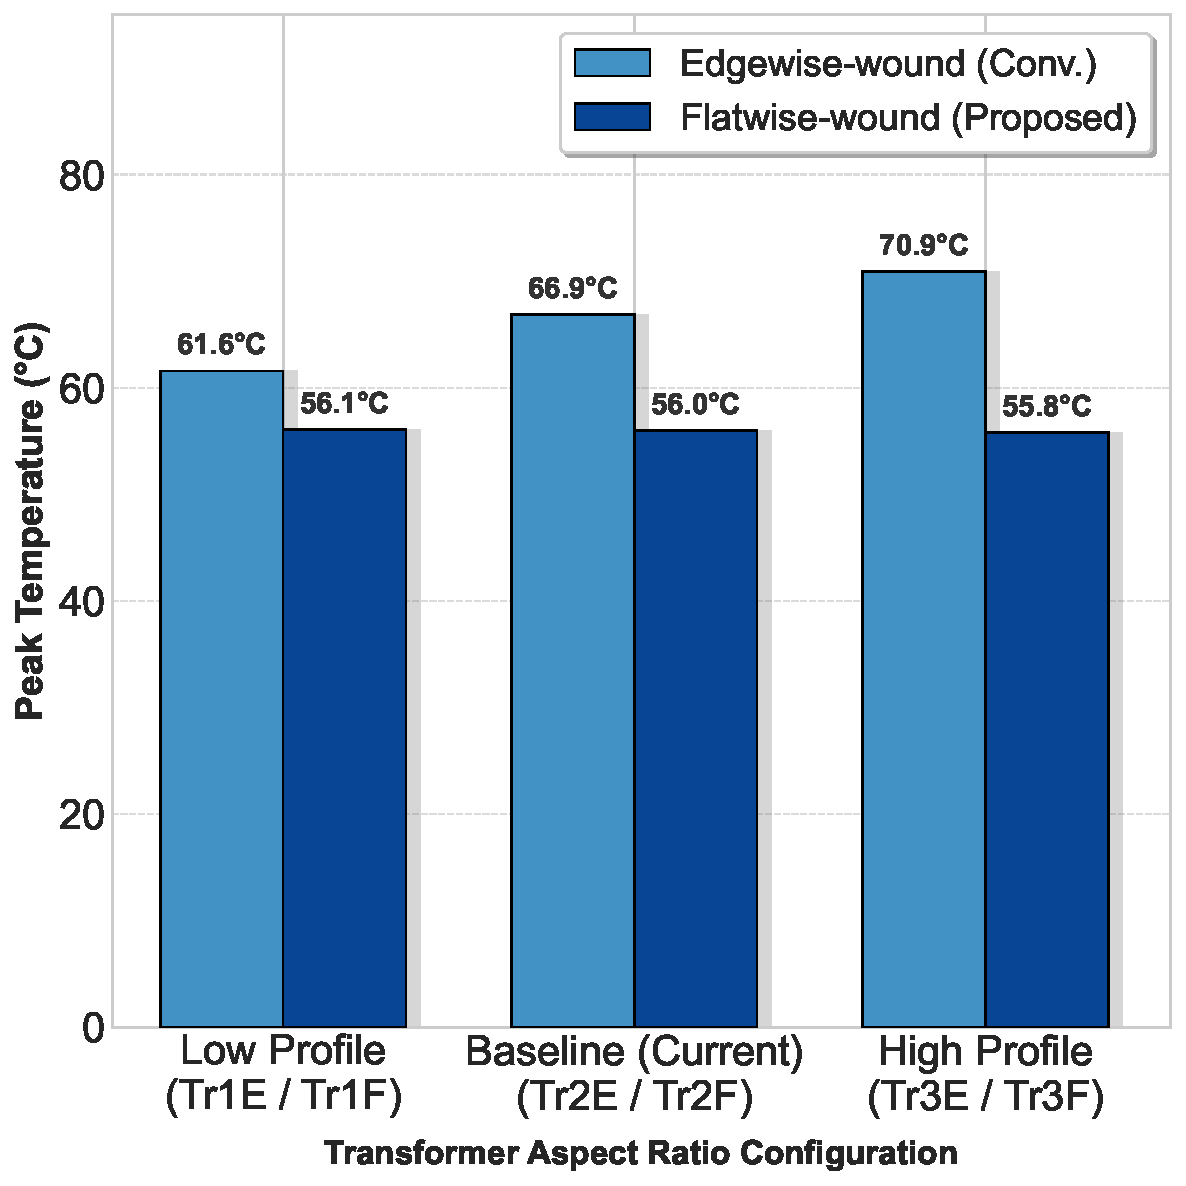
\includegraphics[width=0.45\columnwidth]{figures_chapter4/thermal_natural_grouped.pdf}
        \label{fig:compilation_natural}
    }
    \hfill
    \subfloat[]{
        \centering
        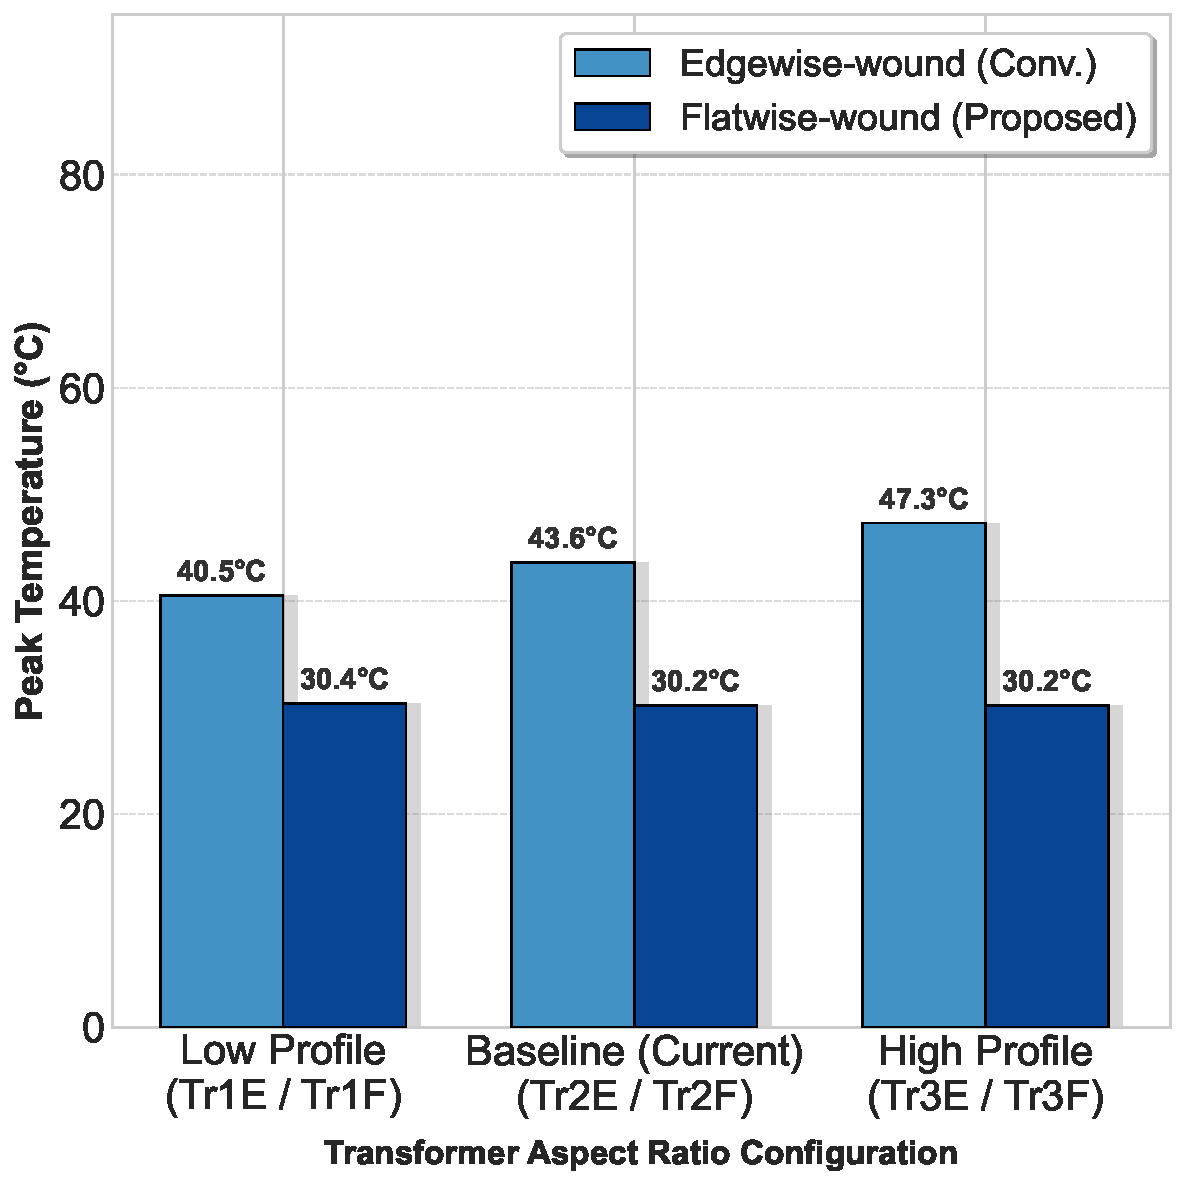
\includegraphics[width=0.45\columnwidth]{figures_chapter4/thermal_forced_grouped.pdf}
        \label{fig:compilation_forced}
    }
    \caption{Summary of peak temperatures of the evaluated transformer models at 28.5 kHz and 25°C ambient temperature: (a) edgewise and flatwise configurations under natural cooling; (b) edgewise and flatwise configurations under forced-air cooling.}
    \label{fig:summary}
\end{figure}

\begin{table}[h!]
\centering
\caption{Transformer Losses at Different Geometries}
\label{tab:transformer_losses}
% Reduces the horizontal white space between columns
% Standard IEEE table font size
\begin{tabular}{lcccccc}
\hline
\hline
\textbf{Loss} & \textbf{Tr1F} & \textbf{Tr2F} & \textbf{Tr3F} & \textbf{Tr1E} & \textbf{Tr2E} & \textbf{Tr3E} \\
\hline
Winding Losses (W)  & 2.5530 & 2.3270 & 2.2900 & 2.3990 & 2.2440 & 2.1620 \\
Core Losses (W)     & 0.8798 & 0.8715 & 0.8938 & 0.9316 & 0.8740 & 0.8900 \\
Aluminum Losses (W) & 0.1172 & 0.0902 & 0.0821 & 0.0916 & 0.0885 & 0.0874 \\
\hline
\textbf{Total Losses} (W)    & 3.5499 & 3.2891 & 3.2662 & 3.4219 & 3.2069 & 3.1395 \\
\hline
\hline
\end{tabular} 
\end{table}

The forced-air cooling scenario further confirmed this advantage. The edgewise models in Figure \ref{fig:compilation}c still exhibited heat being trapped in the windings, resulting in peaks of 40.5$^\circ$C to 47.3$^\circ$C. Moreover, as seen in Figure \ref{fig:compilation}d, the flatwise models again exhibited consistent performance, maintaining a low peak temperature of approximately 30.2$^\circ$C and a uniform temperature distribution. 

Ultimately, this comprehensive set of results highlights the profound thermal scalability of the flatwise geometry. In terms of electrical performance, the total power losses of both configurations remain practically equivalent. Noticeably, there is a spatial trade-off, as the radial stacking of the flatwise configuration inherently consumes more horizontal window space as the profile goes lower, which tends to increase the mean turn length (MTL). However, by fundamentally minimizing the internal series thermal resistance, the structure guarantees exceptional heat extraction even when integrated with practical, external cooling methods. This massive thermal headroom not only prevents localized hotspots but also unlocks the potential for further volumetric miniaturization of the transformer in high-power-density converter applications.

\section{Power Scalability}
While the 1~kW prototype and geometric sweep validate the fundamental heat extraction mechanism of the flatwise winding structure, High-Frequency Transformers (HFTs) deployed in modular SSTs and high-power DC--DC converters typically operate at tens to hundreds of kilowatts. Therefore, a power scalability analysis is conducted to evaluate the electromagnetic and thermal performance of the proposed transformer architecture as the rated power is scaled from 1~kW to 10~kW and 100~kW.

\subsection{Electrical Specifications and Scaling Assumptions}
To perform a rigorous and fair comparison across different power levels, the electrical parameters of the CLLC resonant converter are scaled such that the underlying circuit dynamics and resonant tank characteristics remain consistent. Specifically, as the output power $P_{\mathrm{o}}$ is increased by a factor of 10 (to 10~kW) and 100 (to 100~kW), both the input and output voltages $V_{\mathrm{in}}, V_{\mathrm{o}}$ and the input and output currents $I_{\mathrm{in}}, I_{\mathrm{o}}$ are scaled equally. 

By scaling voltage and current at the same rate as had been explained in Chapter \ref{sec:established}, the effective load resistance $R_{\mathrm{o}} = V_{\mathrm{o}}/I_{\mathrm{o}}$ and the equivalent AC resistance derived via First Harmonic Approximation (FHA) given by Eq. \ref{eq:Rac}
remain constant across all power levels. Consequently, the quality factor $Q$, inductance ratio $k = 10.0$, voltage gain curve $M$, and resonant tank components $C_{\mathrm{r1}} = C_{\mathrm{r2}} = 1.4~\mu\text{F}$, $L_{\mathrm{r1}} = L_{\mathrm{r2}} = 20.1~\mu\text{H}$, and $L_{\mathrm{m}} = 200~\mu\text{H}$ remain identical for the 1~kW, 10~kW, and 100~kW designs. The electrical specifications across the three power ratings are summarized in Table~\ref{tab:power_electrical_specs}. More insight behind this choice of parameters is explained in Chapter \ref{sec:established}. 

\begin{table}[h!]
\centering
\caption{Electrical Specifications for the Power Scalability Analysis}
\label{tab:power_electrical_specs}
\begin{tabular}{llccc}
\hline
\hline
\textbf{Parameter} & \textbf{Symbol} & \textbf{1 kW} & \textbf{10 kW} & \textbf{100 kW} \\
\hline
Input Voltage & $V_{\mathrm{in}}$ & 100 V & $316\text{ V } (\times\sqrt{10})$ & $1000\text{ V } (\times 10)$ \\
Output Voltage & $V_{\mathrm{o}}$ & 100 V & $316\text{ V } (\times\sqrt{10})$ & $1000\text{ V } (\times 10)$ \\
Output Current & $I_{\mathrm{o}}$ & 10 A & $31.6\text{ A } (\times\sqrt{10})$ & $100\text{ A } (\times 10)$ \\
Output Power & $P_{\mathrm{o}}$ & 1 kW & $10\text{ kW } (\times 10)$ & $100\text{ kW } (\times 100)$ \\
Switching Frequency & $f_{\mathrm{sw}}$ & 28.5 kHz & 28.5 kHz & 28.5 kHz \\
Resonant Frequency & $f_{\mathrm{r}}$ & 30.0 kHz & 30.0 kHz & 30.0 kHz \\
Dead Time & $t_{\mathrm{d}}$ & 360 ns & 360 ns & 360 ns \\
Resonant Capacitance & $C_{\mathrm{r1}}, C_{\mathrm{r2}}$ & $1.4~\mu\text{F}$ & $1.4~\mu\text{F}$ & $1.4~\mu\text{F}$ \\
Resonant Inductance & $L_{\mathrm{r1}}, L_{\mathrm{r2}}$ & $20.1~\mu\text{H}$ & $20.1~\mu\text{H}$ & $20.1~\mu\text{H}$ \\
Target Mag. Inductance & $L_{\mathrm{m}}$ & $200~\mu\text{H}$ & $200~\mu\text{H}$ & $200~\mu\text{H}$ \\
\hline
\hline
\end{tabular}
\end{table}

\subsection{Area-Product ($AP$) Sizing Guidelines}
To scale the physical geometry of the baseline square-window transformers (Tr2E and Tr2F, denoted here as Tr.~E-1 and Tr.~F-1) to 10~kW (Tr.~E-10 and Tr.~F-10) and 100~kW (Tr.~E-100 and Tr.~F-100), the Area-Product ($AP$) method is utilized[cite: 47, 53, 58]. The area product relates the physical window area $A_{\mathrm{w}}$ and magnetic core cross-sectional area $A_{\mathrm{c}}$ to the electrical and magnetic constraints of the converter[cite: 53, 54]:
\begin{equation}
    AP = A_{\mathrm{w}} \cdot A_{\mathrm{c}} = \frac{V_{\mathrm{in}}(I_{\mathrm{p,rms}} + I_{\mathrm{s,rms}})}{K_{\mathrm{f}} f_{\mathrm{sw}} B_{\mathrm{m}} J_{\mathrm{m}} K_{\mathrm{u}}} = \frac{2 P_{\mathrm{o}}}{4 f_{\mathrm{sw}} B_{\mathrm{m}} J_{\mathrm{m}} K_{\mathrm{u}}},
\end{equation}
where $K_{\mathrm{f}} = 4$ is the waveform coefficient for square-wave voltage excitation ($n = 1$, $D = 0.5$), $B_{\mathrm{m}}$ is the maximum core flux density, $J_{\mathrm{m}}$ is the current density, and $K_{\mathrm{u}}$ is the window utilization factor[cite: 53, 69, 70]. 

In this scaling procedure, $L_{\mathrm{m}}$, $B_{\mathrm{m}}$, $J_{\mathrm{m}}$, $K_{\mathrm{u}}$, and the number of turns $N_{\mathrm{p}}:N_{\mathrm{s}} = 8:8$ are held constant across all power levels[cite: 52, 55, 58]. Separating the area product into its constituent components yields[cite: 54]:
\begin{equation}
    A_{\mathrm{c}} \ge \frac{V_{\mathrm{in}}}{4 f_{\mathrm{sw}} N_{\mathrm{p}} B_{\mathrm{m}}}, \quad A_{\mathrm{w}} = \frac{N_{\mathrm{p}}(I_{\mathrm{p,rms}} + I_{\mathrm{s,rms}})}{J_{\mathrm{m}} K_{\mathrm{u}}}.
\end{equation}
Thus, the core cross-sectional area $A_{\mathrm{c}}$ is proportional to the operating voltage ($A_{\mathrm{c}} \propto V_{\mathrm{in}}$), whereas the window area $A_{\mathrm{w}}$ is proportional to the operating current ($A_{\mathrm{w}} \propto I$)[cite: 54]. Let $\lambda_V$ and $\lambda_I$ represent the one-dimensional (1D) linear scaling factors for the core and window dimensions, respectively[cite: 54]:
\begin{equation}
    A_{\mathrm{c,new}} = (\lambda_V w_{\mathrm{core,old}})(\lambda_V l_{\mathrm{core,old}}) = \lambda_V^2 A_{\mathrm{c,old}} \implies \lambda_V = \sqrt{\frac{V_{\mathrm{new}}}{V_{\mathrm{old}}}},
\end{equation}
\begin{equation}
    A_{\mathrm{w,new}} = (\lambda_I w_{\mathrm{win,old}})(\lambda_I l_{\mathrm{win,old}}) = \lambda_I^2 A_{\mathrm{w,old}} \implies \lambda_I = \sqrt{\frac{I_{\mathrm{new}}}{I_{\mathrm{old}}}}.
\end{equation}

Because voltage and current are scaled equally ($V_{\mathrm{new}}/V_{\mathrm{old}} = I_{\mathrm{new}}/I_{\mathrm{old}}$), the 1D scaling factors are identical ($\lambda_V = \lambda_I$), which preserves the square window aspect ratio ($l_{\mathrm{win}}/w_{\mathrm{win}} \approx 1.00$) and constant window utilization factor $K_{\mathrm{u}}$ across all power levels[cite: 51, 52, 55, 58]:
\begin{itemize}
    \item \textbf{Core Dimensions:} The center-leg ($l_{\mathrm{core}} \times w_{\mathrm{core}}$) and outer-leg ($l_{\mathrm{core}} \times 0.5w_{\mathrm{core}}$) dimensions are scaled linearly by $\lambda_V$[cite: 55, 56, 57].
    \item \textbf{Window and Conductor Dimensions:} The window width $w_{\mathrm{win}}$, window height $l_{\mathrm{win}}$, wire thickness $t$, clearances $d_{\mathrm{clear}}$, TIM thickness $d_{\mathrm{TIM}}$, and inter-turn insulation distance $d_{\mathrm{inter}}$ are scaled linearly by $\lambda_I$[cite: 52, 55, 56, 57].
    \item \textbf{Air Gap Length:} To maintain a constant magnetizing inductance $L_{\mathrm{m}} \approx \mu_0 N_{\mathrm{p}}^2 A_{\mathrm{c}} / l_{\mathrm{g}}$ as $A_{\mathrm{c}}$ increases by $\lambda_V^2$, the air gap length $l_{\mathrm{g}}$ is scaled proportionally to the voltage ratio ($\lambda_V^2$)[cite: 52, 55]:
    \begin{equation}
        l_{\mathrm{g,new}} = l_{\mathrm{g,old}} \frac{A_{\mathrm{c,new}}}{A_{\mathrm{c,old}}} = \lambda_V^2 l_{\mathrm{g,old}}.
    \end{equation}
\end{itemize}

The total area-product scaling factor is defined as $\lambda_{AP} = \lambda_V \cdot \lambda_I$[cite: 55]. Since transformer volume scales according to $Vol_{\mathrm{tr}} \propto P_{\mathrm{o}}^{3/4} \propto AP^{3/4}$, the overall three-dimensional volume of the scaled transformers increases by $\lambda_{AP}^{3/4}$[cite: 62, 69]. The resulting physical and electrical parameters for the 1~kW, 10~kW, and 100~kW transformer models are detailed in Table~\ref{tab:power_scaling_specs}[cite: 58, 62].

\begin{table}[h!]
\centering
\caption{Simulation Specifications and Dimensions for the Power Scalability Models[cite: 58, 62]}
\label{tab:power_scaling_specs}
\resizebox{\textwidth}{!}{%
\begin{tabular}{lcccccc}
\hline
\hline
\textbf{Parameter} & \textbf{Tr. F-1} & \textbf{Tr. F-10} & \textbf{Tr. F-100} & \textbf{Tr. E-1} & \textbf{Tr. E-10} & \textbf{Tr. E-100} \\
\hline
Rated Power $P_{\mathrm{o}}$ & 1 kW & 10 kW & 100 kW & 1 kW & 10 kW & 100 kW \\
Voltage Scaling Factor $\lambda_V$ & 1 & $\sqrt[4]{10}$ & $\sqrt{10}$ & 1 & $\sqrt[4]{10}$ & $\sqrt{10}$ \\
Current Scaling Factor $\lambda_I$ & 1 & $\sqrt[4]{10}$ & $\sqrt{10}$ & 1 & $\sqrt[4]{10}$ & $\sqrt{10}$ \\
$AP$ Scaling Factor $\lambda_{AP}$ & 1 & $\sqrt{10}$ & 10 & 1 & $\sqrt{10}$ & 10 \\
Wire Thickness $t$ (mm) & 0.30 & 0.53 & 0.95 & 0.30 & 0.53 & 0.95 \\
Aspect Ratio $l_{\mathrm{win}}/w_{\mathrm{win}}$ & $\sim$1.00 & $\sim$1.00 & $\sim$1.00 & $\sim$1.00 & $\sim$1.00 & $\sim$1.00 \\
Air Gap $l_{\mathrm{g}}$ (mm) & 0.10 & 0.32 & 1.00 & 0.10 & 0.32 & 1.00 \\
Mag. Inductance $L_{\mathrm{m}}$ ($\mu$H) & 200.00 & 208.11 & 216.49 & 200.00 & 207.36 & 215.24 \\
Dimensions $l_{\mathrm{tr}} \times w_{\mathrm{tr}} \times h_{\mathrm{tr}}$ (mm) & \makecell{67.46 $\times$ 36.60 \\ $\times$ 18.67} & \makecell{119.96 $\times$ 65.09 \\ $\times$ 33.20} & \makecell{213.33 $\times$ 115.74 \\ $\times$ 59.03} & \makecell{68.19 $\times$ 37.33 \\ $\times$ 18.30} & \makecell{121.27 $\times$ 66.39 \\ $\times$ 32.54} & \makecell{215.65 $\times$ 118.06 \\ $\times$ 57.87} \\
\hline
\hline
\end{tabular}%
}
\end{table}

\subsection{Electromagnetic-Thermal Simulation Results}
To provide a standardized, general representation of active cooling across all three power scales, each transformer is mounted via a bottom TIM layer onto a fixed $20^\circ\text{C}$ cold-plate boundary covering the bottom surface of the transformer, with the surrounding ambient air at $25^\circ\text{C}$[cite: 52, 59, 60, 61]. This boundary condition ensures that the cooling capability scales proportionally with the bottom footprint area of each transformer, guaranteeing a fair comparison between the edgewise and flatwise structures[cite: 52, 62].

The simulated temperature distributions for the 1~kW, 10~kW, and 100~kW models are illustrated in Figure~\ref{fig:power_thermal_dist}[cite: 59, 60, 61, 88, 89, 90], while the comparative summaries of peak winding temperatures and loss breakdowns are presented in Figure~\ref{fig:power_scalability_summary} and Table~\ref{tab:power_scaling_losses}[cite: 63, 88, 89, 90].


\begin{table}[h!]
\centering
\caption{Simulated Losses and Peak Winding Temperatures Across Scaled Power Ratings[cite: 59, 60, 61, 63, 88, 89, 90]}
\label{tab:power_scaling_losses}
\resizebox{\textwidth}{!}{%
\begin{tabular}{lcccccc}
\hline
\hline
\textbf{Metric} & \textbf{Tr. F-1} & \textbf{Tr. F-10} & \textbf{Tr. F-100} & \textbf{Tr. E-1} & \textbf{Tr. E-10} & \textbf{Tr. E-100} \\
\hline
Winding Losses $P_{\mathrm{wind}}$ (W) & 2.33 & 15.09 & 126.40 & 2.24 & 14.50 & 107.90 \\
Core Losses $P_{\mathrm{core}}$ (W) & 0.87 & 4.91 & 27.27 & 0.87 & 4.95 & 27.66 \\
Aluminum Losses $P_{\mathrm{Al}}$ (W) & 0.09 & 1.39 & 12.66 & 0.09 & 1.38 & 13.10 \\
\hline
\textbf{Total Losses (W)} & \textbf{3.29} & \textbf{21.39} & \textbf{166.33} & \textbf{3.21} & \textbf{20.83} & \textbf{148.66} \\
\hline
\textbf{Peak Winding Temp. ($^\circ$C)} & \textbf{21.2} & \textbf{24.2} & \textbf{37.0} & \textbf{36.8} & \textbf{78.2} & \textbf{210.6} \\
\hline
\hline
\end{tabular}%
}
\end{table}

As demonstrated in Table~\ref{tab:power_scaling_losses} and Figure~\ref{fig:power_scalability_summary}(a), the divergence in thermal performance between the two winding orientations becomes dramatically amplified as the power rating increases[cite: 63]:
\begin{itemize}
    \item \textbf{At 1~kW:} With the $20^\circ\text{C}$ bottom cold plate, the conventional edgewise transformer (Tr.~E-1) reaches a peak winding temperature of $36.8^\circ\text{C}$, whereas the proposed flatwise transformer (Tr.~F-1) remains at just $21.2^\circ\text{C}$ (only $1.2^\circ\text{C}$ above the cold-plate temperature)[cite: 52, 59, 88].
    \item \textbf{At 10~kW:} As total losses increase to approximately 21~W and the inter-turn insulation layers scale thicker by $\lambda_I = \sqrt[4]{10}$, the series thermal resistance of the edgewise winding traps heat in the upper turns, driving the peak temperature of Tr.~E-10 to $78.2^\circ\text{C}$[cite: 25, 56, 58, 60]. In stark contrast, the parallel heat conduction paths of the flatwise design (Tr.~F-10) restrict the peak winding temperature to $24.2^\circ\text{C}$[cite: 23, 60, 89].
    \item \textbf{At 100~kW:} At full SST module scale, the conventional edgewise design (Tr.~E-100) experiences severe thermal runaway, reaching an unsustainable peak winding temperature of $210.6^\circ\text{C}$ due to the cumulative thermal resistance of the stacked insulation layers and the increased vertical distance from the bottom cold plate[cite: 25, 52, 56, 61]. Conversely, the proposed flatwise-wound transformer (Tr.~F-100) maintains a remarkable peak winding temperature of only $37.0^\circ\text{C}$[cite: 61, 90].
\end{itemize}

Examining the loss breakdown in Figure~\ref{fig:power_scalability_summary}(b) and Table~\ref{tab:power_scaling_losses}, the flatwise configuration incurs a slightly higher AC winding loss at 100~kW ($126.40\text{ W}$ vs.\ $107.90\text{ W}$ for edgewise), resulting in a total loss of $166.33\text{ W}$ compared to $148.66\text{ W}$[cite: 63, 90]. This marginal increase (representing only a $0.018\%$ difference in overall efficiency at 100~kW) occurs because the conductor thickness scales to $t = 0.95\text{ mm}$ at 100~kW—approaching the skin depth limit at 28.5~kHz—and the vertical orientation of the flatwise turns experiences slightly higher fringing flux near the air gap[cite: 23, 27, 57, 58]. Nevertheless, delivering a $173.6^\circ\text{C}$ reduction in peak winding temperature at 100~kW in exchange for a negligible increase in conduction loss proves that the proposed flatwise-wound architecture is exceptionally well-suited for high-power, high-density SST applications[cite: 5, 61, 63].


\chapter{Summary and Conclusion}
\section{Summary and Conclusion}
This thesis presented the comprehensive design, comparative analysis, and experimental validation of a flatwise-wound planar transformer engineered to resolve the fundamental thermal bottlenecks in high-power-density Solid State Transformers (SSTs). Traditional planar transformers predominantly utilize an edgewise winding architecture, which inherently traps heat due to the high series thermal resistance of the inter-turn dielectric insulation. To overcome this critical limitation, this study proposed a structural shift to a flatwise orientation, establishing a highly conductive parallel thermal path that grants every individual copper turn direct, orthogonal access to the external cooling boundaries.

The theoretical advantages of this geometric reconfiguration were first evaluated through comprehensive 3D Multi-Physics Finite Element Analysis (FEA). Baseline simulations confirmed that the flatwise orientation inherently provides a superior thermal path by significantly lowering the peak operating temperature and eliminating localized hotspots under both natural and forced-air cooling conditions compared to the conventional edgewise equivalent. 

To definitively validate these findings, hardware prototypes of both winding configurations were fabricated and subjected to continuous, full-load experimental evaluation in a 1~kW, 28.5~kHz bidirectional CLLC resonant converter. The hardware testing conclusively validated the core hypothesis of this research. Under continuous steady-state operation, the conventional edgewise design suffered from severe internal-to-external thermal gradients, resulting in trapped heat and the rapid onset of thermal runaway. In stark contrast, the flatwise design consistently maintained safe operation, achieving significantly lower thermal gradients and reduced peak winding temperatures across all tested ambient conditions. By narrowing the temperature gradients between the internal copper windings and the core exterior, the experimental data proves that the flatwise architecture successfully establishes a fundamentally lower thermal resistance path. This enables highly efficient heat extraction directly from the core window, ultimately breaking the restrictive dielectric-thermal trade-off.

Finally, the scalability of the flatwise winding architecture was examined under controlled parameters. A geometric scalability analysis evaluated across varying core window aspect ratios at 1~kW revealed that the flatwise structure guarantees exceptional heat extraction even in high or low-profile physical geometries, establishing that the configuration is versatile in terms of spatial geometry. Furthermore, a power scalability analysis utilizing the Area-Product ($AP$) method evaluated the configurations at 10~kW and 100~kW operating limits maintaining a square window area. The results demonstrated that as the power rating and corresponding interwinding distances scale up, the thermal divergence between the two structures amplifies drastically. The flatwise-wound sturcture is able to reduce high-power peak temperatures, delivering exceptional thermal stability in exchange for only a marginal increase in total power loss at almost the same foot print with its conventional counterpart.

Ultimately, the comprehensive findings of this study validate the flatwise-wound planar transformer as a structurally superior candidate for compact, high-reliability power converters. By providing massive thermal headroom with only a marginal trade-off in high-frequency winding loss, this architecture successfully unlocks new limits for volumetric miniaturization in next-generation electrical distribution infrastructure.

\section{Recommendations and Future Work}
Building upon the established results of this study, a few key areas for recommendation and future work are suggested as follows:

\begin{itemize}
    \item \textbf{Model Verification and Optimization:} While the 3D Multi-Physics FEA provided a robust theoretical foundation for the thermal advantages of the flatwise orientation, further refinement of the analytical models is recommended. Developing faster analytical thermal and electromagnetic models will provide critical insights for design optimization, especially for larger, high-power applications where extensive 3D FEA parametric sweeps become computationally prohibitive.
    
    \item \textbf{Parasitics Modeling and Mitigation:} The proposed transformer utilizes rectangular windings. This geometry implies that parasitic capacitance will be a dominant factor, as rectangular windings feature large overlapping surface areas. A direct analogy can be drawn to PCB-based planar transformers, where large overlapping areas between adjacent copper layers inherently generate significant inter-turn and inter-winding capacitances. Future work should prioritize the development of an accurate high-frequency analytical model to extract these distributed parasitic elements. Understanding and quantifying these capacitive effects is strictly necessary to accurately predict common-mode electromagnetic interference (EMI) and mitigate unintended high-frequency ringing, which are critical steps before integrating the transformer into high-voltage, high-frequency SST applications as an example.
    
    \item \textbf{Further Scalability Analysis and High-Voltage Experimentation:} As this study successfully validated the flatwise architecture on a scaled-down 1~kW prototype, future work must formally evaluate the structural and thermal viability of this design toward the ultimate 100~kW, 1000~V target hardware. Transitioning to the 1~kV operating regime necessitates strict adherence to international safety and insulation standards, such as IEC 60664 and IEC 62477. As established in Chapter 6, future physical iterations must incorporate comprehensive insulation coordination, explicitly meeting rigorous creepage and clearance distance requirements. Experimental validation at this scale will be crucial to ensure that the physical structural modifications required for high-voltage compliance do not inadvertently compromise the established thermal advantages of the flatwise winding configuration.
\end{itemize}

\singlespacing
\phantomsection
\addcontentsline{toc}{chapter}{Research Achievements in NU PELab}
\chapter*{Research Achievements in Nagoya University Power Electronics Laboratory}
\subsection*{Journal Papers}
\begin{itemize}
    \item \textbf{K. Roque}, H. Hirasawa, S. Choi, Y. Yonezawa, J. Imaoka, and M. Yamamoto, ``Design and Implementation of a Non-coupled Integrated Transformer for a Two-phase Interleaved Flyback PFC Rectifier'', \textbf{IEEE Transactions in Industrial Applications}. \textbf{[under review]}
    \item \textbf{K. Roque}, I. Masuda, S. Choi, J. Imaoka, M. Yamamoto, M. Kauhanen, and K. Tashiro, ``Comparative Analysis of Flatwise and Edgewise Windings for Improved Thermal Management in Transformers'', \textbf{IEEJ Transactions in Industrial Applications}. \textbf{[under review]}
\end{itemize}

\subsection*{International Conferences}
\begin{itemize}
    \item \textbf{K. Roque}, I. Masuda, S. Choi, J. Imaoka, M. Yamamoto, M. Kauhanen, and K. Tashiro, ``Flatwise Windings for Improved Thermal Management in High Power Transformer Applications'', Proceedings of the \textbf{41st Applied Power Electronics Conference} (APEC) 2026, San Antonio, Texas, USA, 22-26 March 2026. \textbf{(Poster Presenter, Dialogue Preview Session Presenter)}
    
    \item \textbf{K. Roque}, I. Masuda, S. Choi, J. Imaoka, M. Yamamoto, M. Kauhanen, and K. Tashiro, ``Comparative Analysis of Flatwise and Edgewise Windings for Improved Thermal Management in Transformers'', Proceedings of the \textbf{10th International Power Electronics Conference} (IPEC - ECCE Asia) 2026, Nagasaki, Japan, May 31 -- June 04 2026. \textbf{(Poster Presenter)}
    
    \item \textbf{K. Roque}, I. Masuda, S. Choi, J. Imaoka, M. Yamamoto, M. Kauhanen, and K. Tashiro, ``An Investigation on Flatwise Windings for Improved Thermal Management in Transformers'', Proceedings of the \textbf{International Conference on Materials and Sustainability}, Nagoya University, Nagoya, Japan, 12-14 December 2025. \textbf{(Oral Presenter)}
    
    \item \textbf{K. Roque}, T. Warnakulasooriya, S. Choi, Y. Yonezawa, D. Arai, M. Yamamoto, Y. Ushida, and T. Oka, ``Theoretical Loss Analysis of Vertical GaN MOSFETs in a Totem-pole Bridgeless PFC Considering Parameter Variation'', Proceedings of the \textbf{International Conference on Materials and Sustainability}, Nagoya University, Nagoya, Japan, 1-2 December 2023. \textbf{(Oral Presenter)}
    
    \item Y. Yonezawa, \textbf{K. Roque}, and M. Yamamoto, ``Noise Simulation for Front-Loading Power Electronics EMI Design in Electric Aircraft Applications'', \textbf{SAE E-40 Electrified Propulsion Committee Workshop}, Tokyo, Japan, 17-19 March 2026. \textbf{(Oral Presenter)}
    
    \item H. Hirasawa, \textbf{K. Roque}, S. Choi, Y. Yonezawa, J. Imaoka, and M. Yamamoto, ``Design Method of an Integrated Transformer for a Two-phase Interleaved Flyback PFC Rectifier'', Proceedings of the 16th \textbf{Energy Conversion Congress and Exposition} (ECCE) 2024, Phoenix, Arizona, USA, 20-24 October 2024. \textbf{(Oral Presenter)}
\end{itemize}

\subsection*{Domestic Conferences}
\begin{itemize}
    \item \textbf{K. Roque}, T. Warnakulasooriya, S. Choi, Y. Yonezawa, D. Arai, M. Yamamoto, Y. Ushida, and T. Oka, ``Theoretical Loss Analysis of Vertical GaN MOSFETs in a Totem-pole Bridgeless PFC Considering Drift Layer Variation'', \textbf{2024 IEEJ National Convention}, 2024. \textbf{(Oral Presenter)}
    
    \item R. Borres, \textbf{K. Roque}, Y. Yonezawa, and M. Yamamoto, ``Thermal-Aware Behavioral Simulation Model Development of a 1.5 MW Converter Utilizing Vertical GaN for Electric Aircraft Applications'', \textbf{IEICE Technical Committee on Energy Engineering in Electronics and Communications}, 2026.
    
    \item H. Hirasawa, \textbf{K. Roque}, S. Choi, Y. Yonezawa, J. Imaoka, and M. Yamamoto, ``Application and Design Method of an Integrated Transformer in a Two-Phase AC-DC Interleaved Flyback Converter'', \textbf{2024 IEEJ National Convention}, 2024.
    
    \item H. Hirasawa, S. Choi, \textbf{K. Roque}, Y. Yonezawa, J. Imaoka, and M. Yamamoto, ``AC-DC Interleaved Flyback Converter with an Integrated Transformer'', \textbf{IEICE Technical Committee on Energy Engineering in Electronics and Communications}, 2023.
\end{itemize}

\subsection*{Achievements}
\begin{itemize}
    \item Dialogue Preview Session Presenter -- Top 8\% Paper in IEEE APEC 2026.
    \item G30 Automotive Engineering Program Master's Midterm Presentation -- Best Interim Presentation
\end{itemize}

\singlespacing
\printbibliography[heading=bibintoc,title={Bibliography}]
\doublespacing
% --- ADD THESE LINES TO CREATE THE TOC ENTRY ---
\clearpage
\phantomsection
\addcontentsline{toc}{chapter}{Appendices} 
% -----------------------------------------------

\appendix % <--- USE THIS ONLY ONCE!
\phantomsection
\chapter{Downsizing Effect Calculation}\label{app:downsizing}
This appendix details the theoretical derivation for the transformer downsizing effect presented in the Introduction, Figure \ref{fig:downsizing}. The volume comparison between a standard 50 Hz line-frequency transformer (LFT) and a high-frequency solid-state transformer (HFT) is evaluated using the fundamental area-product method.

\subsection*{The Area-Product Volume Equation}
The overall physical volume of a transformer ($Vol_{\mathrm{trans}}$) is proportional to the area product of its core and can be analytically estimated using the following relationship:
$$ Vol_{\mathrm{trans}} = K_{\mathrm{vol}} \left( \frac{P_{\mathrm{t}}}{K_{\mathrm{u}} \cdot B_{\mathrm{m}} \cdot f \cdot K_{\mathrm{f}} \cdot J_{\mathrm{m}}} \right)^{3/4} $$
where the variables are defined as follows:
\begin{itemize}
    \item $K_{\mathrm{vol}}$: Core volume coefficient
    \item $P_{\mathrm{t}}$: Total input and output power
    \item $K_{\mathrm{f}}$: Waveform coefficient
    \item $K_{\mathrm{u}}$: Window utilization factor
    \item $f$: Frequency of excitation
    \item $J_{\mathrm{m}}$: Current density through windings
\end{itemize}

\subsection*{Design Parameters and Assumptions}
To isolate the volume reduction strictly associated with the transition to high-frequency operation, the power rating, core material limits, and winding density are held constant between both transformer designs. The assigned parameters are summarized below:
\begin{itemize}
    \item \textbf{Operating Power ($P_{\mathrm{t}}$):} 100 kVA
    \item \textbf{Peak Flux Density ($B_{\mathrm{m}}$):} 1.0 T
    \item \textbf{Current Density ($J_{\mathrm{m}}$):} 5 A/mm$^2$
    \item \textbf{Window Utilization ($K_{\mathrm{u}}$):} 0.5
\end{itemize}

The critical variables that shift between the two operating states are the excitation frequency and the waveform coefficient. The conventional LFT operates at a grid frequency of $f_{\mathrm{LFT}} = 50 \text{ Hz}$ with a standard AC sine wave excitation ($K_{\mathrm{f,LFT}} = 4.44$). Conversely, the HFT is driven by power electronic converters utilizing square wave excitation ($K_{\mathrm{f,HFT}} = 4.0$) across a high-frequency sweep of $f_{\mathrm{HFT}} = 1 \text{ kHz}$ to $10 \text{ kHz}$. 

\subsection*{Volume Ratio Derivation}
To determine the downsizing effect, a ratio is established between the high-frequency volume ($Vol_{\mathrm{HFT}}$) and the line-frequency volume ($Vol_{\mathrm{LFT}}$). By evaluating both cases using the area-product method, the identical parameters ($K_{\mathrm{vol}}$, $P_{\mathrm{t}}$, $K_{\mathrm{u}}$, $B_{\mathrm{m}}$, and $J_{\mathrm{m}}$) cancel out, yielding:
$$ \begin{aligned}
    \frac{Vol_{\mathrm{HFT}}}{Vol_{\mathrm{LFT}}} &= \frac{ K_{\mathrm{vol}} \left( \frac{P_{\mathrm{t}}}{K_{\mathrm{u}} \cdot B_{\mathrm{m}} \cdot f_{\mathrm{HFT}} \cdot K_{\mathrm{f,HFT}} \cdot J_{\mathrm{m}}} \right)^{3/4} }{ K_{\mathrm{vol}} \left( \frac{P_{\mathrm{t}}}{K_{\mathrm{u}} \cdot B_{\mathrm{m}} \cdot f_{\mathrm{LFT}} \cdot K_{\mathrm{f,LFT}} \cdot J_{\mathrm{m}}} \right)^{3/4} } \\
    &= \left( \frac{f_{\mathrm{LFT}} \cdot K_{\mathrm{f,LFT}}}{f_{\mathrm{HFT}} \cdot K_{\mathrm{f,HFT}}} \right)^{3/4}
\end{aligned} $$

Substituting the specific grid and waveform values established in B.2:
$$ \begin{aligned}
    \frac{Vol_{\mathrm{HFT}}}{Vol_{\mathrm{LFT}}} = \left( \frac{55.5}{f_{\mathrm{HFT}}} \right)^{3/4}
\end{aligned} $$

\subsection*{Computational Results}
This simplified governing equation allows for the direct plotting of the theoretical volume reduction curve as a function of the solid-state transformer's switching frequency. Evaluating the function at the extremes of the targeted operating range explicitly confirms the curve:

At $1 \text{ kHz}$ ($1,000 \text{ Hz}$):
$$ \frac{Vol_{\mathrm{HFT}}}{Vol_{\mathrm{LFT}}} = \left( \frac{55.5}{1000} \right)^{3/4} = (0.0555)^{0.75} \approx 0.1146 $$
This demonstrates that transitioning to a $1 \text{ kHz}$ square-wave operation theoretically reduces the physical transformer volume to roughly $11.5\%$ of its $50 \text{ Hz}$ equivalent. 

At $10 \text{ kHz}$ ($10,000 \text{ Hz}$):
$$ \frac{Vol_{\mathrm{HFT}}}{Vol_{\mathrm{LFT}}} = \left( \frac{55.5}{10000} \right)^{3/4} = (0.00555)^{0.75} \approx 0.0204 $$
At the upper limit of $10 \text{ kHz}$, the volume footprint collapses to just $2.0\%$ of the traditional line-frequency design, thoroughly validating the core motivation for integrating high-frequency magnetic components in modern power conversion stages.

\singlespacing
\phantomsection
\chapter{Data for Figure 2.2}\label{app:converter_trends}
This appendix provides the comprehensive data utilized to generate Figure \ref{fig:HighPower}. 

\begingroup
\renewcommand{\arraystretch}{1.5}
\setlength{\tabcolsep}{3pt} % <--- Shrinks the white space between columns
\footnotesize 
% \scriptsize % <--- Uncomment this line and delete \footnotesize if it STILL doesn't fit

% V--- Reduced 0.45 to 0.35 here ---V
\begin{longtable}{c p{0.35\textwidth} l c c c c}
\caption{Comprehensive Literature Data for High-Power DC-DC Converter Trends}
\label{tab:lit_review_data} \\
\toprule
\textbf{Ref.} & \textbf{Publication Source} & \textbf{Topology} & \textbf{Freq.} & \textbf{Input} & \textbf{Power} & \textbf{Eff.} \\
& & & \textbf{($f_{sw}$ kHz)} & \textbf{($V_{\mathrm{in}}$ V)} & \textbf{($P_O$ kW)} & \textbf{($\eta$ \%)} \\
\midrule
\endfirsthead

% --- Footer for pages that break ---
\midrule
\multicolumn{7}{r}{{Continued on next page}} \\
\endfoot

% --- Final footer for the very end of the table ---
\bottomrule
\endlastfoot

% --- 2013 ---
[5] & J.-H. Jung \textit{et al.}, ``Design Methodology of Bidirectional CLLC Resonant Converter for High-Frequency Isolation of DC Distribution Systems,'' \textit{IEEE Trans. Power Electron.}, vol. 28, no. 4, pp. 1741--1755, Apr. 2013. & CLLC (1-phase) & -- & -- & 5 & 97.8 \\

% --- 2014 ---
[13] & X. She \textit{et al.}, ``Design and Demonstration of a 3.6kV--120V/10KVA Solid State Transformer for Smart Grid Application,'' in \textit{Proc. IEEE APEC}, Fort Worth, TX, USA, 2014, pp. 3429--3436. & Multi-Level DAB & -- & -- & 9 & 85.0 \\

% --- 2015 ---
[6] & G. Liu \textit{et al.}, ``Bidirectional CLLC Resonant DC-DC Converter with Integrated Magnetic for OBCM Application,'' in \textit{Proc. IEEE ICIT}, Seville, Spain, 2015, pp. 946--951. & CLLC (1-phase) & -- & -- & 3.3 & 95.5 \\

[1] & N. H. Baars \textit{et al.}, ``A 80-kW Isolated DC--DC Converter for Railway Applications,'' \textit{IEEE Trans. Power Electron.}, vol. 30, no. 12, pp. 6639--6647, Dec. 2015. & DAB (3-phase) & 20 & 1270 & 80 & 95.6 \\

% --- 2016 ---
[2] & C. Gammeter, F. Krismer, and J. W. Kolar, ``Comprehensive Conceptualization, Design, and Experimental Verification of a Weight-Optimized All-SiC 2 kV/700 V DAB for an Airborne Wind Turbine,'' \textit{IEEE J. Emerg. Sel. Topics Power Electron.}, vol. 4, no. 2, pp. 638--656, Jun. 2016. & DAB (1-phase) & 100 & 2000 & 6.25 & 97.5 \\

% --- 2018 ---
[18] & B. Li, Q. Li, and F. C. Lee, ``A WBG Based Three Phase 12.5 kW 500 kHz CLLC Resonant Converter with Integrated PCB Winding Transformer,'' in \textit{Proc. IEEE APEC}, San Antonio, TX, USA, 2018, pp. 469--475. & CLLC (3-phase) & 500 & -- & 12.5 & 97.3 \\

[15] & J. Lu \textit{et al.}, ``A Modular-Designed Three-Phase High-Efficiency High-Power-Density EV Battery Charger Using Dual/Triple-Phase-Shift Control,'' \textit{IEEE Trans. Power Electron.}, vol. 33, no. 9, pp. 8091--8100, Sep. 2018. & DAB (3-phase) & -- & -- & 20 & 98.0 \\

% --- 2019 ---
[17] & P. He \textit{et al.}, ``Design of a 1-MHz High-Efficiency High-Power-Density Bidirectional GaN-Based CLLC Converter for Electric Vehicles,'' \textit{IEEE Trans. Veh. Technol.}, vol. 68, no. 1, pp. 213--223, Jan. 2019. & CLLC (1-phase) & 400 & -- & 3.3 & 97.0 \\

[8] & Q. Zhu \textit{et al.}, ``7.2-kV Single-Stage Solid-State Transformer Based on the Current-Fed Series Resonant Converter and 15-kV SiC MOSFETs,'' \textit{IEEE Trans. Power Electron.}, vol. 34, no. 2, pp. 1099--1112, Feb. 2019. & LLC (1-phase) & 37 & -- & 12 & 97.8 \\

[12] & J. He \textit{et al.}, ``Design and Implementation of a 150kW High Frequency Transformer in High Voltage Large Power Solid State Transformer Consist of Multi-DABs,'' in \textit{Proc. ICEMS}, Harbin, China, 2019, pp. 1--6. & Multi-Level DAB & 5 & 1000 & 150 & 97.9 \\

% --- 2020 ---
[4] & L. Schrittwieser, M. Leibl, and J. W. Kolar, ``99\% Efficient Isolated Three-Phase Matrix-Type DAB Buck--Boost PFC Rectifier,'' \textit{IEEE Trans. Power Electron.}, vol. 35, no. 1, pp. 138--157, Jan. 2020. & DAB (3-phase) & 31 & -- & 8 & 99.0 \\

[10] & W. Xu \textit{et al.}, ``Design of 1500V/200kW 99.6\% Efficiency Dual Active Bridge Converters Based on 1700V SiC Power MOSFET Module,'' in \textit{Proc. IEEE ECCE}, Detroit, MI, USA, 2020, pp. 6000--6007. & DAB (1-phase) & 15 & 1500 & 200 & 99.3 \\

[11] & Z. Guo \textit{et al.}, ``Design of a 200 kW Medium-Frequency Transformer (MFT) With High Insulation Capability,'' in \textit{Proc. IEEE ECCE}, Detroit, MI, USA, 2020, pp. 3471--3477. & DAB (1-phase) & 15 & 2400 & 40 & 99.0 \\

% --- 2021 ---
[3] & H. Farooq \textit{et al.}, ``Loss Analysis of Full Bridge LLC Resonant Converter with Wide Input Range Using Si and SiC Switches,'' in \textit{Proc. ICET}, Islamabad, Pakistan, 2021, pp. 1--6. & LLC (1-phase) & 100 & 300 & 3 & 97.8 \\

[9] & Z. Guo \textit{et al.}, ``Design and Optimization of a 200-kW Medium-Frequency Transformer for Medium-Voltage SiC PV Inverters,'' \textit{IEEE Trans. Power Electron.}, vol. 36, no. 9, pp. 10548--10560, Sep. 2021. & DAB (1-phase) & 15 & 1300 & 200 & 99.8 \\

% --- 2022 ---
[21] & S. Lu \textit{et al.}, ``A High-Efficiency 80-kW Split Planar Transformer for Medium-Voltage Modular Power Conversion,'' \textit{IEEE Trans. Power Electron.}, vol. 37, no. 8, pp. 8762--8766, Aug. 2022. & CLLC (1-phase) & 43 & 850 & 80 & 99.3 \\

% --- 2023 ---
[14] & Z. Guo \textit{et al.}, ``A Novel High Insulation 100 kW Medium Frequency Transformer,'' \textit{IEEE Trans. Power Electron.}, vol. 38, no. 1, pp. 112--117, Jan. 2023. & DAB (1-phase) & 20 & 3500 & 100 & 97.5 \\

[19] & C. Zhu, ``High-Efficiency, Medium-Voltage-Input, Solid-State-Transformer-Based 400-kW/1000V/400A Extreme Fast Charger for Electric Vehicles,'' Tech. Rep., Delta Electronics, Livonia, MI, USA, Jul. 2023. & CLLC (1-phase) & -- & 13200 & 400 & 96.5 \\

% --- 2024 ---
[16] & F. Jin \textit{et al.}, ``A High-Efficiency High-Density Three-Phase CLLC Resonant Converter With a Universally Derived Three-Phase Integrated Transformer for On-Board-Charger Application,'' \textit{IEEE Trans. Power Electron.}, vol. 39, no. 4, pp. 4350--4366, Apr. 2024. & CLLC (3-phase) & -- & 800 & 16.5 & 98.8 \\

[20] & T. Yuan, F. Jin, and Q. Li, ``A 22-kW On-Board Charger (OBC) with an Integrated Planar Inductor and Transformer,'' in \textit{Proc. IEEE APEC}, Long Beach, CA, USA, 2024, pp. 1300--1304. & CLLC (1-phase) & 250 & 750 & 22 & 98.4 \\

% --- Undated ---
[7] & Infineon Technologies, Internal Technical Data / Application Note. & CLLC (1-phase) & -- & -- & 11 & 97.8 \\

\end{longtable}
\endgroup
\doublespacing
\phantomsection
\chapter{Sample Simulations for Section 2.4}\label{app:simulation}
This appendix provides the simulation data in PLECS testing the resonant tank parameters in both high power (100 kW) and low power (1 kW). Note that the secondary side is replaced with a diode bridge instead, because this research will only examine operation in forward mode. Figure \ref{fig:setup} shows the circuit diagram used for simulation.

\begin{figure}[h!]
    \centering
    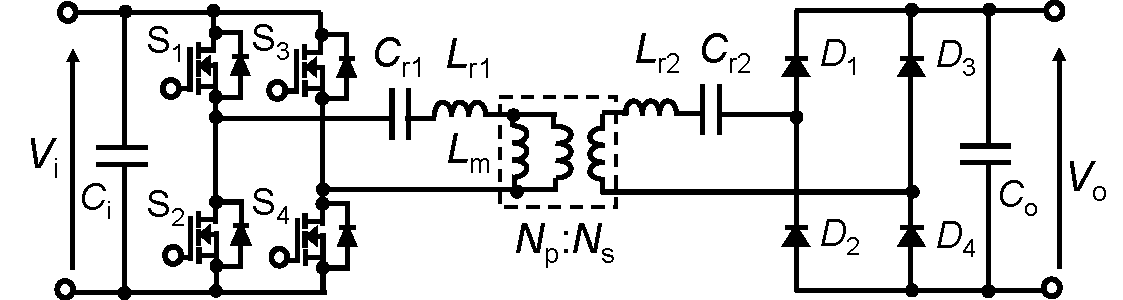
\includegraphics[width = \columnwidth]{figures_chapter2/setup.pdf}
    \caption{Circuit diagram used for simulation.} \label{fig:setup}
\end{figure}

Figure \ref{fig:100kWSim} shows the circuit simulation results at 100 kW for (a) 100\% load, (b) 50\% load, and (c) 20\% load. ZVS is achieved using the circuit parameters.

\begin{figure}[h!]
    \centering
    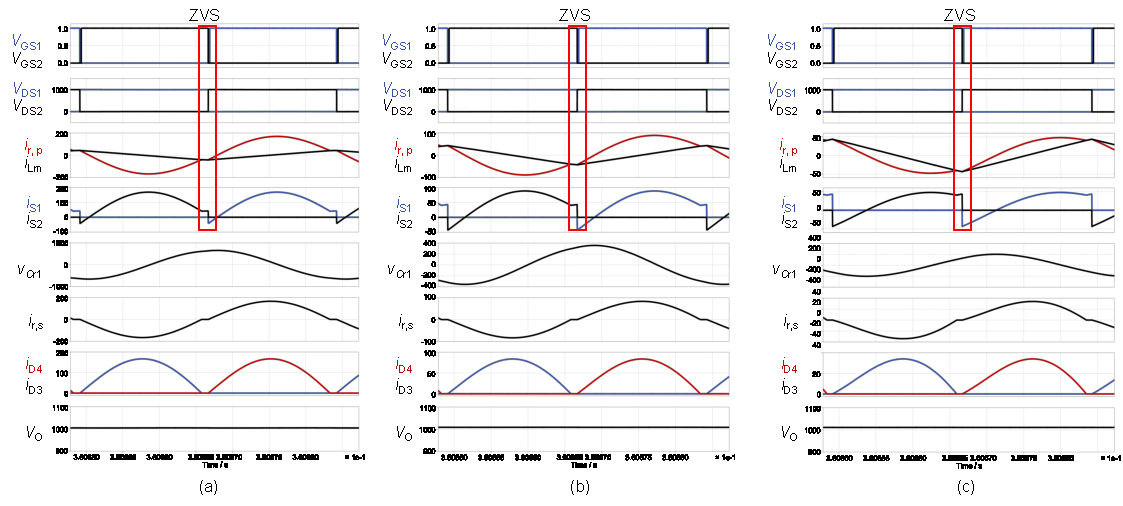
\includegraphics[width = \columnwidth]{figures_chapter2/100 kW compilation .pdf}
    \caption{100 kW circuit simulation results: (a) at 100\% load, (b) at 50 \% load, and (c) at 20\% load.} \label{fig:100kWSim}
\end{figure}

\pagebreak
Figure \ref{fig:1kWSim} shows the circuit simulation results at 1 kW for (a) 100\% load, (b) 50\% load, and (c) 20\% load. ZVS is achieved using the same resonant tank with the 100 kW circuit.

\begin{figure}[h!]
    \centering
    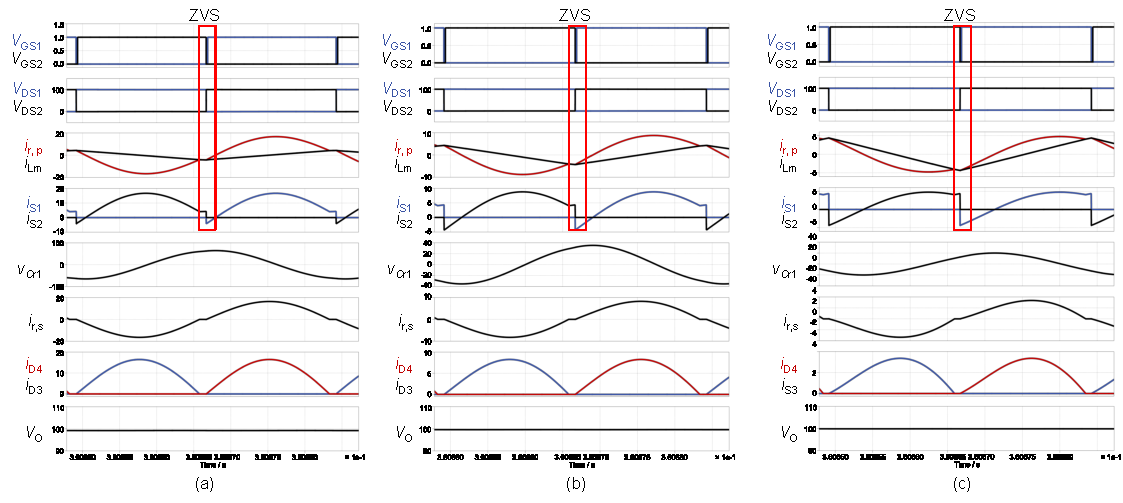
\includegraphics[width = \columnwidth]{figures_chapter2/1 kW compilation.pdf}
    \caption{1 kW circuit simulation results: (a) at 100\% load, (b) at 50 \% load, and (c) at 20\% load.} \label{fig:1kWSim}
\end{figure}

\pagebreak
For reference, the electrical circuit parameters used in the study are detailed in Table \ref{tab:power_electrical}, including the scalability analysis.

\begin{table}[h!]
\centering
\caption{Electrical Specifications for the Study}
\label{tab:power_electrical}
\begin{threeparttable}
\begin{tabular}{llccc}
\hline
\hline
\textbf{Parameter} & \textbf{Symbol} & \textbf{1 kW} & \textbf{10 kW} & \textbf{100 kW} \\
\hline
Input Voltage & $V_{\mathrm{in}}$ & 100 V & $316\text{ V } (\times\sqrt{10})$ & $1000\text{ V } (\times 10)$ \\
Output Voltage & $V_{\mathrm{o}}$ & 100 V & $316\text{ V } (\times\sqrt{10})$ & $1000\text{ V } (\times 10)$ \\
Output Current & $I_{\mathrm{o}}$ & 10 A & $31.6\text{ A } (\times\sqrt{10})$ & $100\text{ A } (\times 10)$ \\
Output Power & $P_{\mathrm{o}}$ & 1 kW & $10\text{ kW } (\times 10)$ & $100\text{ kW } (\times 100)$ \\
Switching Frequency\tnote{a}& $f_{\mathrm{sw}}$ & 15 -- 30 kHz & 15 -- 30 kHz & 15 -- 30 kHz \\
Resonant Frequency & $f_{\mathrm{r}}$ & 30.0 kHz & 30.0 kHz & 30.0 kHz \\
Dead Time & $t_{\mathrm{d}}$ & 360 ns & 360 ns & 360 ns \\
Resonant Capacitance & $C_{\mathrm{r1}}, C_{\mathrm{r2}}$ & $1.4~\upmu\text{F}$ & $1.4~\upmu\text{F}$ & $1.4~\upmu\text{F}$ \\
Resonant Inductance & $L_{\mathrm{r1}}, L_{\mathrm{r2}}$ & $20.1~\upmu\text{H}$ & $20.1~\upmu\text{H}$ & $20.1~\upmu\text{H}$ \\
Magnetizing Inductance & $L_{\mathrm{m}}$ & $200~\upmu\text{H}$ & $200~\upmu\text{H}$ & $200~\upmu\text{H}$ \\
\hline
\hline
\end{tabular}

\begin{tablenotes}
\small
\item[a] An $f_\mathrm{sw}$ of 28.5 kHz is chosen for this study.
\end{tablenotes}
\end{threeparttable}
\end{table}

\phantomsection
\chapter{Example Analytical Calculation}\label{app:model}
This appendix provides a detailed calculation example using the proposed analytical design methodology. The design space provided in Figure \ref{fig:trans_design} was generated computationally using Python, directly implementing the theoretical models established in Chapter 3. The calculations detailed here evaluate the specific flatwise-wound transformer design chosen for Tr2F, defined by $N_{\mathrm{p}} = 8$ turns and a wire width of $w_{\mathrm{wire}} = 0.30 \text{ mm}$.

\subsection*{Dimensioning and Volume Calculation}
To extract the physical footprint and total volume of the transformer, the wire height and core window dimensions must first be analytically defined. As established in Chapter 3, to satisfy a target current density ($J_{\mathrm{target}}$) under the nominal primary current ($I_{\mathrm{p,rms}}$), the required wire height ($h_{\mathrm{wire}}$) is governed by:
$$h_{\mathrm{wire}} = \frac{I_{\mathrm{p,rms}}}{J_{\mathrm{target}} \cdot w_{\mathrm{wire}}}$$
Substituting the design values ($J_{\mathrm{target}} = 5.0 \times 10^6 \text{ A/m}^2$, $I_{\mathrm{p,rms}} = 10.0 \text{ A}$):
$$h_{\mathrm{wire}} = \frac{10.0 \text{ A}}{(5.0 \times 10^6 \text{ A/m}^2) \cdot (0.3 \times 10^{-3} \text{ m})} = 6.67 \times 10^{-3} \text{ m} = 6.67 \text{ mm}$$

The core window height ($l_{\mathrm{win}}$) and width ($w_{\mathrm{win}}$) are geometrically constrained by the copper height, the total number of turns ($N_{\mathrm{p}}$), the inter-turn spacing ($d_{\mathrm{inter}}$), and the boundary clearances to the core ($d_{\mathrm{clear}}$):
$$l_{\mathrm{win}} = h_{\mathrm{wire}} + 2 d_{\mathrm{clear}}$$
$$w_{\mathrm{win}} = 2 N_{\mathrm{p}} w_{\mathrm{wire}} + (2 N_{\mathrm{p}} - 1) d_{\mathrm{inter}} + 2 d_{\mathrm{clear}}$$
Substituting $d_{\mathrm{clear}} = 1.0 \text{ mm}$ and $d_{\mathrm{inter}} = 0.1 \text{ mm}$:
$$l_{\mathrm{win}} = 6.67 \text{ mm} + 2 (1.0 \text{ mm}) = 8.67 \text{ mm}$$
$$w_{\mathrm{win}} = 2(8)(0.3 \text{ mm}) + (16 - 1)(0.1 \text{ mm}) + 2(1.0 \text{ mm}) = 8.30 \text{ mm}$$
This closely matches a square window profile ($8.67 \text{ mm} \approx 8.30 \text{ mm}$), balancing the core and copper cross-sections.

As detailed in Chapter 3, the core length ($l_{\mathrm{core}}$) is determined by equating the total magnetic circuit reluctance ($\mathcal{R}_{\mathrm{tot}}$) to the required magnetizing inductance ($L_{\mathrm{m}} = 200 \ \upmu\text{H}$):
$$\mathcal{R}_{\mathrm{tot}} = \mathcal{R}_{\mathrm{core}} + \mathcal{R}_{\mathrm{gap}} = \frac{N_{\mathrm{p}}^2}{L_{\mathrm{m}}}$$
A binary search algorithm was used to solve the 3D reluctance network across the center and outer legs taking into account the fringing effect correction described in \cite{muhlethaler2011novel}. The core length converges to $l_{\mathrm{core}} = 50.86 \text{ mm}$. 

The physical core dimensions ($l_{\mathrm{core}} \times w_{\mathrm{core}} \times h_{\mathrm{core}}$) are geometrically formulated by adding the outer core legs ($w_{\mathrm{out}} = 5.0 \text{ mm}$) and center leg width ($w_{\mathrm{cent}} = 10.0 \text{ mm}$):
$$w_{\mathrm{core}} = w_{\mathrm{cent}} + 2 w_{\mathrm{win}} + 2 w_{\mathrm{out}} = 10.0 \text{ mm} + 2 (8.3 \text{ mm}) + 2 (5.0 \text{ mm}) = 36.6 \text{ mm}$$
$$h_{\mathrm{core}} = l_{\mathrm{win}} + 2 w_{\mathrm{out}} = 8.67 \text{ mm} + 2 (5.0 \text{ mm}) = 18.67 \text{ mm}$$

The overall transformer bounding box dimensions ($l_{\mathrm{trans}} \times w_{\mathrm{trans}} \times h_{\mathrm{trans}}$) are formulated by incorporating the winding extensions outside the core window:
$$l_{\mathrm{trans}} = l_{\mathrm{core}} + 2 w_{\mathrm{win}} = 50.86 \text{ mm} + 2 (8.3 \text{ mm}) = 67.46 \text{ mm}$$
$$w_{\mathrm{trans}} = w_{\mathrm{core}} = 36.6 \text{ mm}$$
$$h_{\mathrm{trans}} = h_{\mathrm{core}} = 18.67 \text{ mm}$$
The final volumetric bounding box ($V_{\mathrm{box}}$) evaluates to:
$$V_{\mathrm{box}} = l_{\mathrm{trans}} \cdot w_{\mathrm{trans}} \cdot h_{\mathrm{trans}} = (67.46 \text{ mm}) \cdot (36.6 \text{ mm}) \cdot (18.67 \text{ mm}) = 46,116 \text{ mm}^3 \approx 46.1 \text{ cm}^3$$

Subtracting the non-ferrite window and air gap areas from the core footprint yields the true magnetic core volume ($V_{\mathrm{core}}$):
$$V_{\mathrm{core}} = l_{\mathrm{core}} \left[ (w_{\mathrm{core}} \cdot h_{\mathrm{core}}) - \left( 2(w_{\mathrm{win}} \cdot l_{\mathrm{win}}) + l_{\mathrm{g}}(2 w_{\mathrm{out}} + w_{\mathrm{cent}}) \right) \right]$$
$$ \begin{aligned}
    V_{\mathrm{core}} &= l_{\mathrm{core}} \left[ (w_{\mathrm{core}} \cdot h_{\mathrm{core}}) - \left( 2(w_{\mathrm{win}} \cdot l_{\mathrm{win}}) + l_{\mathrm{g}}(2 w_{\mathrm{out}} + w_{\mathrm{cent}}) \right) \right] \\
    &= 50.86 \left[ (36.6 \cdot 18.67) - \left( 2(8.3 \cdot 8.67) + 0.1(2(5.0) + 10.0) \right) \right] \text{ mm}^3 \\
    &= 27,332 \text{ mm}^3 = 2.73 \times 10^{-5} \text{ m}^3
\end{aligned} $$

\subsection*{Winding Geometry and Copper Loss}
With the physical dimensions locked, the unrolled length of the fully interleaved copper winding is analytically modeled as an arithmetic series. The inner perimeter of the first turn ($lt_1$) is derived from the center leg dimensions and internal clearances:
$$lt_1 = 2 \left[ (w_{\mathrm{cent}} + w_{\mathrm{wire}} + 2 d_{\mathrm{clear}}) + (l_{\mathrm{core}} + w_{\mathrm{wire}} + 2 d_{\mathrm{clear}}) \right]$$
$$lt_1 = 2 \left[ (10.0 + 0.3 + 2.0) \text{ mm} + (50.86 + 0.3 + 2.0) \text{ mm} \right] = 130.92 \text{ mm}$$
Because the flatwise turns stack radially outward, each subsequent turn increases in perimeter by a constant geometric difference $d$:
$$d = 8 (w_{\mathrm{wire}} + d_{\mathrm{inter}}) = 8 (0.3 \text{ mm} + 0.1 \text{ mm}) = 3.2 \text{ mm}$$
The total combined length of the primary and secondary copper ($S_{\mathrm{total}}$) is given by the series sum for $n = 2 N_{\mathrm{p}}$ total turns:
$$S_{\mathrm{total}} = N_{\mathrm{p}} \left[ 2 lt_1 + (2 N_{\mathrm{p}} - 1) d \right]$$
$$S_{\mathrm{total}} = 8 \left[ 2(130.92 \text{ mm}) + (16 - 1)(3.2 \text{ mm}) \right] = 2,478.7 \text{ mm} = 2.479 \text{ m}$$
Applying the fundamental resistance equation with the conductivity of copper ($\sigma = 5.96 \times 10^7 \text{ S/m}$), the base DC resistance ($R_{\mathrm{dc}}$) is:
$$ \begin{aligned}
    R_{\mathrm{dc}} &= \frac{S_{\mathrm{total}}}{\sigma \cdot h_{\mathrm{wire}} \cdot w_{\mathrm{wire}}} \\
    &= \frac{2.479 \text{ m}}{(5.96 \times 10^7 \text{ S/m}) \cdot (6.67 \times 10^{-3} \text{ m}) \cdot (0.3 \times 10^{-3} \text{ m})} \\
    &= 20.79 \times 10^{-3} \ \Omega = 20.79 \text{ m}\Omega
\end{aligned} $$
To account for high-frequency skin and proximity effects (Chapter 3), the skin depth ($\delta$) at $f_{\mathrm{s}} = 28.5 \text{ kHz}$ is calculated:
$$\delta = \frac{1}{\sqrt{\pi f_{\mathrm{s}} \mu_0 \sigma}} = \frac{1}{\sqrt{\pi (28,500 \text{ Hz}) (4\pi \times 10^{-7} \text{ H/m}) (5.96 \times 10^7 \text{ S/m})}} = 0.386 \text{ mm}$$
The penetration ratio ($\xi$) dictates the 1D Dowell's resistance factor ($F_{\mathrm{ac}}$). Moreover, for a fully-interleaved scenario, $m=1$ for all layers.
$$\xi = \frac{w_{\mathrm{wire}}}{\delta} = \frac{0.300 \text{ mm}}{0.386 \text{ mm}} = 0.777$$
$$F_{\mathrm{ac}} = \frac{\xi}{2} \left[ \frac{\sinh \xi + \sin \xi}{\cosh \xi - \cos \xi} + (2m^2-1)\frac{\sinh \xi - \sin \xi}{\cosh \xi + \cos \xi} \right] \approx 1.032$$
The total AC resistance ($R_{\mathrm{ac}}$) and resultant winding loss ($P_{\mathrm{wind}}$) are thus formulated as:
$$R_{\mathrm{ac}} = F_{\mathrm{ac}} R_{\mathrm{dc}} = (1.032) \cdot (20.79 \text{ m}\Omega) = 21.46 \text{ m}\Omega$$
$$P_{\mathrm{wind}} = I_{\mathrm{p,rms}}^2 R_{\mathrm{ac}} = (10.0 \text{ A})^2 \cdot (21.46 \times 10^{-3} \ \Omega) = 2.15 \text{ W}$$

\subsection*{Core Loss Computation}
As defined by Faraday's Law in Chapter 3, the core loss is driven by the flux density variation ($\Delta B$) over the switching half-period ($T_{\mathrm{s}}/2$). Using the cross-sectional core area $A_{\mathrm{calc}} = l_{\mathrm{core}} \cdot w_{\mathrm{cent}} = 508.6 \text{ mm}^2$:
$$\Delta B = \frac{V_{\mathrm{pri,pk}} (T_{\mathrm{s}}/2)}{N_{\mathrm{p}} A_{\mathrm{calc}}}$$
$$\Delta B = \frac{(100 \text{ V}) \cdot (17.54 \times 10^{-6} \text{ s})}{8 \cdot (508.6 \times 10^{-6} \text{ m}^2)} = 0.431 \text{ T}$$
Subtracting the $400 \text{ ns}$ deadtime yields an active excitation time of $17.14 \ \upmu\text{s}$, driving the time derivative of the magnetic flux:
$$\frac{dB}{dt} = \frac{\Delta B}{t_{\mathrm{active}}} = \frac{0.431 \text{ T}}{17.14 \times 10^{-6} \text{ s}} = 25,151 \text{ T/s}$$
The core loss is evaluated utilizing the Improved Generalized Steinmetz Equation (iGSE) with the manufacturer material parameters ($k = 0.0620, \alpha = 1.7066, \beta = 2.535$). The waveform coefficient ($k_i$) is defined analytically as:
$$k_i = \frac{k}{2\pi^{\alpha-1} \int_{0}^{2\pi} \vert \cos \theta \vert^{\alpha} 2^{\beta-\alpha} \, d\theta} \approx 2.331 \times 10^{-3}$$
Substituting the parameters yields the instantaneous volumetric loss density. Multiplied by the total derived core volume ($V_{\mathrm{core}} = 2.73 \times 10^{-5} \text{ m}^3$), the time-averaged core loss ($P_{\mathrm{core}}$) resolves to:
$$P_{\mathrm{core}} = \frac{V_{\mathrm{core}}}{T_{\mathrm{s}}} \int_{0}^{T_{\mathrm{s}}} k_i \left| \frac{dB}{dt} \right|^{\alpha} (\Delta B)^{\beta-\alpha} \, dt$$
$$P_{\mathrm{core}} = \frac{2.73 \times 10^{-5}}{35.09 \times 10^{-6}} \int_{0}^{35.09 \times 10^{-6}} (2.331 \times 10^{-3}) (25,151)^{1.7066} (0.431)^{0.8284} \, dt = 1.03 \text{ W}$$
Summing the analytically derived copper and core losses yields the total simulated power dissipation for the selected configuration:
$$P_{\mathrm{total}} = P_{\mathrm{wind}} + P_{\mathrm{core}} \approx 2.15 \text{ W} + 1.03 \text{ W} = 3.17 \text{ W}$$

\phantomsection
\chapter{Simulation Settings}\label{app:ansys}
This section details the simulation setup for the 3D Finite Element Analysis (FEA) environment Ansys.

\section*{Simulation Apparatus}
The parametric and finite element analyses were executed on a high-performance engineering workstation optimized for heavy electromagnetic and thermal simulation workloads. The essential hardware specifications of the workstation are summarized in Table \ref{tab:workstation}. The software utilized for all evaluations was Ansys 2023 R1.

\begin{table}[h!]
    \centering
    \caption{Workstation Hardware Specifications}
    \begin{tabular}{ll}
        \hline
        \textbf{Component} & \textbf{Specification} \\
        \hline \hline
        System Model & Dell Precision 5860 Tower \\
        Operating System & Windows 11 Pro for Workstations \\
        Processor & Intel Xeon w7-2475X (20 Cores, 40 Threads) \\
        Physical Memory (RAM) & 256 GB \\
        System Architecture & 64-bit (x64-based PC) \\
        \hline
    \end{tabular}
    \label{tab:workstation}
\end{table}

Ansys Electronics was specifically used. The Ansys Maxwell Environment was utilized for the Electromagnetic Simulations (Eddy Current) and Electrostatic SImulations (Electrostatic)

\section*{Material Parameters}
Before going in detail with the simulation environment setup, materials were setup first to ensure that the physical phenomena can be reproduced. It is important to note that the simulation is not aimed as a 1:1 correspondence with the actual model, as there will be many differences when devices are evaluated in real life. 

Particularly, the materials referred to the parts of the transformer described in Figure \ref{fig:flatwise_3D_trans} and \ref{fig:edgewise_2D_trans} pertaining to the EE core, windings, TIM between core and windings, and additional aluminum at the dead space were modeled in the materials modeler. 

It is important to note that because thermal simulations were performed, the thermal properties of the materials, specifically the \textbf{specific heat} and \textbf{thermal conductivity} were set appropriately according to data sheets or material property databases. The properties assigned to copper, the LP10A core, the Thermal Interface Material (TIM), air, and aluminum are consolidated in Table \ref{tab:material_properties}.

\begin{table}[h!]
    \centering
    \caption{Material Properties Assigned in Ansys FEA Simulations}
    \resizebox{\textwidth}{!}{
    \begin{tabular}{lccccc}
        \hline
        \textbf{Property (Unit)} & \textbf{Copper} & \textbf{Ferrite} & \textbf{TIM} & \textbf{Air} & \textbf{Aluminum} \\
        \hline \hline
        Relative Permittivity & 1 & 12 & 9 & 1.0006 & 1 \\
        Relative Permeability & 0.999991 & 3400 & 1 & 1.0000004 & 1.000021 \\
        Bulk Conductivity (S/m) & $5.8 \times 10^7$ & 0.25 & 0 & 0 & $3.8 \times 10^7$ \\
        Thermal Conductivity (W/m$\cdot$C) & 400 & 4 & 10 & 0.0261 & 237.5 \\
        Mass Density (kg/m$^3$) & 8933 & 4800 & 3700 & 1.1614 & 2689 \\
        Specific Heat (J/kg$\cdot$C) & 385 & 750 & 712 & 1005 & 951 \\
        Young's Modulus (N/m$^2$) & $1.2 \times 10^{11}$ & $1.19 \times 10^{11}$ & $1.35 \times 10^{11}$ & - & $6.9 \times 10^{10}$ \\
        Poisson's Ratio & 0.38 & 0 & 0.25 & - & 0.31 \\
        Thermal Expansion Coefficient (1/C) & $1.77 \times 10^{-5}$ & $1.0 \times 10^{-6}$ & $2.54 \times 10^{-6}$ & 0.00333 & $2.33 \times 10^{-5}$ \\
        Core Loss Model & - & Power Ferrite & - & - & - \\
        Steinmetz Coefficient $C_m$ ($k$) & - & 0.0620 & - & - & - \\
        Steinmetz Coefficient $X$ ($\alpha$) & - & 1.7066 & - & - & - \\
        Steinmetz Coefficient $Y$ ($\beta$) & - & 2.5355 & - & - & - \\
        Thermal Diffusivity (m$^2$/s) & - & - & - & $2.88 \times 10^{-5}$ & - \\
        Molecular Mass (kg/mol) & - & - & - & 0.028966 & - \\
        Dynamic Viscosity (kg/m$\cdot$s) & - & - & - & $1.84 \times 10^{-5}$ & - \\
        \hline
    \end{tabular}}
    \label{tab:material_properties}
\end{table}

A few additional notes are given on the material property assignments:
\begin{itemize}
    \item For the copper and aluminum, the default indicated by Ansys is used.
    \item For the air utilized in the region for natural convection in the thermal simulation, the default indicated by Ansys was used.
    \item For the TIM, the material by Laird Tflex SF10 was utilized. The applicable parameters from the datasheet were input into the software. 
    \item For the magnetic core, the core-loss density-magnetic flux density $P_{\mathrm{cv}}-B$ curve was input into the software as a power ferrite, after which the modeler gave the steinmetz parameters. The material used was MBT1 by JFE Corporation.  Although it was not the exact LP10A Mn-Zn ferrite core used in the experimental prototype, the magnetic properties and core loss characteristics within the evaluated operating region are highly comparable and very close to each other. In fact, the steinmetz parameters of both materials lead to almost same loss given the operating conditions when computed theoretically and by simulation. As a final note, the core was set with constant initial permeability. This was because the transformer was gapped in all legs, making the changes negligible becasue the gap dominates the overall reluctance of the magnetic circuit. Gaps were added to prevent saturation in the core.
\end{itemize}  

\section*{Mesh Settings}
\subsection*{Electromagnetic Simulation: Ansys Maxwell 3D Eddy Current}
A 3D simulation was utilized for the electromagnetic simulation. The core and aluminum components were given a 5 mm maximum length on selection. The copper winding was given a finer 2 mm length on selection. Although a finer mesh and lower error percentage is preferred, this was what the workstation could handle before running out of memory across all the parametric simulation cases. Symmetry techniques could be explored in future work, or 2D simulation might also be worth exploring. However, the researchers preferred having both core and copper losses simulated together to allow for a close simulation of the real operating condition. Moreover, the windings were modeled as solid, discrete conductors to explicitly resolve the high-frequency eddy current distributions without exceeding hardware limits.

\subsection*{Electrostatic Simulation: Ansys Maxwell 2D Electrostatic}

A 2D simulation was performed to evaluate the maximum electric field strength $E$-field in kV/mm between the primary and secondary winding layers, and also between the windings, core and the TIM. Because the longitudinal geometry of the planar transformer window is highly uniform, a 2D cross-sectional analysis provides sufficient accuracy while drastically reducing computational overhead. More detailed meshing was performed through selecting all elements and setting the mesh to edge-cut inside selection with a length of less than 0.05 mm. 

\subsection*{Thermal Simulation: Ansys Icepak 3D Steady-state}
A 3D simulation was performed to evaluate the temperature distribution over the component. The global mesh was configured utilizing the Auto Mesh Setting. The resolution slider was positioned to the maximum "Fine" setting to yield a "Large" mesh count. Additionally, the Facet Level was set to its maximum value (slider fully to the right) to ensure accurate representation of the component geometries. For the higher power simulations, mesh regions were applied for the edgewise-wound transformer simulations that encompass the entire TIM and windings. From here, either auto-mesh was used, or were set manually such that there are at least three elements in all axes.

\section*{Simulation Setup Settings}

\subsection*{Ansys Maxwell 3D Eddy Current Setup}
The electromagnetic evaluation utilized an adaptive mesh setup to capture core and copper losses with the following criteria:
\begin{itemize}
    \item \textbf{Air Region:} The internal non-solid domains were assigned as a vacuum ($\mu_r = 1$), which is electromagnetically indistinguishable from air for the purpose of magnetic loss evaluation. Furthermore, the external bounding region was configured with 0\% padding to strictly conserve computational memory. Moreover, this was chosen as the the critical fringing flux is expected to be localized entirely within the internal core window.
    \item \textbf{Adaptive Passes:} A maximum of 20 passes was permitted, with a target percent error of 1\%. The solver required a minimum of 2 passes and at least 1 converged pass.
    \item \textbf{Refinement:} The mesh refinement was set to 30\% per pass.
    \item \textbf{Matrix Solution:} The matrix was configured to solve after the last pass.
\end{itemize}

\subsection*{Ansys Maxwell 2D Electrostatic Setup}
The electrostatic evaluation utilized an adaptive mesh setup to capture core and copper losses with the following criteria:
\begin{itemize}
    \item \textbf{Air Region:} The internal non-solid domains were assigned with air, which is the chosen insulation material and also the surrounding environment of the transforme. Furthermore, the external bounding region was configured with 50\% padding in the $+Z$, $-Z$, and $+X$ directions.
    \item \textbf{Adaptive Passes:} A maximum of 20 passes was permitted, with a target percent error of 0.5\%. The solver required a minimum of 10 passes and at least 1 converged pass.
    \item \textbf{Refinement:} The mesh refinement was set to 70\% per pass.
    \item \textbf{Matrix Solution:} The matrix was configured to solve after the last pass.
    \item \textbf{Boundary Conditions:} A balloon charge boundary condition was placed on the bounding walls of the region on the $+Z$, $-Z$, and $+X$ directions. Symmetry was placed on the $-X$ bounding wall.
\end{itemize}


\subsection*{Ansys Icepak 3D Steady State Setup}
The Ansys Icepak configuration managed the thermal domains using the following exact parameters and meshing strategies. The ambient temperature was set to $25^\circ$C.
\begin{itemize}
    \item \textbf{Air Region:} The computational domain was padded with a Percentage Offset of 1000 in the $+X$, $-X$, $+Y$, $-Y$, $+Z$, and $-Z$ directions. This is to ensure that natural convection plumes and fluid boundaries are fully captured without artificial truncation.
    \item \textbf{General Solver Settings:} The problem was set to solve for Temperature and Flow within a Laminar flow regime, including gravity. A maximum of 10000 iterations was specified.
    \item \textbf{Convergence Criteria:} The residual convergence limits were rigorously configured to 0.001 for Flow, 1e-07 for Energy, 0.001 for Turbulent Kinetic Energy, 0.001 for Turbulent Dissipation Rate, 0.001 for Specific Dissipation, 1e-06 for Discrete Ordinates, and 1e-07 for Joule Heating.
    \item \textbf{Initial Conditions:} The initial velocities were set to 0 m/s for $X$ and $Y$, and 0.000980665 m/s for $Z$, with the temperature initialized at the ambient temperature.
    \item \textbf{Radiation Model:} The Discrete Ordinates radiation model was employed, utilizing 2 Theta Divisions, 2 Phi Divisions, 2 Theta Pixels, and 2 Phi Pixels. Flow Iterations per Radiation Iteration were set to 10.
    \item \textbf{Boundary Conditions:} An ambient pressure and zero-velocity opening were set in the $+Y$ and $-Y$ directions to simulate an environment without any external disturbances except the cooling system.
\end{itemize}

Coupling between the Ansys Maxwell 3D Eddy Current solver and Ansys Icepak was established to map the volumetric power loss profile from the electromagnetic simulation directly into the thermal domain as the primary heat source through an EM Loss boundary condition. The corresponding parts were linked to each other. The TIM practically had no dielectric loss, and thus was excluded. The electromagnetic simulations were simulated as needed before being mapped into the thermal domain.
\end{document}
